\documentclass[12pt, a4paper]{report}

\usepackage{indentfirst}
\usepackage{fontspec}
\usepackage{polyglossia}
\usepackage[
backend = biber,
maxbibnames=50,
style=numeric,
sorting=nyt,
urldate=iso,
date=iso,
seconds=true
]{biblatex}
\DefineBibliographyExtras{english}{%
	\def\finalandcomma{\addcomma\space}%
	\def\finalandsemicolon{\addsemicolon\space}%
}
\usepackage{setspace}
\usepackage{geometry}
\usepackage{graphicx}
\usepackage{float}
\usepackage{amsmath}
\usepackage{xcolor}
\usepackage{mathtools}
\usepackage[warnings-off={mathtools-colon,mathtools-overbracket}]{unicode-math}

\usepackage{appendix}
\usepackage{caption}
\captionsetup[table]{name=Tabelul}
\usepackage{tabularray}
\usepackage{subcaption}
\usepackage[
colorlinks,
linkcolor={black},
menucolor={black},
citecolor={blue},
urlcolor={blue}
]{hyperref}


\usepackage{listings}
\usepackage{color}
\definecolor{codegreen}{rgb}{0,0.6,0}
\definecolor{codegray}{rgb}{0.5,0.5,0.5}
\definecolor{codepurple}{rgb}{0.58,0,0.82}
\definecolor{backcolour}{rgb}{0.95,0.95,0.92}
\definecolor{string}{rgb}{0.58,0.0,0.58}


\lstdefinelanguage{Python}{
	keywords={and, as, assert, async, await, break, class, continue, def, del, elif, else, except, False, finally, for, from, global, if, import, in, is, lambda, None, nonlocal, not, or, pass, raise, return, True, try, while, with, yield, pymupdf, io},
	keywordstyle=\color{blue}\bfseries,
	ndkeywords={append, get\_text, close, load\_page, get\_pixmap, open, tobytes, contains, color\_topusage, get\_images, get\_image\_info, transpose, pil\_save},
	ndkeywordstyle=\color{cyan}\bfseries,
	identifierstyle=\color{black},
	sensitive=true,
	comment=[l]{\#},
	morecomment=[s]{"""}{"""},
	commentstyle=\color{teal}\ttfamily,
	stringstyle=\color{teal}\ttfamily,
	morestring=[b]',
	morestring=[b]"
}

\lstset{
	backgroundcolor=\color{black!5},
	commentstyle=\color{green!40!black},
	keywordstyle=\color{blue!80!black}, 
	numberstyle=\tiny\color{gray!80!black},
	stringstyle=\color{string},
	basicstyle=\ttfamily\footnotesize,
	breakatwhitespace=false,
	breaklines=true,
	captionpos=b,
	keepspaces=true,
	numbers=left,
	numbersep=5pt,
	showspaces=false,
	showstringspaces=false,
	showtabs=false,
	tabsize=2,
	language=Python
}


\setdefaultlanguage{romanian}
\setotherlanguages{english}

\usepackage{csquotes}

\DeclareQuoteStyle{romanian}
  {\quotedblbase}
  {\textquotedblright}
  {\guillemotleft}
  {\guillemotright}
  
\DeclareFieldFormat{urldate}{%
	 (Data accesării: \ifnum\thefield{urlday}<10 0\fi\thefield{urlday}.\ifnum\thefield{urlmonth}<10 0\fi\thefield{urlmonth}.\thefield{urlyear})}

\addbibresource{bibliography.bib}

\graphicspath{{./images/}}

\newcommand{\bigO}[1]{\symcal{O}\left(#1\right)}
\DeclarePairedDelimiter\abs{\lvert}{\rvert}

\newenvironment{abstractpage}
  {\cleardoublepage\vspace*{\fill}\thispagestyle{empty}}
  {\vfill\cleardoublepage}
\renewenvironment{abstract}[1]
  {\bigskip\selectlanguage{#1}%
   \begin{center}\bfseries\abstractname\end{center}}
  {\par\bigskip}


\title{APLICAȚIE DE CONVERSIE A MANUALELOR DIN PDF ÎN HTML}
\author{Onuțu Radu-Constantin}

\makeatletter

\begin{document}

\cleardoublepage
\pagestyle{plain}
\begin{titlepage}


\newgeometry{left=2cm,right=2cm,bottom=1cm}

\begin{figure}[!htb]
    \centering
    \begin{minipage}{0.2\textwidth}
        
\includegraphics[width=\linewidth]{logo-ub.png}
    \end{minipage}
    \begin{minipage}{0.5\textwidth}
        \large
        \vspace{0.2cm}
        \begin{center}
            \textbf{UNIVERSITATEA DIN BUCUREȘTI}
        \end{center}
        \vspace{0.3cm}
        \begin{center}
            \textbf{
                FACULTATEA DE \\
                MATEMATICĂ ȘI INFORMATICĂ
            }
        \end{center}
    \end{minipage}
    \begin{minipage}{0.2\textwidth}
        
\includegraphics[width=\linewidth]{logo-fmi.png}
    \end{minipage}
\end{figure}

\begin{center}
\textbf{SPECIALIZAREA MATEMATICĂ-INFORMATICĂ}
\end{center}

\vspace{1cm}

\begin{center}
\Large \textbf{Lucrare de licență}
\end{center}

\begin{center}
\huge \textbf{\MakeUppercase{\@title}}
\end{center}

\vspace{3cm}

\begin{center}
\large \textbf{Absolvent \\ \@author}
\end{center}

\vspace{0.25cm}

\begin{center}
\large \textbf{Coordonator științific \\ Prof. dr. Andrei Păun}
\end{center}

\vspace{2cm}

\begin{center}
\Large \textbf{București, iunie 2024}
\end{center}
\end{titlepage}
\restoregeometry
\newgeometry{
    margin=2.5cm
}


\addtocounter{page}{1}

\begin{abstractpage}
\begin{abstract}{romanian}
	
Educația este esențială într-o societate și este important ca manualele școlare să aibă o calitate cât mai ridicată. În fiecare an, Ministerul Educației organizează licitații cu scopul de a achiziționa manuale cu un raport calitate-preț optim. Pe lângă variantele tipărite, Ministerul propune și crearea variantelor digitale ale acestor manuale.

Două dintre avantajele manualelor digitale sunt posibilitatea de a fi accesate de oriunde, precum și reducerea volumului de cărți pe care elevii îl transportă zilnic la școală.

Editura Intuitext are experiență de mai mulți ani în crearea manualelor și caută să își optimizeze procesul de creare în fiecare an. Până acum, transformarea manualelor în format digital era un proces care necesita foarte mult timp, atenție și resurse umane. Fiind un proces manual, riscul de erori era ridicat.

În această lucrare este descrisă  o aplicație de automatizare prin care se optimizează conversia manualelor tipărite în format digital, având ca obiectiv obținerea unui procent de similaritate cât mai ridicat. Acest proces eficient contribuie indirect la creșterea profitabilității editurii Intuitext.

\end{abstract}
\end{abstractpage}







\begin{abstractpage}
\begin{abstract}{english}
	
Education is essential in a society, and it is important for textbooks to be of the highest quality. Every year, the Ministry of Education organizes tenders to purchase textbooks with an optimal quality-price ratio. In addition to printed versions, the Ministry also advocates for the creation of digital textbooks.

Two of the advantages of digital textbooks are their accessibility from anywhere, as well as the reduction in the volume of books that students carry daily to school.

Intuitext publishing house, with many years of experience in creating textbooks, seeks to optimize its creation process every year. Until now, converting textbooks into digital format has been a time-consuming process requiring significant attention and human resources. This manual process carried a high risk of errors.

This paper describes an automation software that optimizes the conversion of printed textbooks into digital format, ensuring a high similarity percentage. This efficient process indirectly contributes to the profitability of the Intuitext publishing house.

\end{abstract}
\end{abstractpage}

\tableofcontents

\cleardoublepage

\cleardoublepage
\phantomsection
\addcontentsline{toc}{chapter}{\listfigurename}
\listoffigures

\cleardoublepage
\phantomsection
\addcontentsline{toc}{chapter}{\listtablename}
\listoftables 


\chapter{Introducere}
\section{Context}

Ministerul Educației Naționale (MEN) își propune cumpărarea manualelor școlare la un preț cât mai avantajos și cu o calitate cât mai bună \cite{minister}. Astfel, prin intermediul Centrului Național de Evaluare și Examinare (CNEE), Ministerul organizează anual licitații deschise pentru achiziționarea acestora. Pentru fiecare tip de manual (de exemplu, un manual de matematică pentru clasa a VI-a), Ministerul încheie contracte cu editurile pe o perioadă de 4 ani, după care sunt organizate noi licitații.

Evaluarea manualelor se bazează pe criterii tehnice, iar pentru ca un manual să fie declarat câștigător, acesta trebuie să obțină un punctaj de cel puțin 95 de puncte din 100. La un singur manual, pot câștiga mai multe edituri dacă această condiție este îndeplinită. Manualele trebuie să respecte un caiet de sarcini stabilit de MEN și CNEE. Astfel, câteva cerințe generale privind manualele digitale sunt: 
\begin{itemize}
	\item Accesarea manualului digital se face printr-un fișier de tip "index.html".
	\item Folderul director să nu depășească 600 MB.
	\item Paginile HTML să fie responsive (la o rezoluție de 1024x768 pixeli să nu apară bare de scroll orizontale).
	\item Manualul să poată fi utilizat pe fiecare browser din această listă: Google Chrome 31+, Mozilla Firefox 25+, Internet Explorer 10+, Safari 7+.
	\item Varianta digitală să cuprindă integral conținutul manualului din varianta tipărită.
\end{itemize}

Procesul de creare a unui manual tipărit și a unui manual digital se desfășoară conform următoarei diagrame:
\begin{figure}[H]
	\centering
	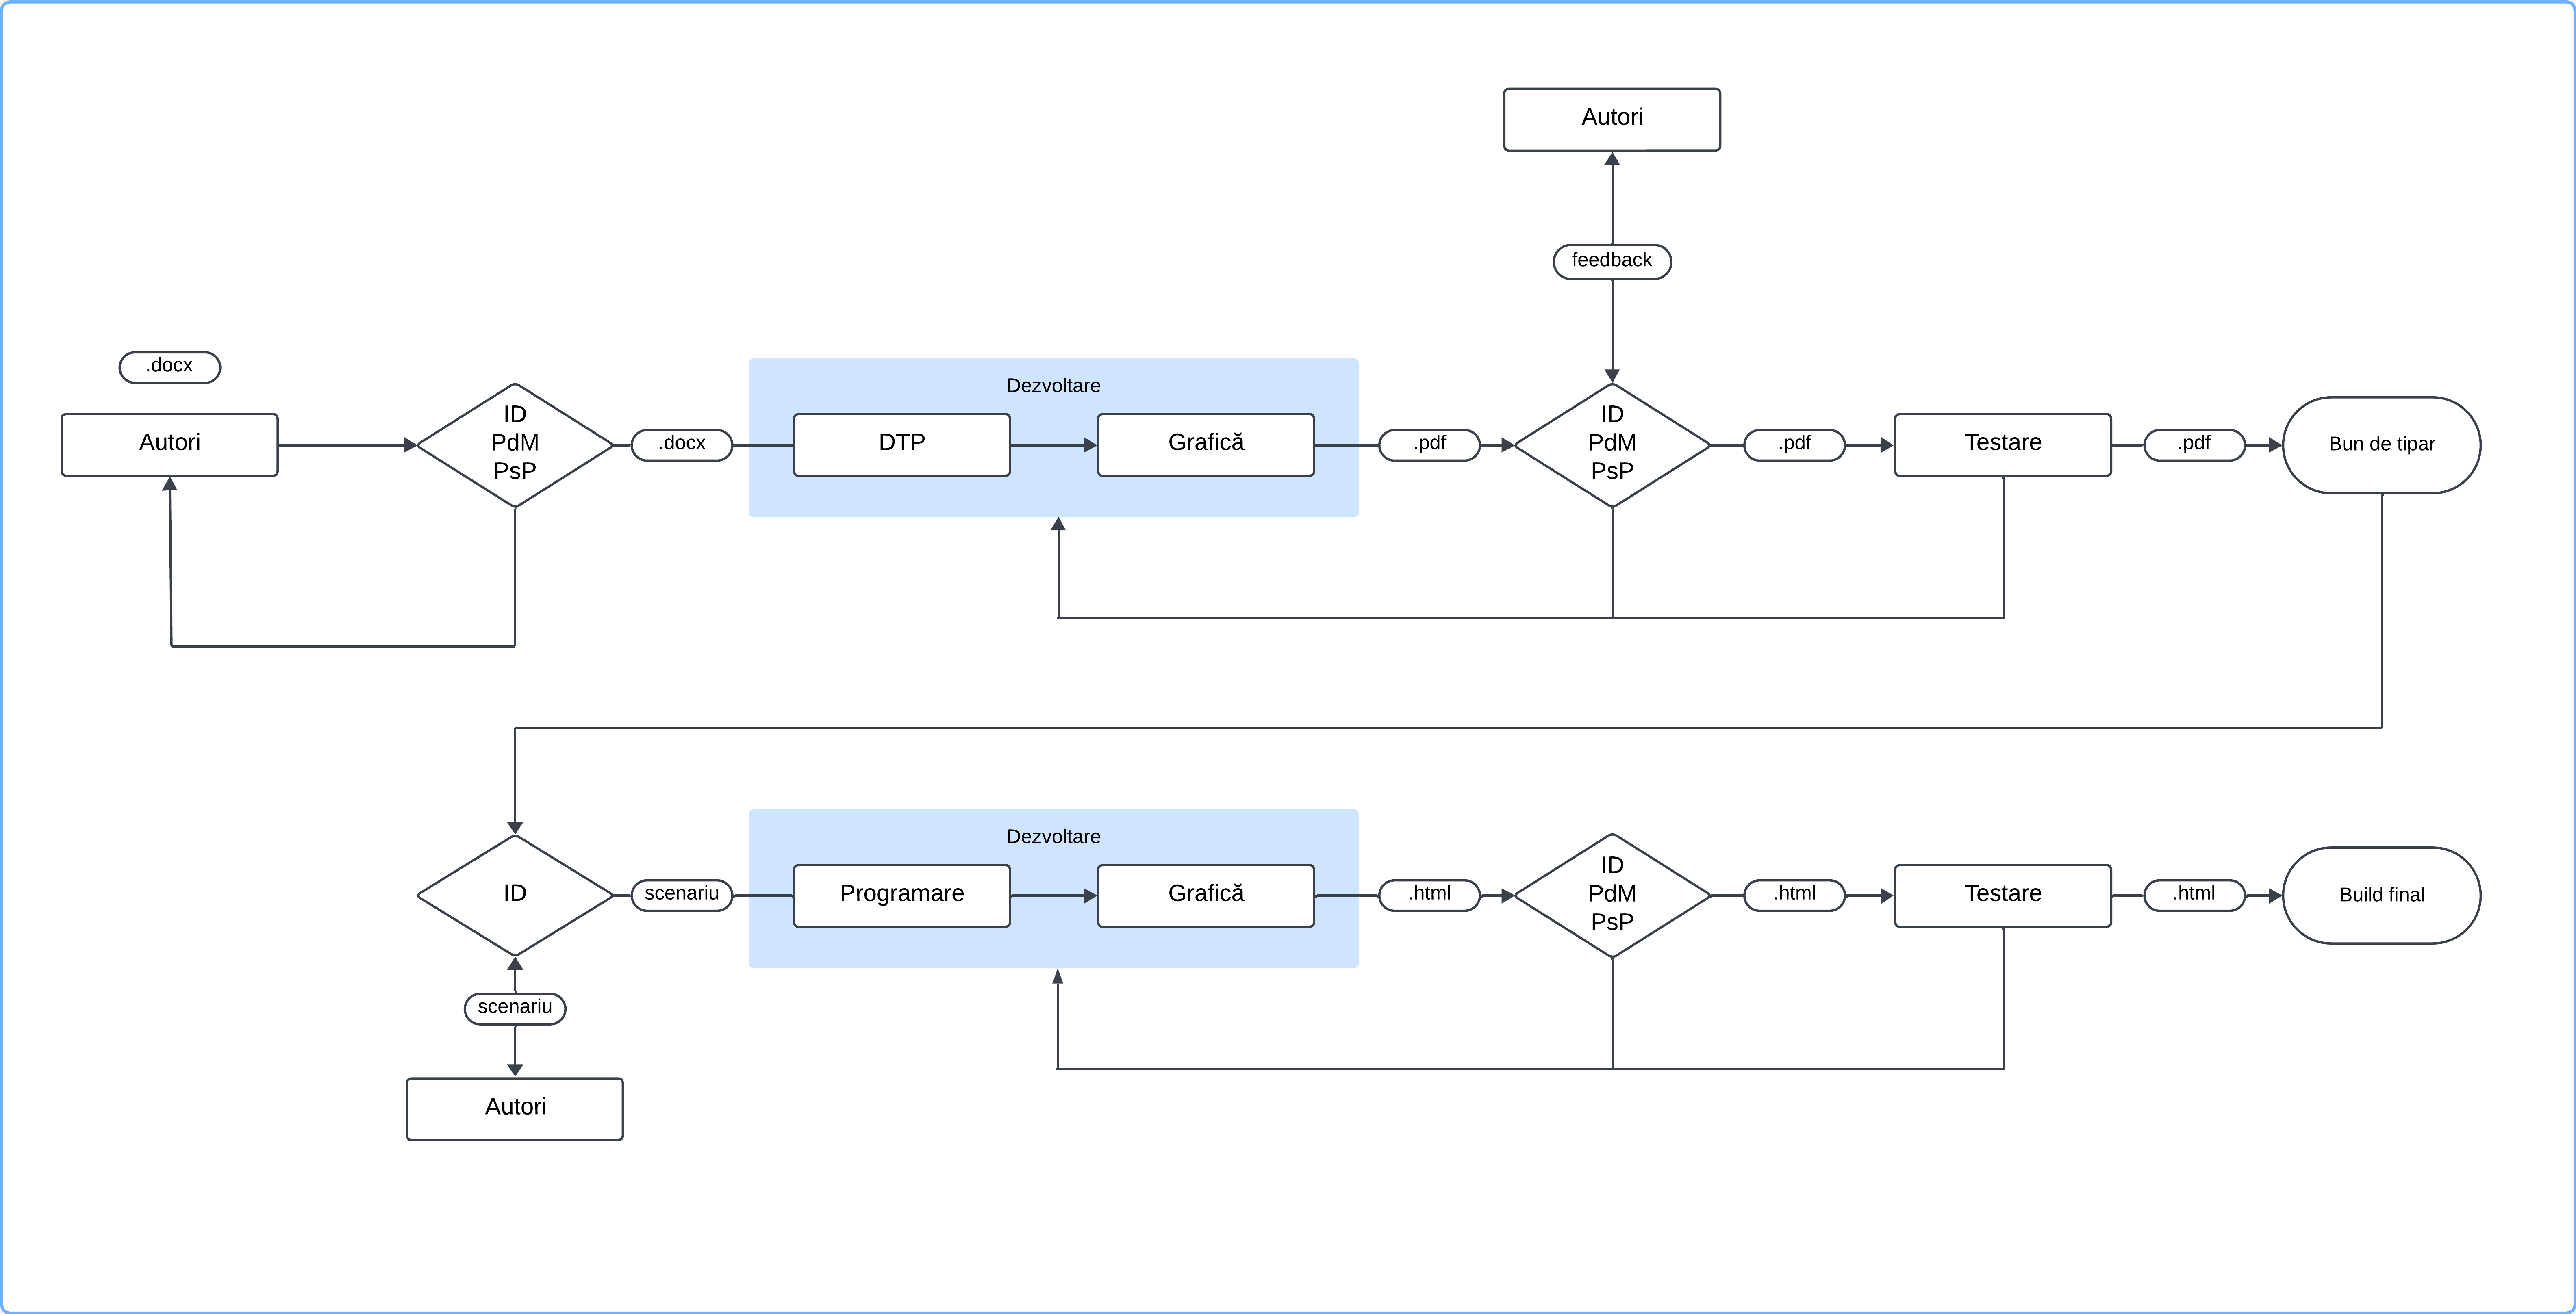
\includegraphics[scale=.3]{Figura1_1}
	\caption{Procesul de creare a manualelor tipărite și digitale}
	\label{fig:Figura1_1}
\end{figure}

\noindent
Legendă:
\begin{itemize}
	\item \textbf{ID} - Instructional Designer; persoana care pune în pagină conținutul și care creează un design pentru manual.
	\item \textbf{PdM} - Product Manager; persoana care supervizează tot procesul de creare.
	\item \textbf{PsP} - Psihopedagogic; persoana care propune modificări pentru conținut.
	\item \textbf{DTP} - Desktop Publishing; procesul prin care un manual este creat pentru a fi tipărit.
	\item \textbf{Grafică} - pasul în care se creează imaginile.
	\item \textbf{Programare} - procesul de a scrie cod HTML pentru conținutul dat de ID.
\end{itemize}

Procedura de creare pornește de la autori. Aceștia realizează un manuscris în format DOCX cu informațiile care vor apărea în manual. Ulterior, ID-ul, PdM-ul și PsP-ul verifică documentul și decid dacă sunt modificări de făcut. În momentul în care documentul este validat, procesul se împarte în două ramuri; o ramură pentru partea de tipar și alta pentru partea digitală.

Pentru dezvoltarea manualului de tipar, ID-ul structurează conținutul și toate detaliile care țin de punerea în pagină, iar după aceea echipa de grafică creează imagini. Tehnologiile folosite în acest proces sunt Adobe InDesign și Adobe Illustrator.

Adobe InDesign este o aplicație complexă de creare și structurare a documentelor, care poate să genereze documente cu rolul de a fi tipărite \cite{adobe2007adobe}. În cadrul realizării manualelor în format PDF, această aplicație este folosită pentru a pune în pagină informațiile date de autori într-un mod structurat și uniform.

Adobe Illustrator este un program de design grafic folosit pentru crearea de ilustrații, logo-uri sau chiar diagrame \cite{tupper2021}. În cazul manualelor, programul este folosit pentru a crea diferite imagini asociate cu textul, care îmbunătățesc aspectul vizual.

După acești pași, va rezulta o variantă inițială a manualului, exportată din Adobe InDesign în format PDF. Din acest punct se fac  verificări, atât pe partea de conținut dată de autori, cât și pe partea de redactare realizată de ID. Dacă nu există greșeli, se exportă manualul în versiunea lui finală. Dacă apar greșeli, se reiau pașii anteriori.

În diagrama de mai sus, la a doua parte de dezvoltare se sare peste pasul de grafică deoarece imaginile sunt obținute de la prima parte de dezvoltare, cea a manualului tipărit.

Manualul digital este creat într-un mod direct. După ce manualul este disponibil în format PDF, textul din acesta este extras și plasat într-un fișier HTML, împreună cu clasele și stilurile necesare. Deși este un proces simplu, acesta poate să dureze până la trei săptămâni pentru un manual de 200 de pagini. 


\section{Motivație}

În calitate de angajat al editurii Intuitext, am lucrat pe partea de conversie a manualelor în format digital și am observat cât de repetitiv este procesul și de cât de multă atenție este nevoie la detalii. Fiind un volum mare de manuale, riscul de a face greșeli era ridicat. În procesul de creare a manualului digital, orice greșeală reparată necesita retrimiterea manualului către echipa de testare până când toate erorile erau corectate. Acest lucru prelungea timpul în care un manual digital era finalizat.

Din dorința de a optimiza acest proces meticulos, am venit cu propunerea de a crea o aplicație care să automatizeze conversia.

Aplicația se folosește de datele pe care le extrage din manualul în format PDF: mărimea textului, fontul, culoarea textului, culoarea de fundal. Pe baza acestor date, aplicația recunoaște ce stiluri trebuie aplicate asupra textului și le scrie într-un fișier HTML. Fiecărei pagini din manualul tipărit i se asociază câte o pagină HTML.


\section{Scopul lucrării}

Scopul aplicației descrise în această lucrare este de a reduce timpul pe care angajații îl consumă pentru a converti manuale din format PDF în format HMTL. Beneficiul principal al acestei aplicații este creșterea profitabilității companiei într-un mod indirect. Timpul petrecut de angajați pentru transformarea manualelor va fi redirecționat către alte proiecte.

Un alt avantaj al aplicației este reducerea intervenției umane în procesul de transformare, ceea ce diminuează riscul apariției greșelilor. Acest lucru conduce la economisirea unui timp suplimentar deoarece nu trebuie să se reia pasul de testare de foarte multe ori.

În caietul de sarcini dat de MEN și CNEE este menționat faptul că tot conținutul din varianta de tipar a unui manual trebuie să apară și în varianta digitală, dar nu este nicio regulă care să precizeze că manualele trebuie să păstreze aceeași formatare.

Acest lucru ușurează procesul de automatizare deoarece permite schimbarea structurii unei pagini cât timp se păstrează ordinea logică a elementelor. De exemplu, unele pagini sunt împărțite în două coloane cu exerciții pe stânga și pe dreapta; nu este necesar să fie păstrată aceeași formatare atât timp cât se păstrează ordinea conținutului.


\section{Domenii abordate}

Domeniile abordate pentru realizarea aplicației sunt:
\begin{itemize}
	\item \textbf{Software development} - aplicația a fost dezvoltată folosind tehnici de bază, într-un mod simplu și eficient.
	\item \textbf{Automatizarea} - procesul de conversie a manualelor din format PDF în format HTML.
	\item \textbf{Natural Language Processing} - subdomeniu al inteligenței aritificiale, utilizat pentru a recunoaște structuri de text pe baza unor criterii.
\end{itemize}

 
\section{Obiective}

Pe parcursul dezvoltării aplicației, s-a ținut cont de următoarele aspecte:
\begin{itemize}
	\item \textbf{Similaritatea}: manualul digital generat să conțină într-o proporție cât mai mare elementele care sunt și în varianta tipărită.
	\item \textbf{Simplitatea}: structura codului HTML să fie organizată într-un mod cât mai ușor de modificat de alte persoane.
	\item \textbf{Viteza}: timpul de procesare să fie cât mai scurt.
	\item \textbf{Adaptabilitatea}: aplicația de automatizare să poată fi folosită pentru orice tip de manual, indiferent de materie sau de clasă.
\end{itemize}


\section{Structura lucrării}

Lucrarea este structurată în următoarele capitole:
\begin{itemize}
 	\item \textbf{Introducere}: prezintă scopul aplicației și aspectele care au fost luate în considerare la dezvoltarea acesteia.
 	\item \textbf{Soluții similare}: descrie soluțiile existente pe piață, le analizează și indică limitele sau inconvenientele lor.
 	\item \textbf{Tehnologii folosite}: detaliază tehnologiile alese pentru această aplicație și motivele pentru care au fost selectate.
 	\item \textbf{Soluție propusă}: este împărțită în patru subcapitole mai mici. Urmează cursul unui proces de automatizare: citirea, curățarea, gruparea și scrierea. 
	\item \textbf{Concluzii}: prezintă rezultatele aplicației și aspectele care pot fi îmbunătățite pe viitor. 
\end{itemize}

În subcapitolul de citire este descrisă metoda de extragere a informațiilor din documentul PDF, inclusiv extragerea imaginilor și procesul de obținere a culorii de fundal a textului.

În subcapitolul de curățare sunt identificate și șterse segmentele de text care nu vor apărea în varianta digitală.

În subcapitolul al treilea se prezintă metoda de grupare a textului în funcție de paragraful din care face parte.

În ultimul subcapitol se realizează procesul de scriere în fișierul HMTL și sunt identificate segmentele de text care nu au fost recunoscute de program și care vor fi introduse manual.

\chapter{Soluții similare}
\section{Prezentare generală a formatului PDF}

Portable Document Format (PDF) este un tip de fișier dezvoltat de Adobe în anul 1992. La baza acestui fișier stă PostScript, un limbaj de descriere a paginilor. Fiecare document PDF conține o descriere completă a structurii, a textului, a imaginilor și alte informații.

Formatul PDF oferă multe detalii despre fișier, ceea ce permite cu ușurință creearea de aplicații de convertire a documentelor în format HTML. Acestea există de mai bine de 26 ani \cite{kieninger1998paper} și folosesc diferite metode pentru a realiza transformarea. În capitolele următoare sunt analizate câteva dintre soluțiile de convertire existente, dar și motivele pentru care nu sunt adecvate în raport cu cerințele date de Minister.

Criteriile principale căutate sunt: posibilitatea de a selecta textul din fișierul HTML la afișare, paginile să fie responsive, codul să fie scris într-un mod ușor de editat.


\section{Conversia în imagini}

Metoda de conversie în imagini constă în transformarea paginilor din manuale PDF în imagini, urmată de inserarea acestora în fișiere HTML. Această metodă este simplă și rapidă din punct de vedere al implementării, dar nu îndeplinește cerințele cerute, deoarece textul nu poate fi selectat.

Pe lângă acest dezavantaj, mai apare și problema dimensiunii imaginilor. Transformarea paginilor în imagini are ca rezultat un folder director de dimensiuni mari care ar putea să depășească limita maximă admisă din caietul de sarcini.
\begin{figure}[H]
	\centering
	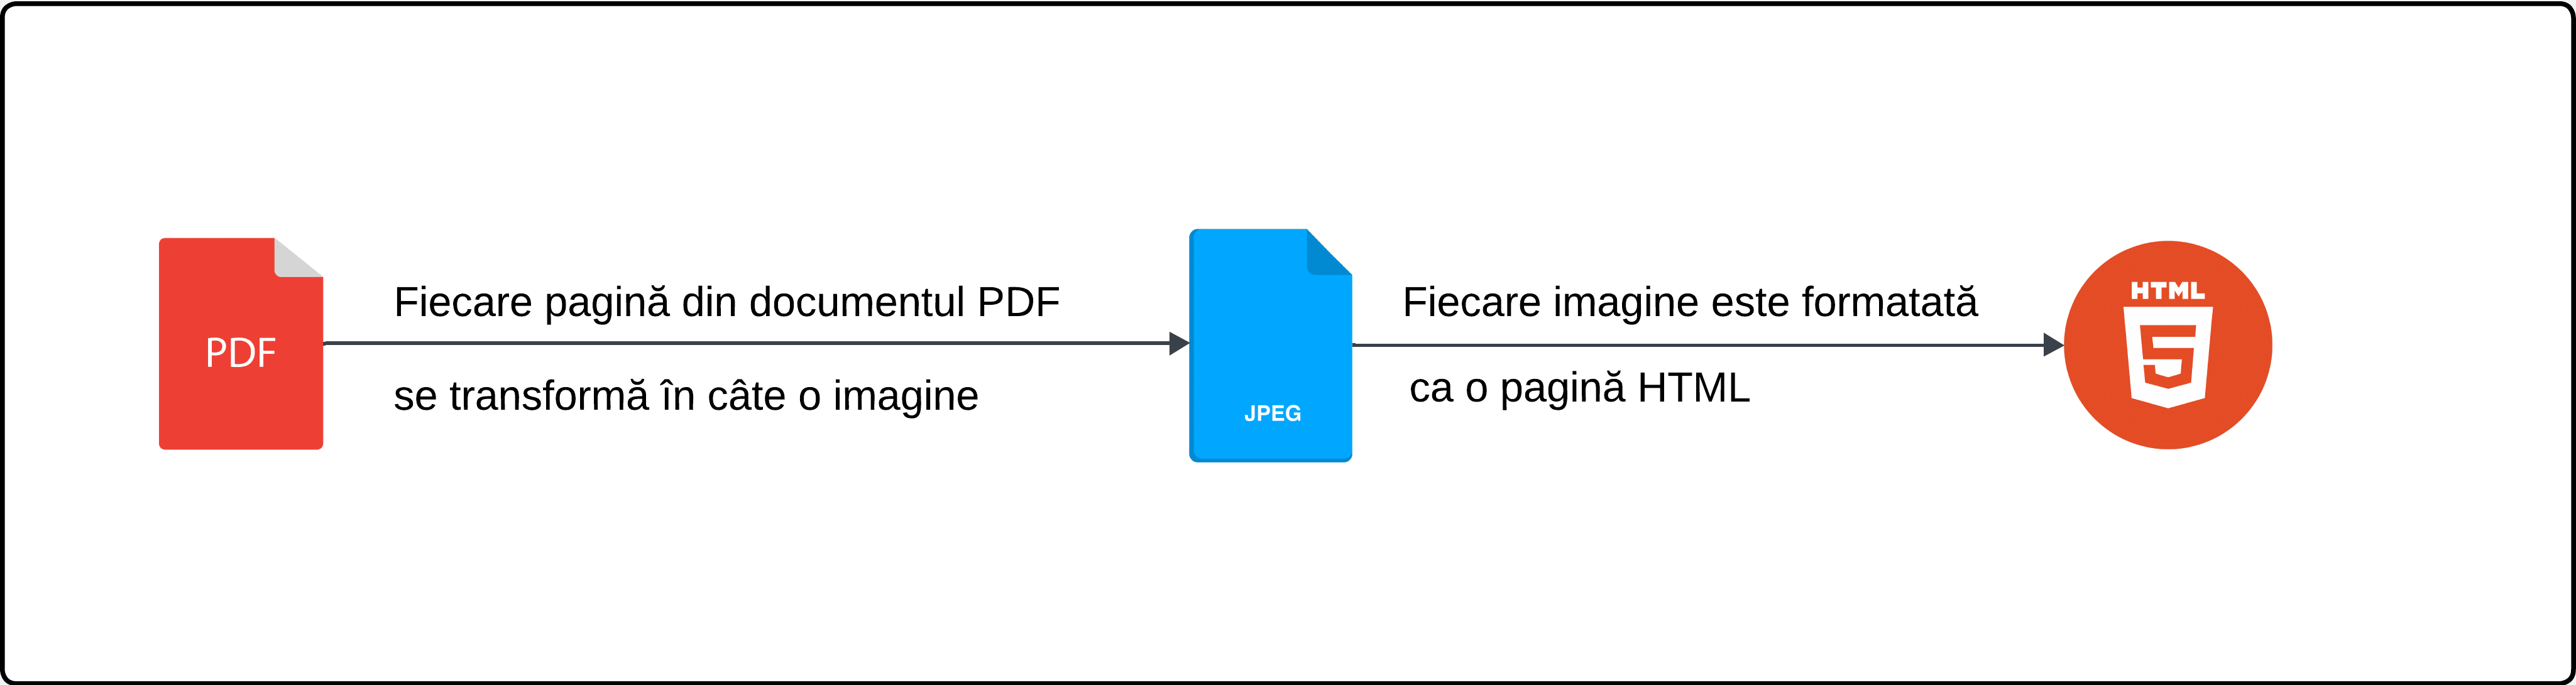
\includegraphics[scale=.4]{Figura2_1}
	\caption{Procesul de transformare a documentului PDF prin convertirea în imagini}
	\label{fig:Figura2_1}
\end{figure}


\section{Soluția de conversie de la Adobe Acrobat Pro}

Adobe Acrobat \cite{padova2008adobe} este o aplicație dezvoltată de Adobe, utilizată în toată lumea pentru crearea, manipularea, afișarea și gestionarea documentelor PDF.

Una dintre funcționalitățile sale este conversia documentelor PDF în format HTML, disponibilă numai în varianta cu plată a software-ului (Adobe Acrobat Pro). Acest lucru reprezintă un inconvenient pentru cazul de față.
\vspace{1em}

\noindent
Dezavantaje:
\begin{itemize}
	\item formatare greșită a textului;
	\item accesibil doar pentru varianta plătită.
\end{itemize}



\section{XHTML 1.0 Transitional}
\subsection{Soluția Xodo}

Extensible HyperText Markup Language (XHTML) \cite{musciano2006html} este un limbaj folosit pentru crearea și afișarea paginilor web. Acesta este foarte similar cu HTML (HyperText Markup Language), dar include câteva restricții suplimentare. XHTML este o versiune de HTML bazată pe formatul XML, care nu permite, de exemplu, lăsarea tagurilor deschise.

Xodo este un instrument care transformă documente PDF în format XHTML. Acesta permite o singură conversie gratuită pe zi și nu oferă rezultate bune. Structura documentului se desparte greșit și nu respectă culoarea de fundal.
\begin{figure}[H]
	\centering
	\begin{subfigure}{.5\textwidth}
		\centering
		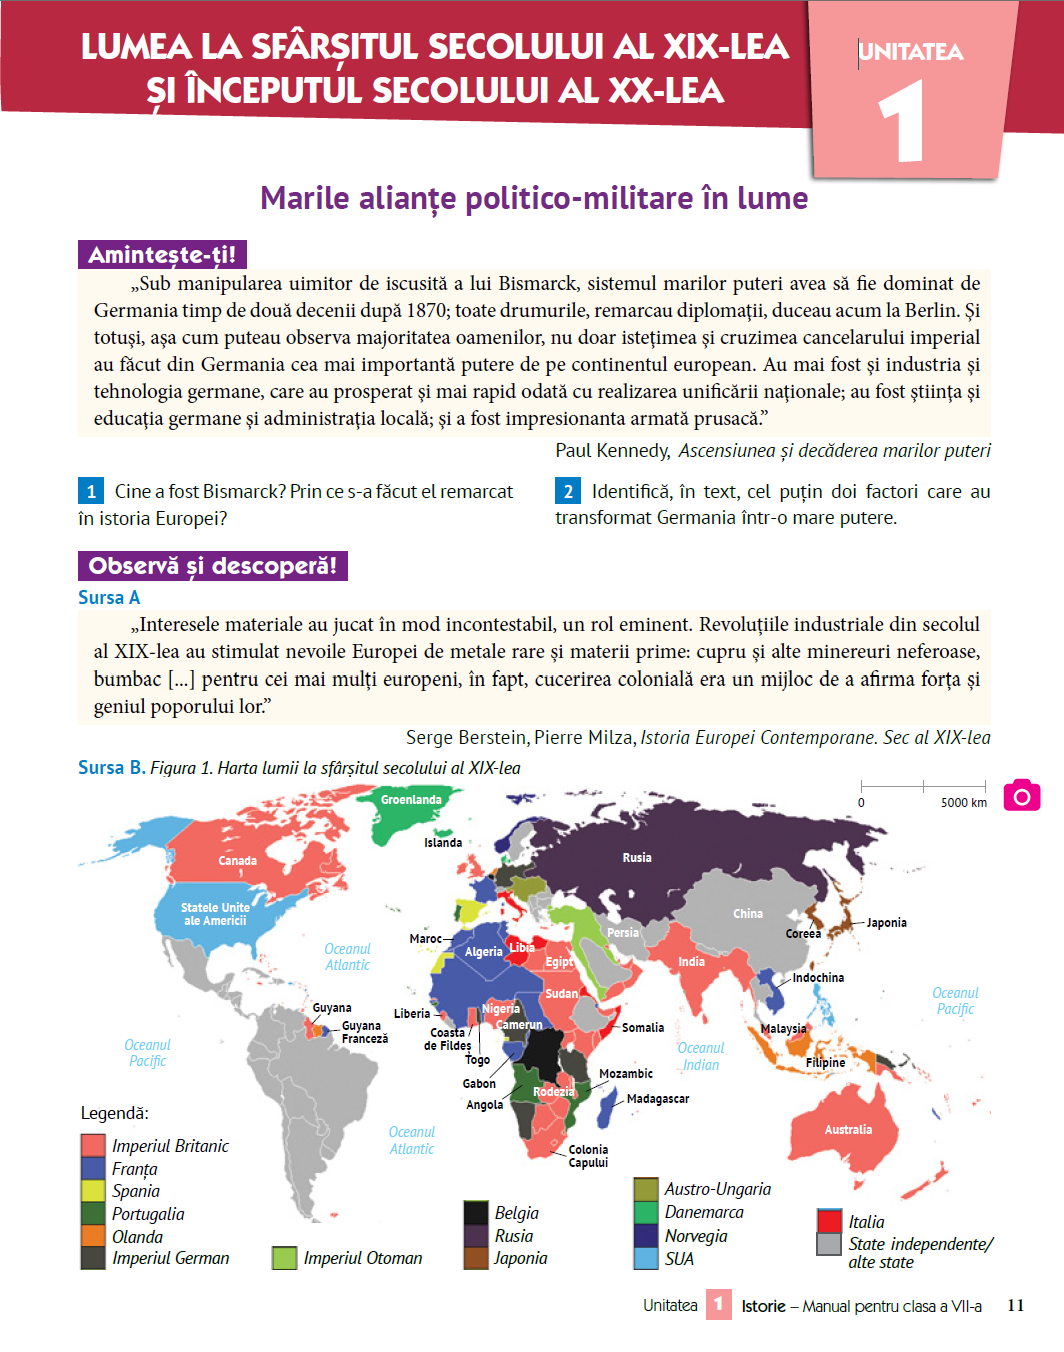
\includegraphics[width=.8\linewidth, height=.30\textheight]{Figura2_2a}
		\caption{pagină din manualul tipărit}
		\label{fig:Figura2_2a}
	\end{subfigure}%
	\begin{subfigure}{.5\textwidth}
		\centering
		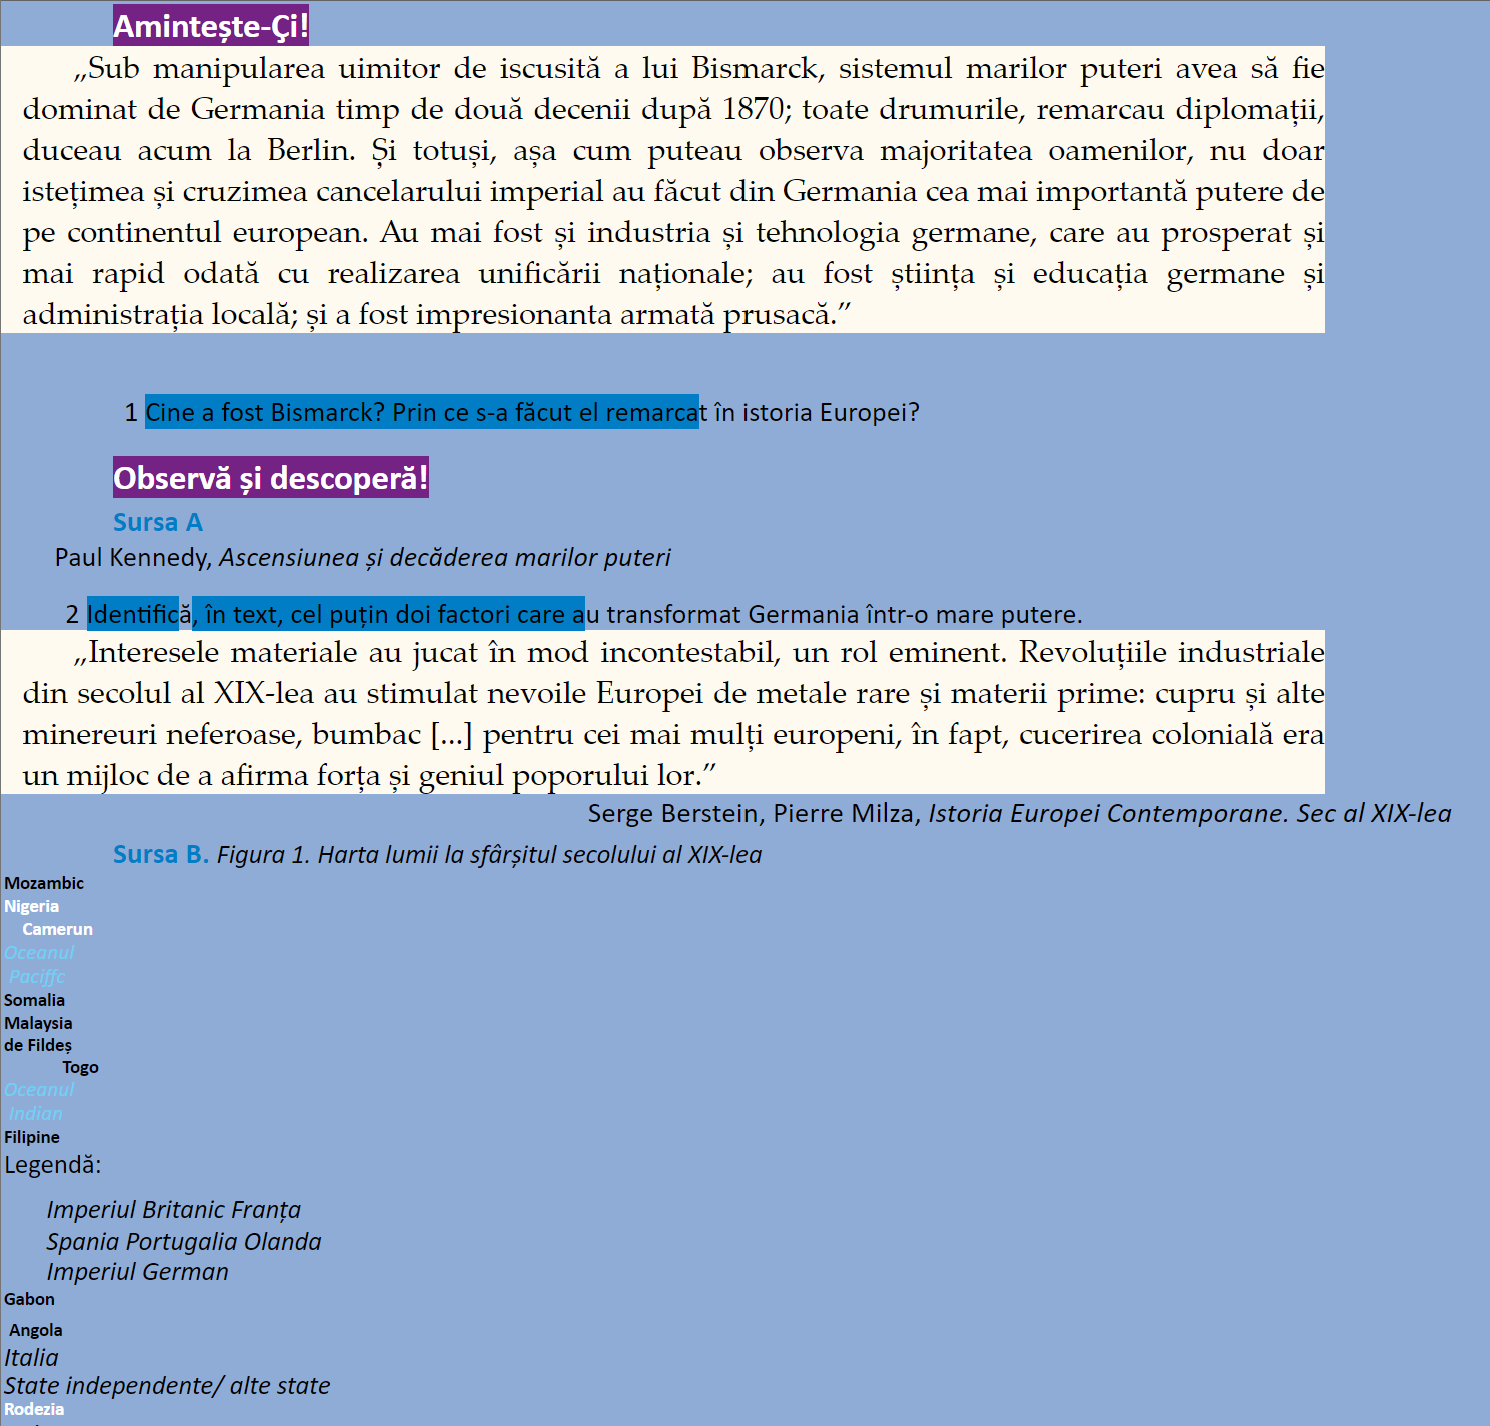
\includegraphics[width=.8\linewidth, height=.30\textheight]{Figura2_2b}
		\caption{pagină HTML generată de Xodo}
		\label{fig:Figura2_2b}
	\end{subfigure}
	\caption{Comparație de pagini dintre varianta tipărită și cea de la Xodo}
	\label{fig:Figura2_2}
\end{figure}

\noindent
Avantaje:
\begin{itemize}
	\item generează rapid pagini HTML;
	\item paginile sunt responsive;
	\item textul este selectabil.
\end{itemize}

\noindent
Dezavantaje:
\begin{itemize}
	\item limitat la o singură utilizare gratis pe zi;
	\item codul HTML este greu de editat;
	\item formatare greșită a textului.
\end{itemize}

\subsection{Soluția pdf2htmlEX}

O soluție care oferă o formatare ideală este obținută folosind pdf2htmlEX \cite{wang2013online}. Acest instrument păstrează tot textul și formatarea din PDF, dar are două dezavantaje. În primul rând, paginile rezultate nu sunt responsive, ceeea ce este o condiție obligatorie. O pagină responsive își păstrează structura atunci când este redimensionată. De exemplu, pagina HTML redimensionată pentru un ecran de telefon ar trebui să-și păstreze structura, ceea ce nu se întâmplă în cazul de față. Pe lângă acest lucru, codul HTML este greu de citit și de editat. O linie de cod poate să ajungă până la 60.000 de caractere. În cazul în care apar modificări în manual, acestea vor fi greu de editat.

Două dintre site-urile care folosesc acest instrument sunt CloudConvert și Convertio. Acestea dau rezultate asemănătoare, dar au amândouă aceleași probleme.
\begin{figure}[H]
	\centering
	\begin{subfigure}{.5\textwidth}
		\centering
		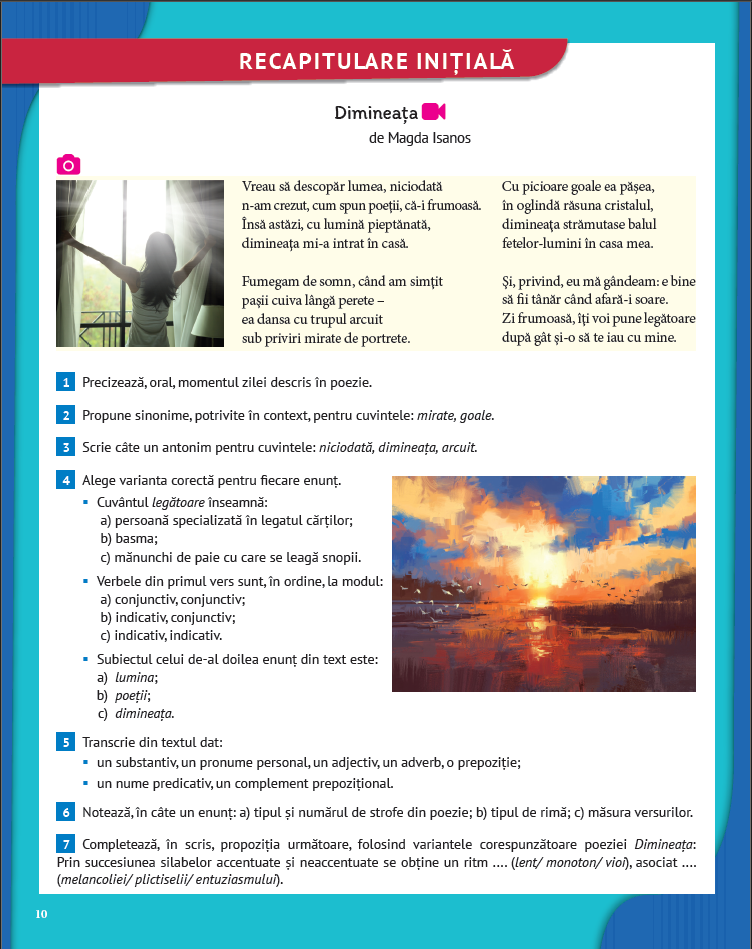
\includegraphics[width=.8\linewidth, height=.30\textheight]{Figura2_3a}
		\caption{pagină din manualul tipărit}
		\label{fig:Figura2_3a}
	\end{subfigure}%
	\begin{subfigure}{.5\textwidth}
		\centering
		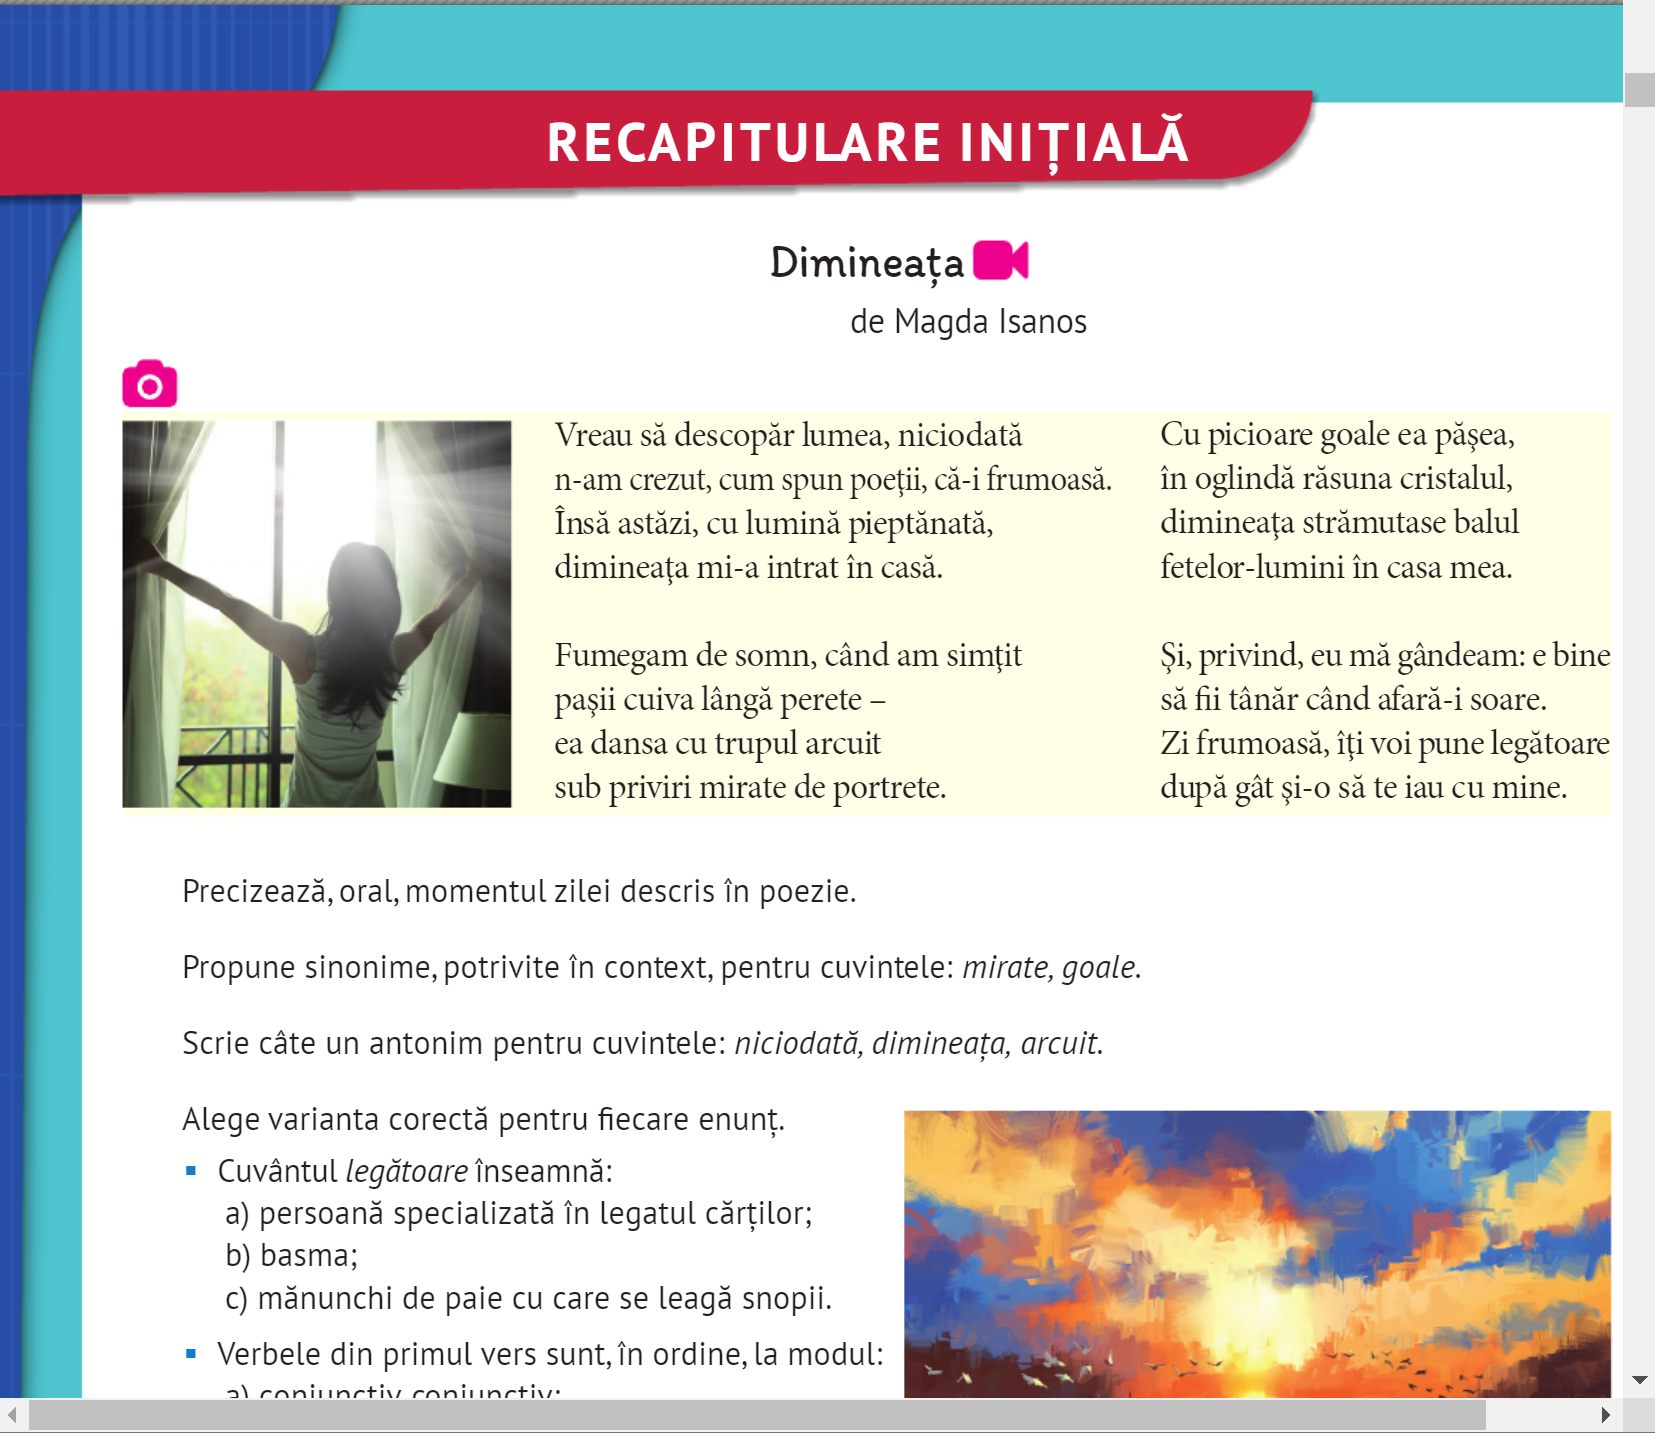
\includegraphics[width=.8\linewidth, height=.30\textheight]{Figura2_3b}
		\caption{pagină HTML generată de CloudConvert}
		\label{fig:Figura2_3b}
	\end{subfigure}
	\caption{Comparație de pagini dintre varianta tipărită și cea de la CloudConvert}
	\label{fig:Figura2_3}
\end{figure}

\noindent
Avantaje:
\begin{itemize}
	\item generează rapid pagini HTML;
	\item textul este selectabil;
	\item păstrează formatarea exact cum este în manualul tipărit;
	\item nu este limitat la un număr de utilizări.
\end{itemize}

\noindent
Dezavantaje:
\begin{itemize}
	\item paginile nu sunt responsive;
	\item codul HTML este greu de editat.
\end{itemize}

\section{HTML 4.01 Transitional}

O altă soluție găsită a fost extragerea textului din documentul PDF și plasarea acestuia într-un fișier de tip HTML 4.01 Transitional \cite{raggett1997html}. Deși acest format este mai simplu de utilizat și editat, el nu este la fel de modern ca HTML5.

Un exemplu de site care utilizează această metodă de conversie este PDF24 Tools. Avantajul principal este ușurința cu care se poate edita codul HTML. Totuși, site-ul nu păstrează formatul original al documentului PDF. Singurele atribute pe care le menține sunt stilurile de text bold și italic.
\begin{figure}[H]
	\centering
	\begin{subfigure}{.5\textwidth}
		\centering
		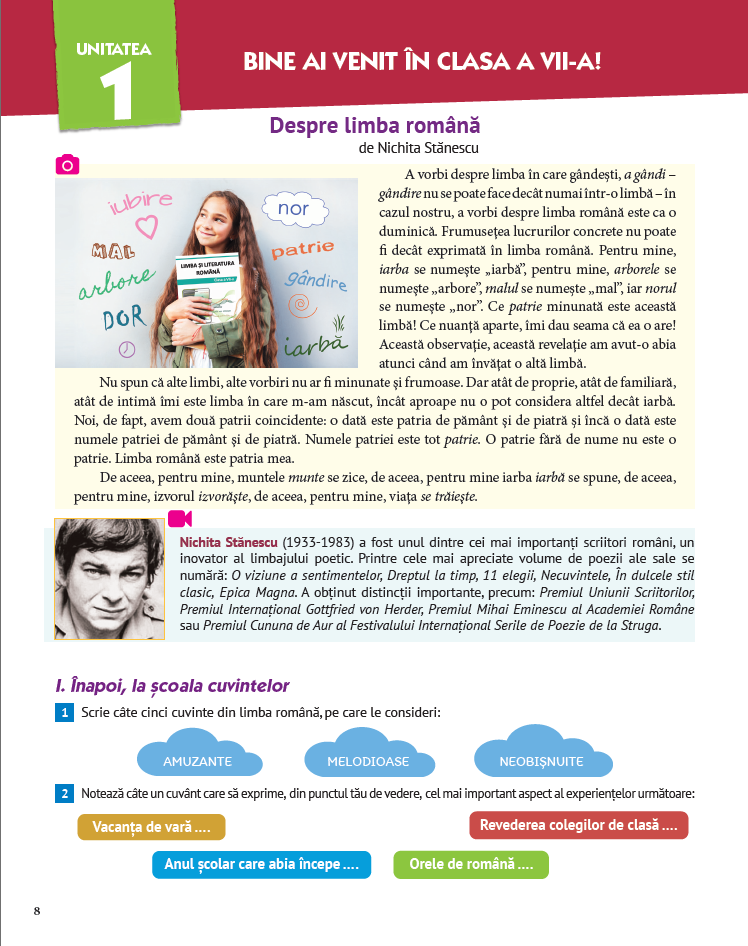
\includegraphics[width=.8\linewidth, height=.3\textheight]{Figura2_4a}
		\caption{pagină din manualul tipărit}
		\label{fig:Figura2_4a}
	\end{subfigure}%
	\begin{subfigure}{.5\textwidth}
		\centering
		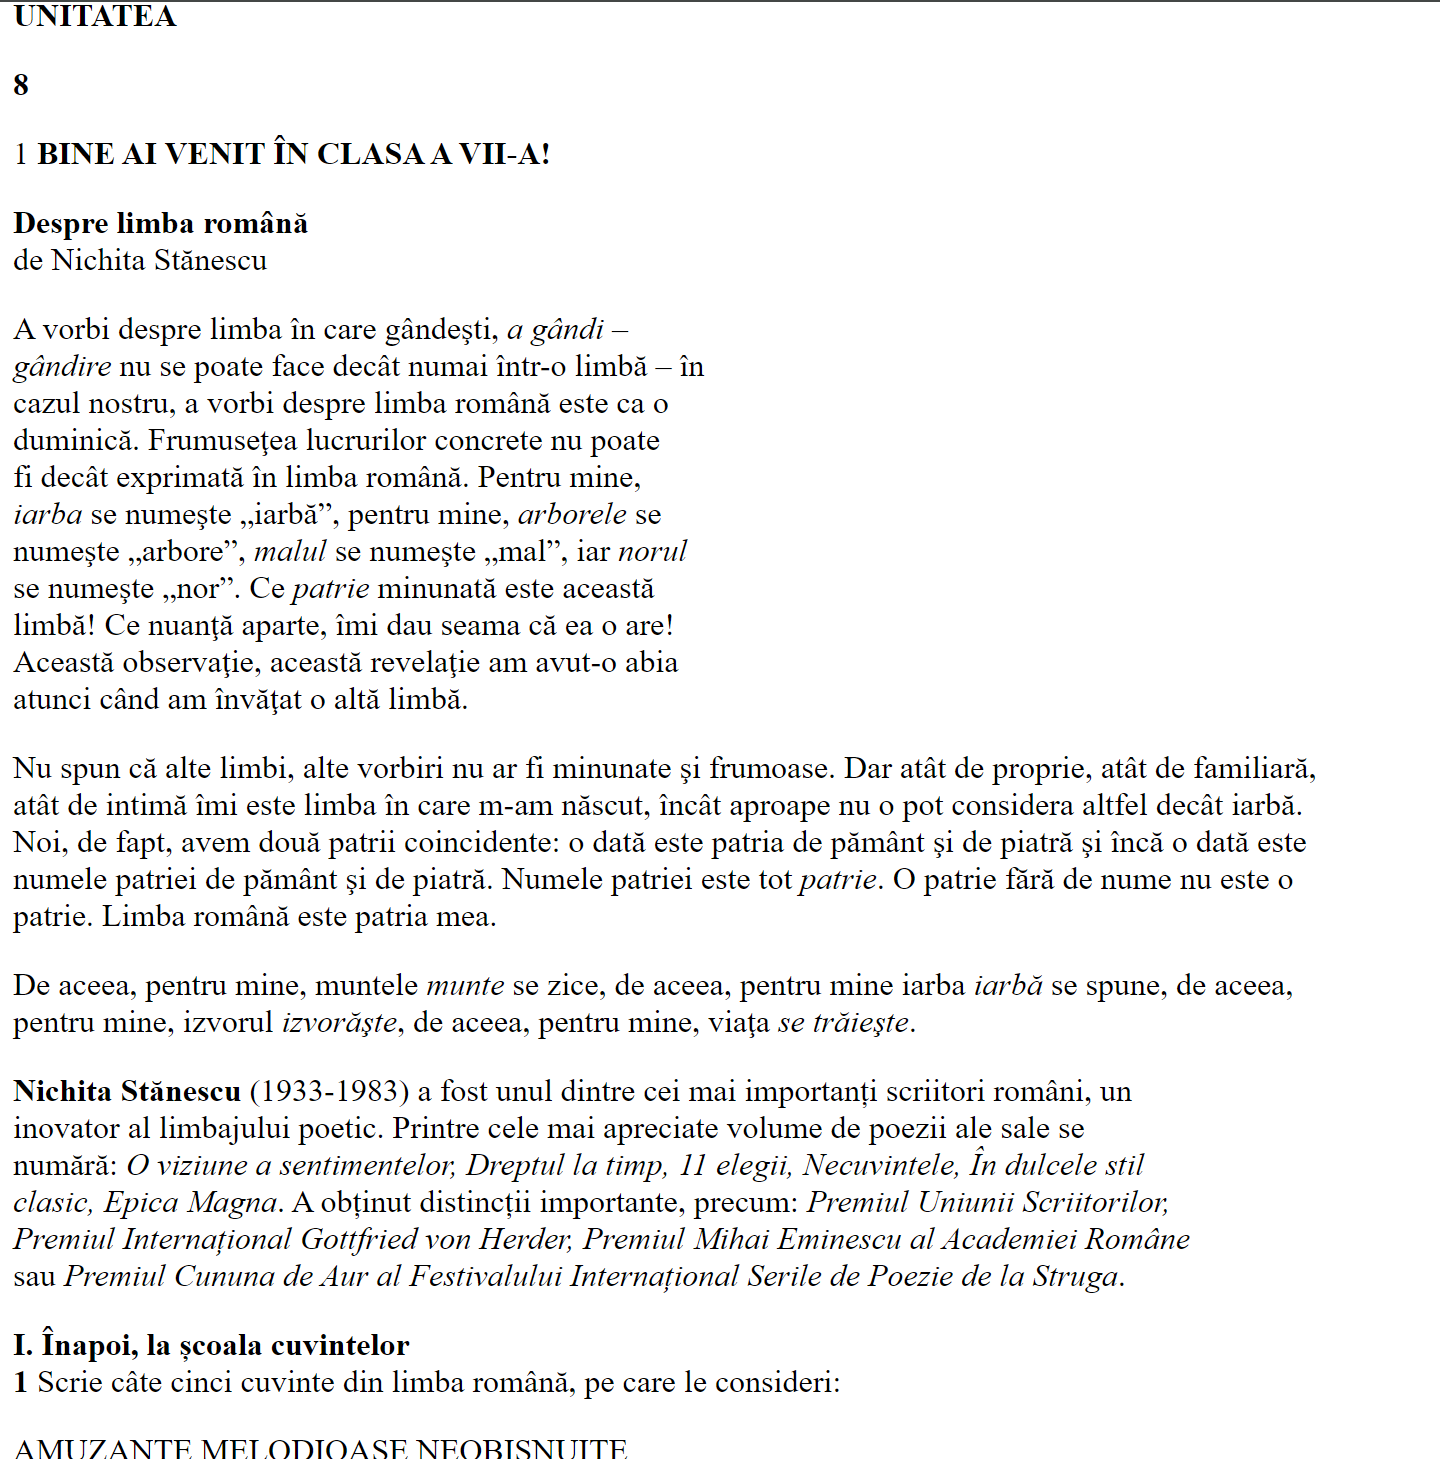
\includegraphics[width=.8\linewidth, height=.3\textheight]{Figura2_4b}
		\caption{pagină HTML generată de PDF24 Tools}
		\label{fig:Figura2_4b}
	\end{subfigure}
	\caption{Comparație de pagini dintre varianta tipărită și cea de la PDF24 Tools}
	\label{fig:Figura2_4}
\end{figure}

\noindent
Avantaje:
\begin{itemize}
	\item generează rapid pagini HTML;
	\item textul este selectabil;
	\item nu este limitat la un număr de utilizări;
	\item codul este ușor de editat.
\end{itemize}

\noindent
Dezavantaje:
\begin{itemize}
	\item păstrează doar o parte din formatarea originală (textul bold și italic).
\end{itemize}

\vspace{3em}
Necesitatea de a dezvolta încă un instrument de conversie a PDF-urilor în HTML provine din faptul că soluțiile actuale nu satisfac cerințele date de Minister. Niciuna dintre soluțiile analizate nu reprezintă un punct de plecare bun.

\begin{table}[H]
	\centering
	\begin{tabular}{| l | c | c | c | c |}
		\hline
		\textbf{Soluții/Criterii} & Selectabil & Responsive & Cod ușor de editat & Formatare corectă \\ \hline
		Conversia în imagini &  & $\times$ & $\times$ & $\times$ \\ \hline
		Xodo & $\times$ & $\times$ &  & \\ \hline
		pdf2htmlEX & $\times$ &  &  & $\times$ \\ \hline
		PDF24 Tools & $\times$ & $\times$ & $\times$ & \\ \hline
	\end{tabular}
	\caption{Comparație între instrumentele disponibile pe piață}
\end{table}
\chapter{Tehnologii folosite}
\section{Python}

Python este un limbaj de programare high-level, cunoscut pentru sintaxa sa clară și concisă \cite{van2006introduction}. A fost creat de Guido van Rossum în 1991. El este folosit pe scară largă, fiind renumit pentru aplicabilitatea lui în mai multe domenii. Printre acestea se numără dezvoltarea  web, data science, automatizarea și inteligența artificială.

Pentru crearea aplicațiilor de automatizare, Python reprezintă una dintre cele mai bune alegeri. Acest limbaj oferă mai multe avantaje deoarece prezintă o sintaxă intuitivă și o multitudine de librării, actualizate constant, care facilitează procesul de automatizare.


\section{Pip}

Pip este un manager de pachete pentru Python folosit pentru a instala și gestiona librării. Acesta permite instalarea ușoară a pachetelor din PyPI (Python Package Index) și are o sintaxă ușor de înțeles. Câteva comenzi de bază sunt:
\begin{itemize}
	\item \textbf{pip install <nume librărie>}: pentru a instala o librărie
	\item \textbf{pip uninstall <nume librărie>}: pentru a dezinstala o librărie
	\item \textbf{pip list}: pentru a afișa toate librăriile instalate
	\item \textbf{pip show <nume librărie>}: pentru a afișa mai multe informații despre o librărie
\end{itemize}


\section{PyMuPDF}

Una dintre provocările întâlnite a fost alegerea unei librării eficiente pentru manipularea documentelor PDF. Inițial, aplicația a fost dezvoltată folosind PyPDF2. Deși PyPDF2 este o librărie care manipulează documente în format PDF, aceasta s-a dovedit a fi prea lentă pentru volumul de manuale care trebuiau gestionate și nu oferea toate funcționalitățile necesare.

Pentru a depăși aceste limitări, a fost aleasă librăria PyMuPDF \cite{pymupdf}. Această librărie open-source oferă viteze mari pentru extragerea și scrierea infromațiilor din documente PDF. A fost inițial dezvoltată de Jorj X. McKie, iar ulterior a fost preluată de Artifex.

Pe lângă avantajele pe care le are această librărie în Python, PyMuPDF este disponibilă și în C și JavaScript. O diferență majoră între PyMuPDF și alte librării constă în faptul că celelalte librării sunt limitate doar la documente PDF, în timp ce PyMuPDF poate manipula o varietate de alte documente, cum ar fi XPS, EPUB, MOBI, FB2, CBZ, SVG, DOCX, XLSX și PPTX.

Conform site-ului oficial de la PyMuPDF \cite{pymupdf}, această librărie este una dintre cele mai rapide librării din Python pentru manipularea documentelor PDF. Drept dovadă, vor fi analizate cele mai importante funcționalități ale unei librării de acest fel: viteza de copiere, viteza de extragere și viteza de transformare a paginii într-o imagine.

Testele puse la dispoziție au fost realizate pe un set de 8 documente PDF cu un total de 7031 de pagini care conțin atât fragmente de text, cât și imagini.

Primul test măsoară viteza de citire si de rescriere a unui document PDF. Este un proces esențial pentru aplicațiile web ce permit combinarea mai multor documente PDF. Rezultatele testului sunt afișate în figura 3.1.
\begin{figure}[H]
	\centering
	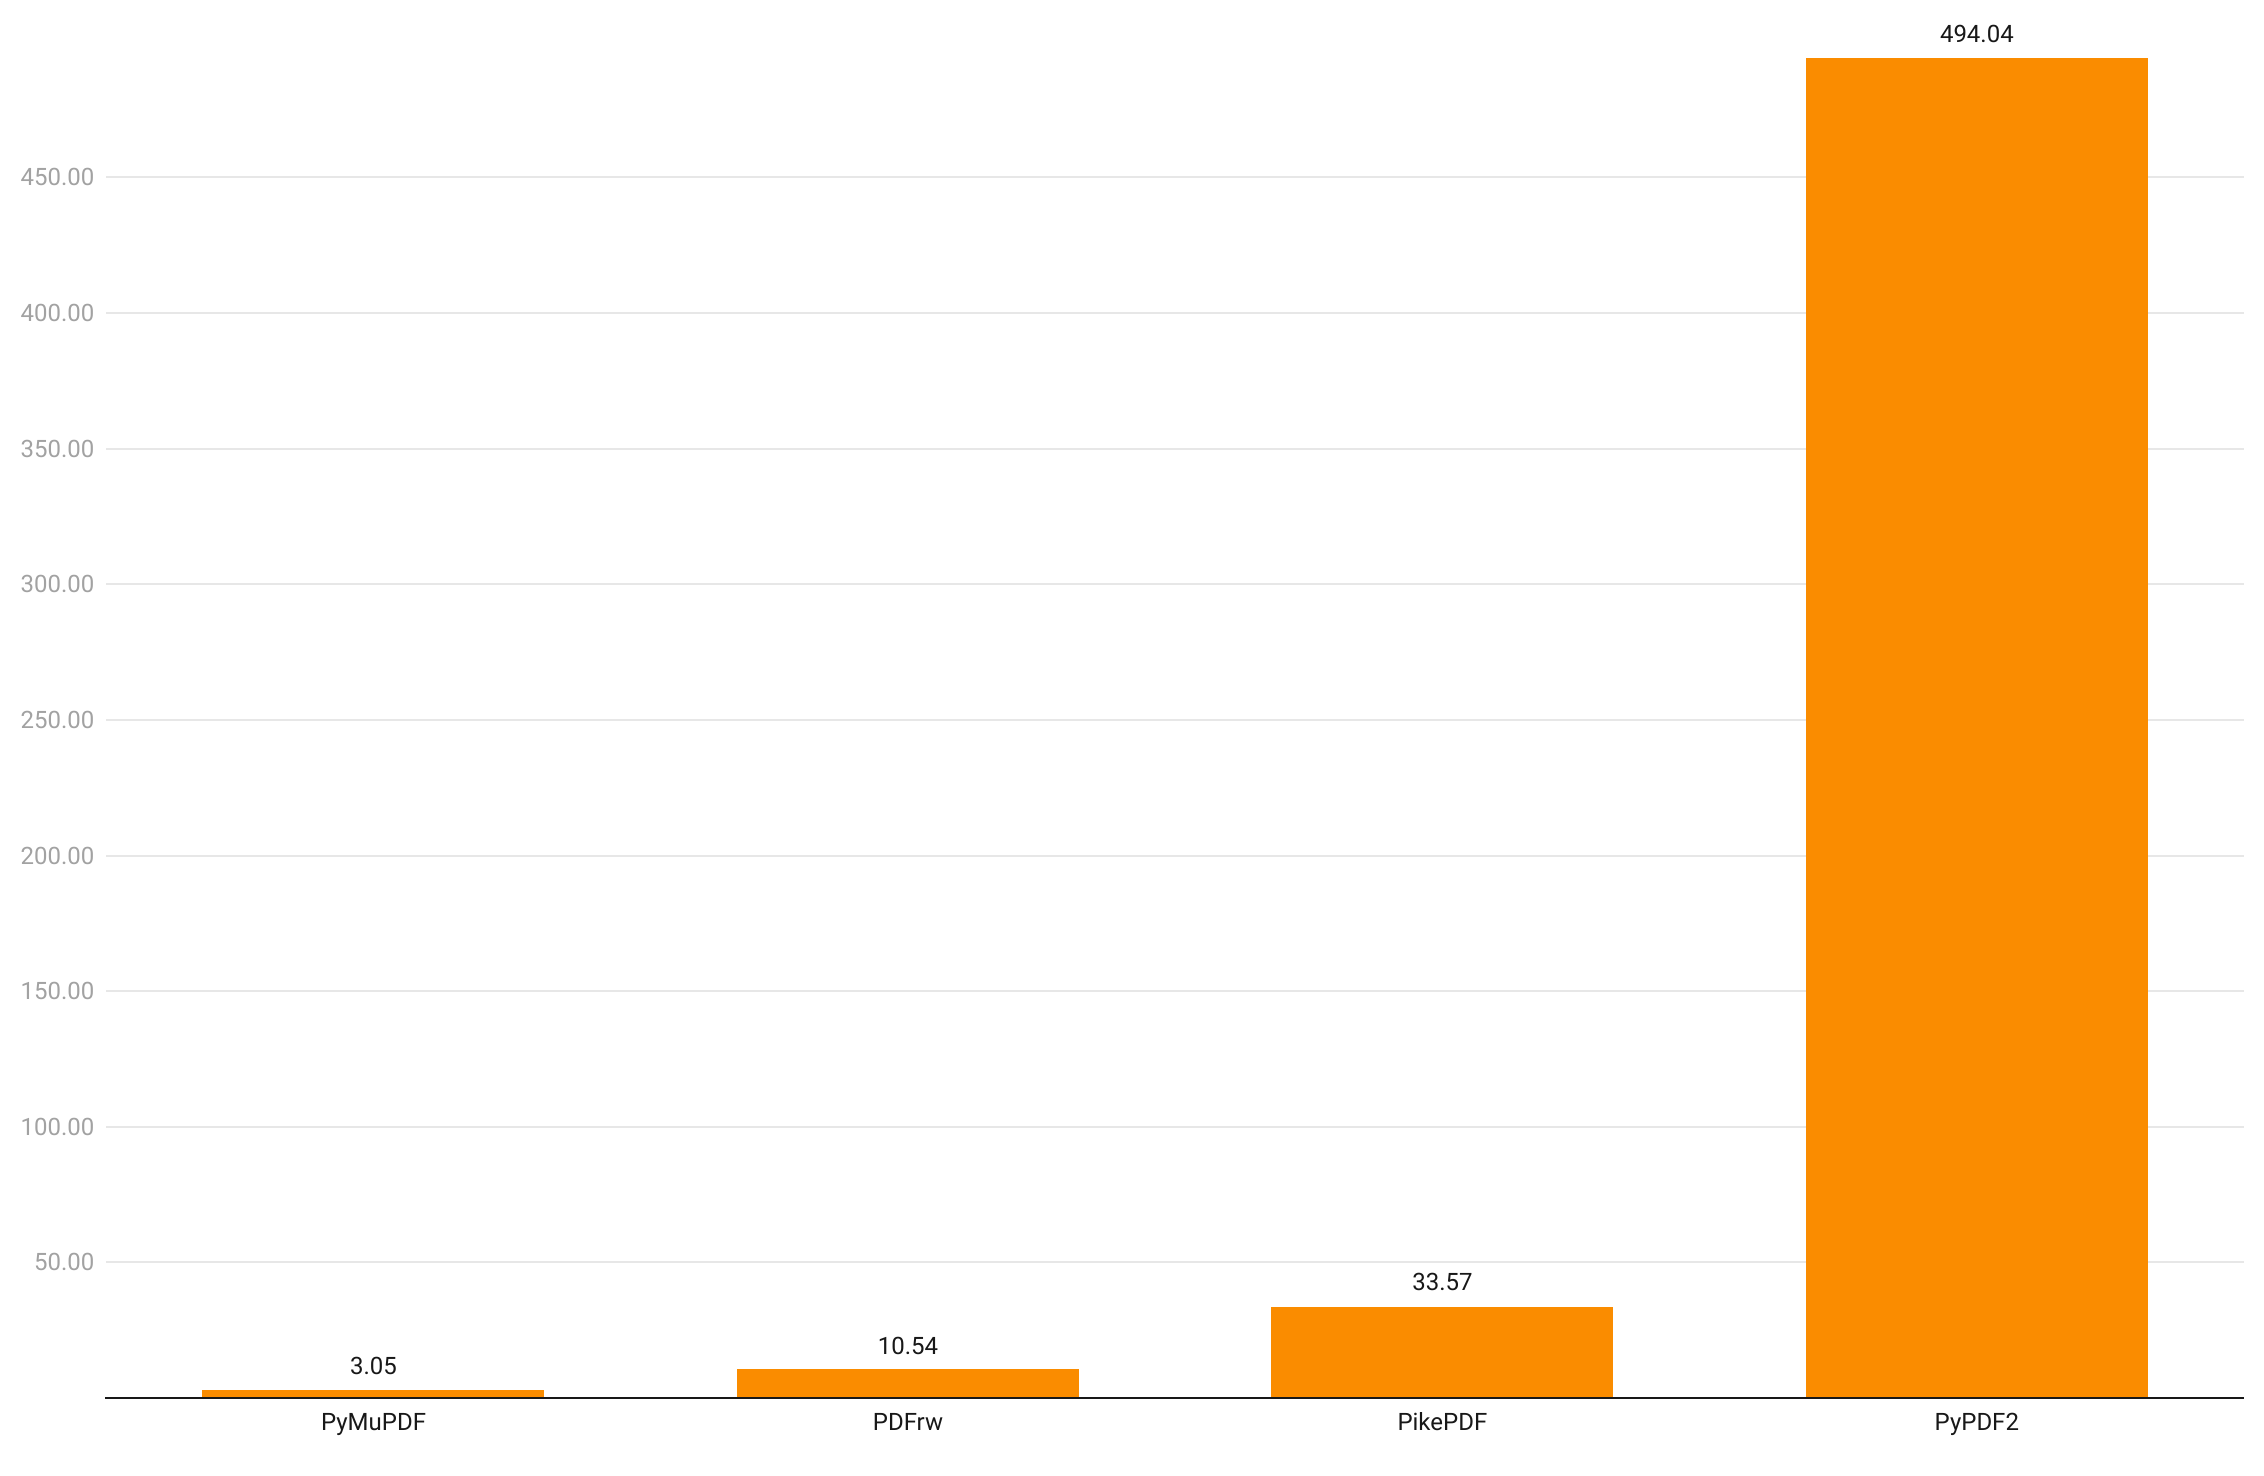
\includegraphics[scale=.25]{Figura3_1}
	\caption{Comparație de timp (în secunde) pentru copierea documentelor PDF}
	\label{fig:Figura3_1}
\end{figure}

Al doilea test măsoară durata procesului de extragere a unui text simplu dintr-un document PDF și scrierea lui într-un fișier .txt. Acest lucru este util pentru căutarea unui anumit termen din document sau pentru a efectua modificări în text. Rezultatele testului sunt afișate în figura 3.2.
\begin{figure}[H]
	\centering
	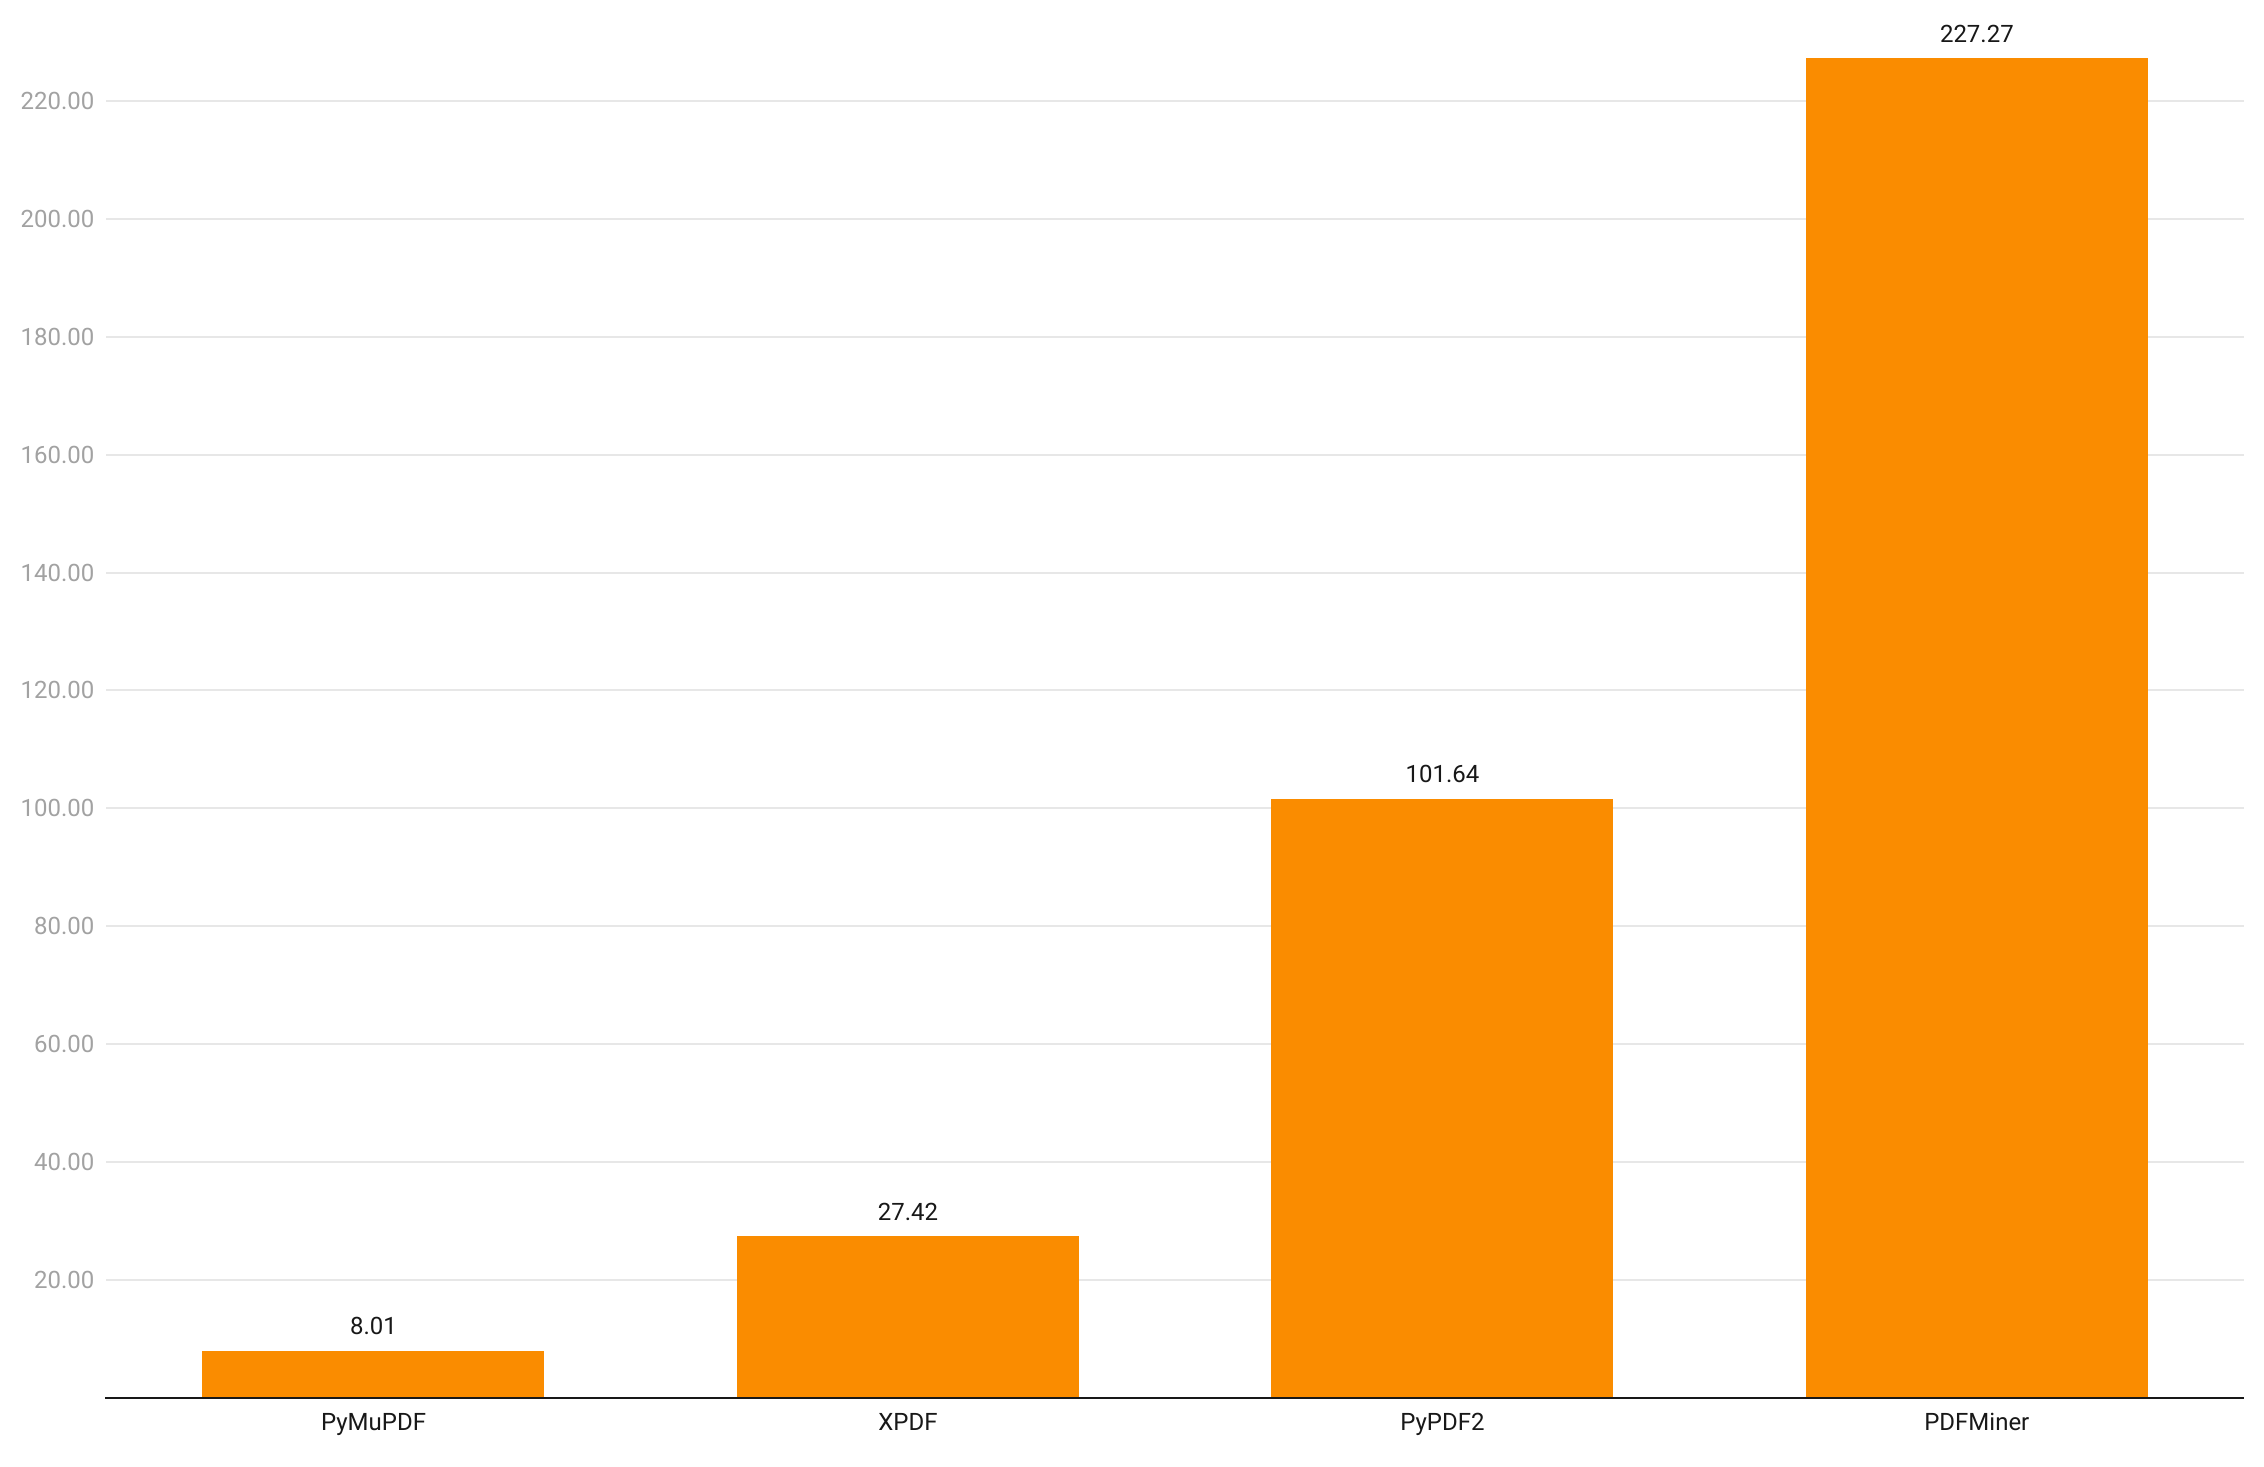
\includegraphics[scale=.25]{Figura3_2}
	\caption{Comparație de timp (în secunde) pentru extragerea textului din documente PDF}
	\label{fig:Figura3_2}
\end{figure}

Ultimul test măsoară viteza de transformare a documentelor PDF în imagini. Această funcționalitate este utilă atunci când se dorește afișarea paginilor din documentul PDF într-o interfață. Deschiderea unei imagini este mai rapidă decât deschiderea unui documentu. Rezultatele testului sunt afișate în figura 3.3.
\begin{figure}[H]
	\centering
	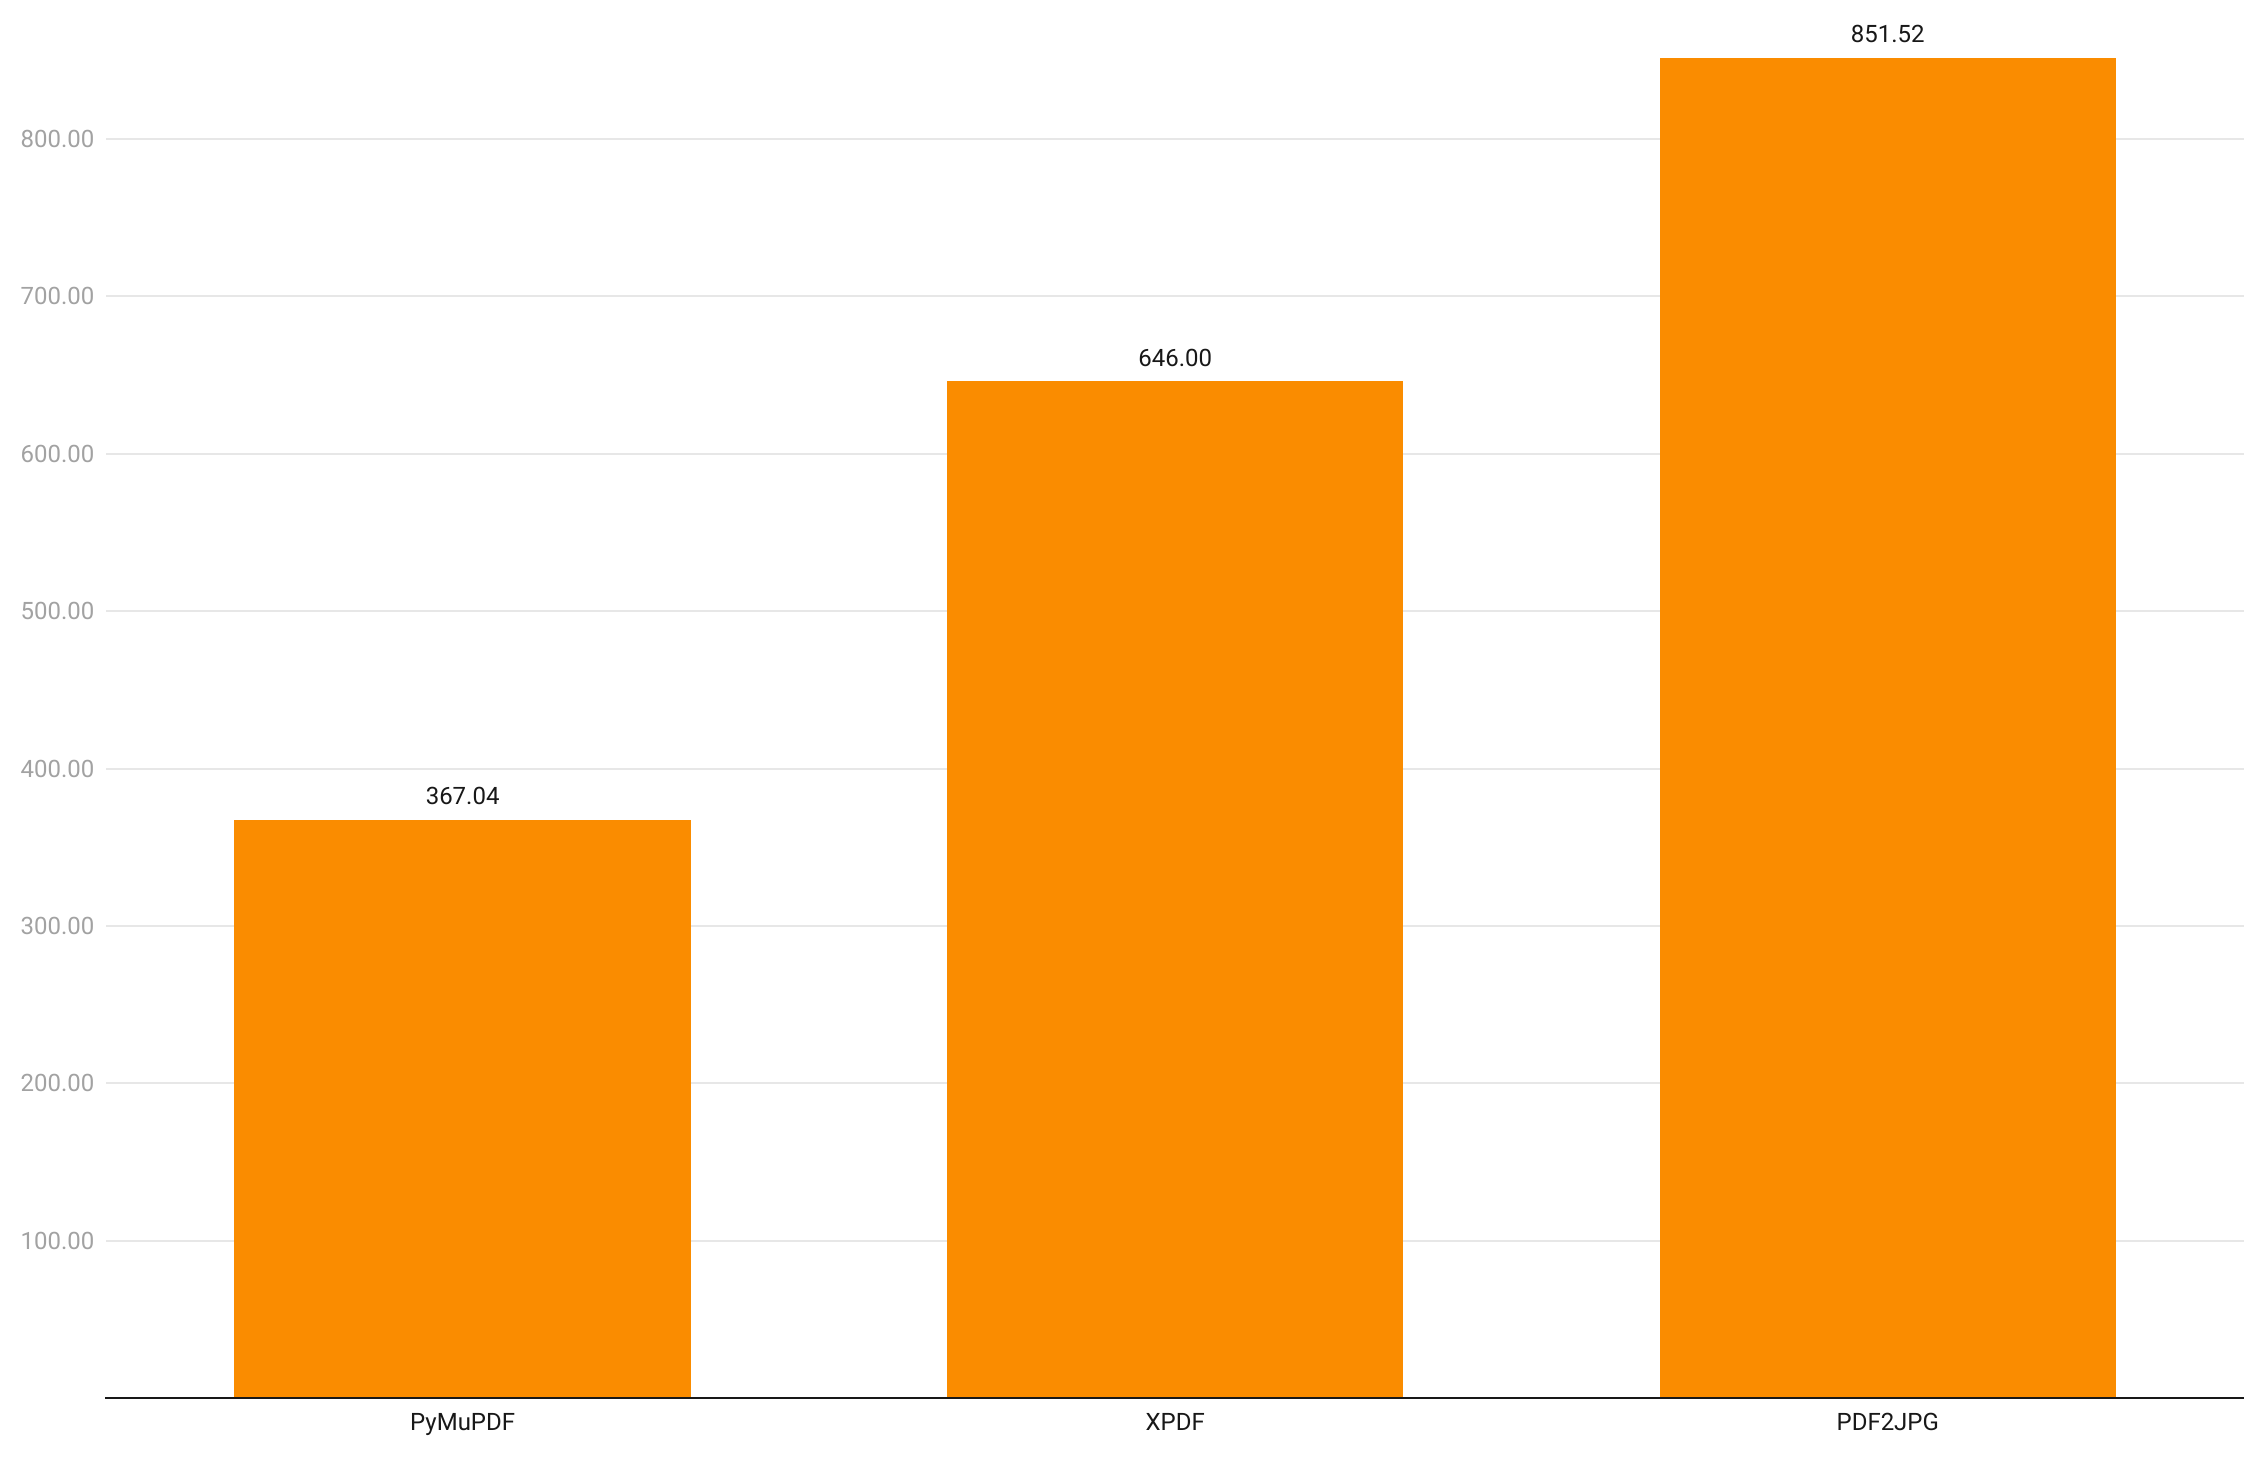
\includegraphics[scale=.2]{Figura3_3}
	\caption{Comparație de timp (în secunde) pentru transformarea paginilor în imagini}
	\label{fig:Figura3_3}
\end{figure}

Așa cum indică testele, PyMuPDF este o librărie de mare viteză care manipulează documente PDF. Pe lângă acest aspect, librăria oferă multe funcționalități și este constant actualizată. Din aceste motive, aplicația de automatizare va fi dezvoltată folosind PyMuPDF.


\section{MySQL}

MySQL \cite{dubois2013mysql} este un sistem de gestiune a bazelor de date (RDBMS). A fost lansat pe piață în anul 1995 de către MySQL AB. În anul 2008, compania a fost cumpărată de Sun Microsystems, iar aceștia în momentul de față fac parte din Oracle Corporation. MySQL este folosit de aplicații cunoscute precum: Facebook, Twitter, Netflix, Uber, Airbnb, Shopify.

Motivele principale pentru care a fost ales MySQL sunt ușurința integrării unei baze de date într-o aplicație dezvoltată în Python și viteza sa.  Rolul acestei baze de date în dezvoltarea aplicației de automatizare este de a stoca textul și metadatele din documentul PDF.





\chapter{Soluție propusă}
\section{Citire}

În acest subcapitol este prezentat modul de citire și stocare a metadatelor din manualul PDF. Procesul este împărțit în 3 etape: extragerea informațiilor de bază folosind PyMuPDF, asocierea unei culori de fundal pentru fiecare segment de text, extragerea imaginilor. Procesul se desfășoară conform următoarei diagrame.
\begin{figure}[H]
	\centering
	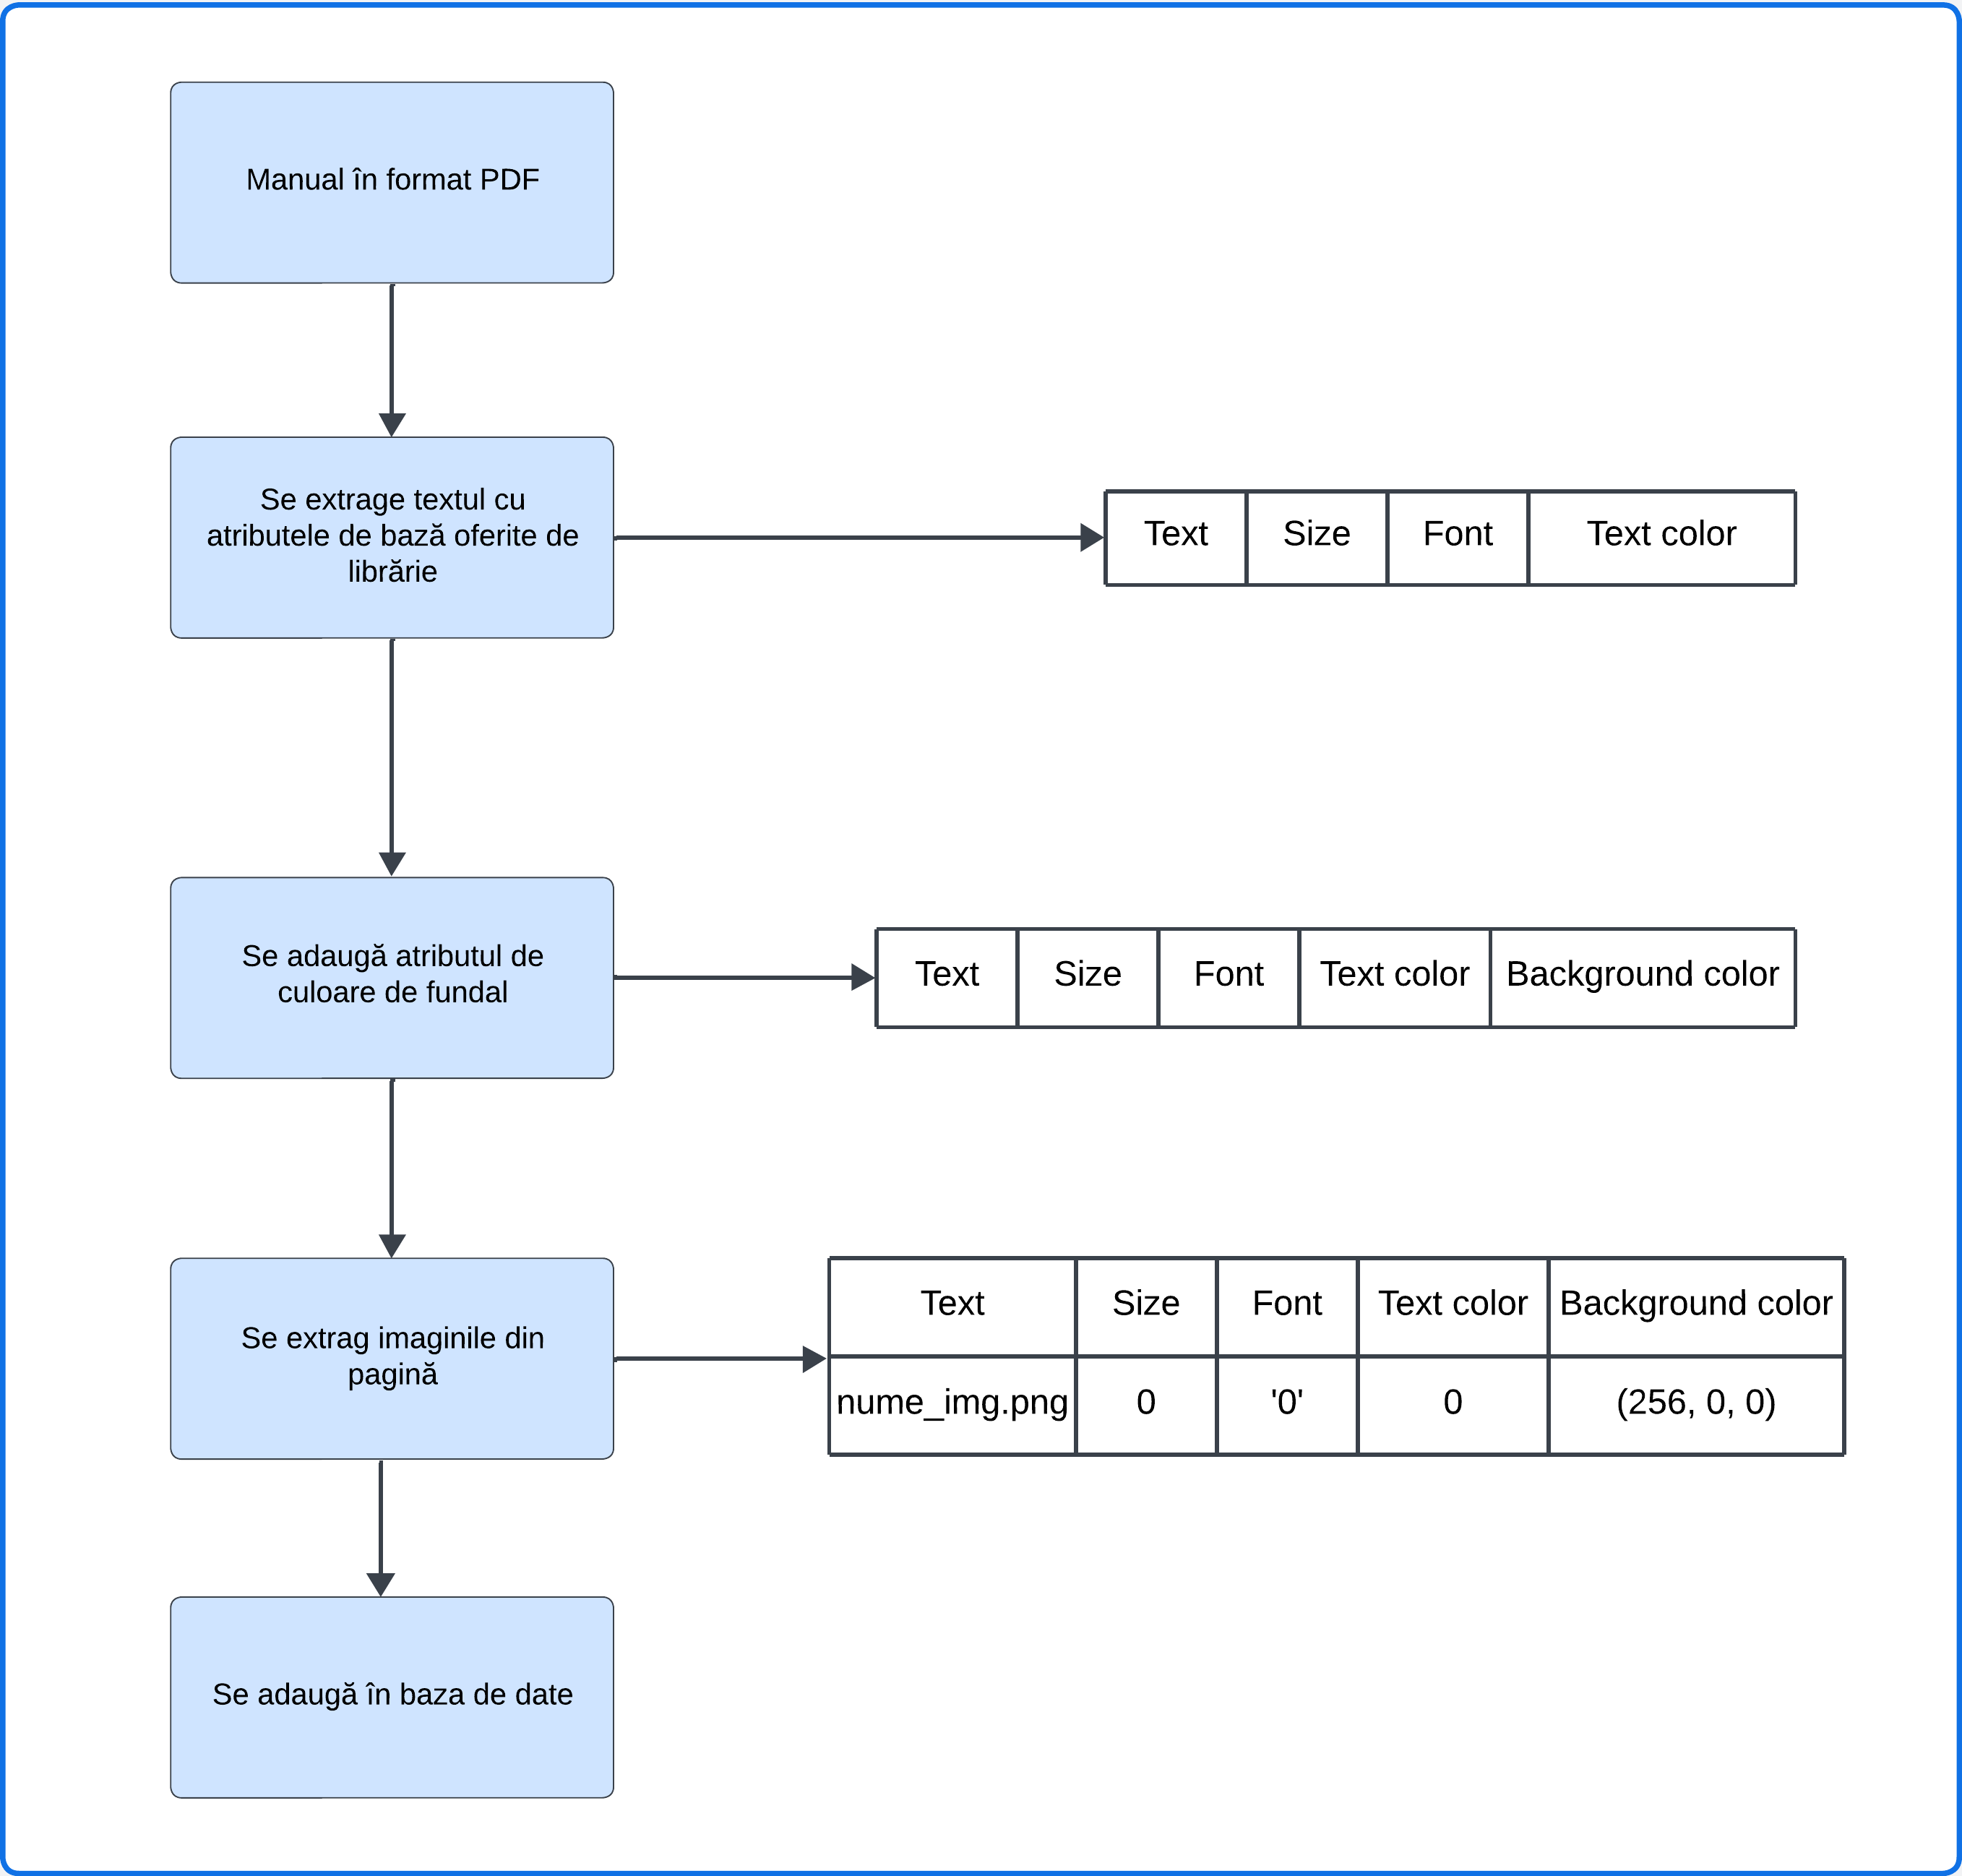
\includegraphics[scale=.5]{Figura4_1}
	\caption{Diagramă pentru subcapitolul de citire}
	\label{fig:Figura4_1}
\end{figure}

Pentru primul pas, se utilizează o funcție din librăria PyMuPDF care extrage majoritatea informațiilor importante despre documentul PDF. Această funcție extrage detalii precum culoarea textului, fontul, mărimea, coordonatele textului, dar și informații despre imagini cum ar fi tipul, lățimea, lungimea și transformările aplicate acestora.

Aceste informații sunt structurate ierarhic sub forma unor dicționare. Astfel, o pagină PDF conține un block, un block conține mai multe linii, iar o linie conține mai multe span-uri.
\begin{figure}[H]
	\centering
	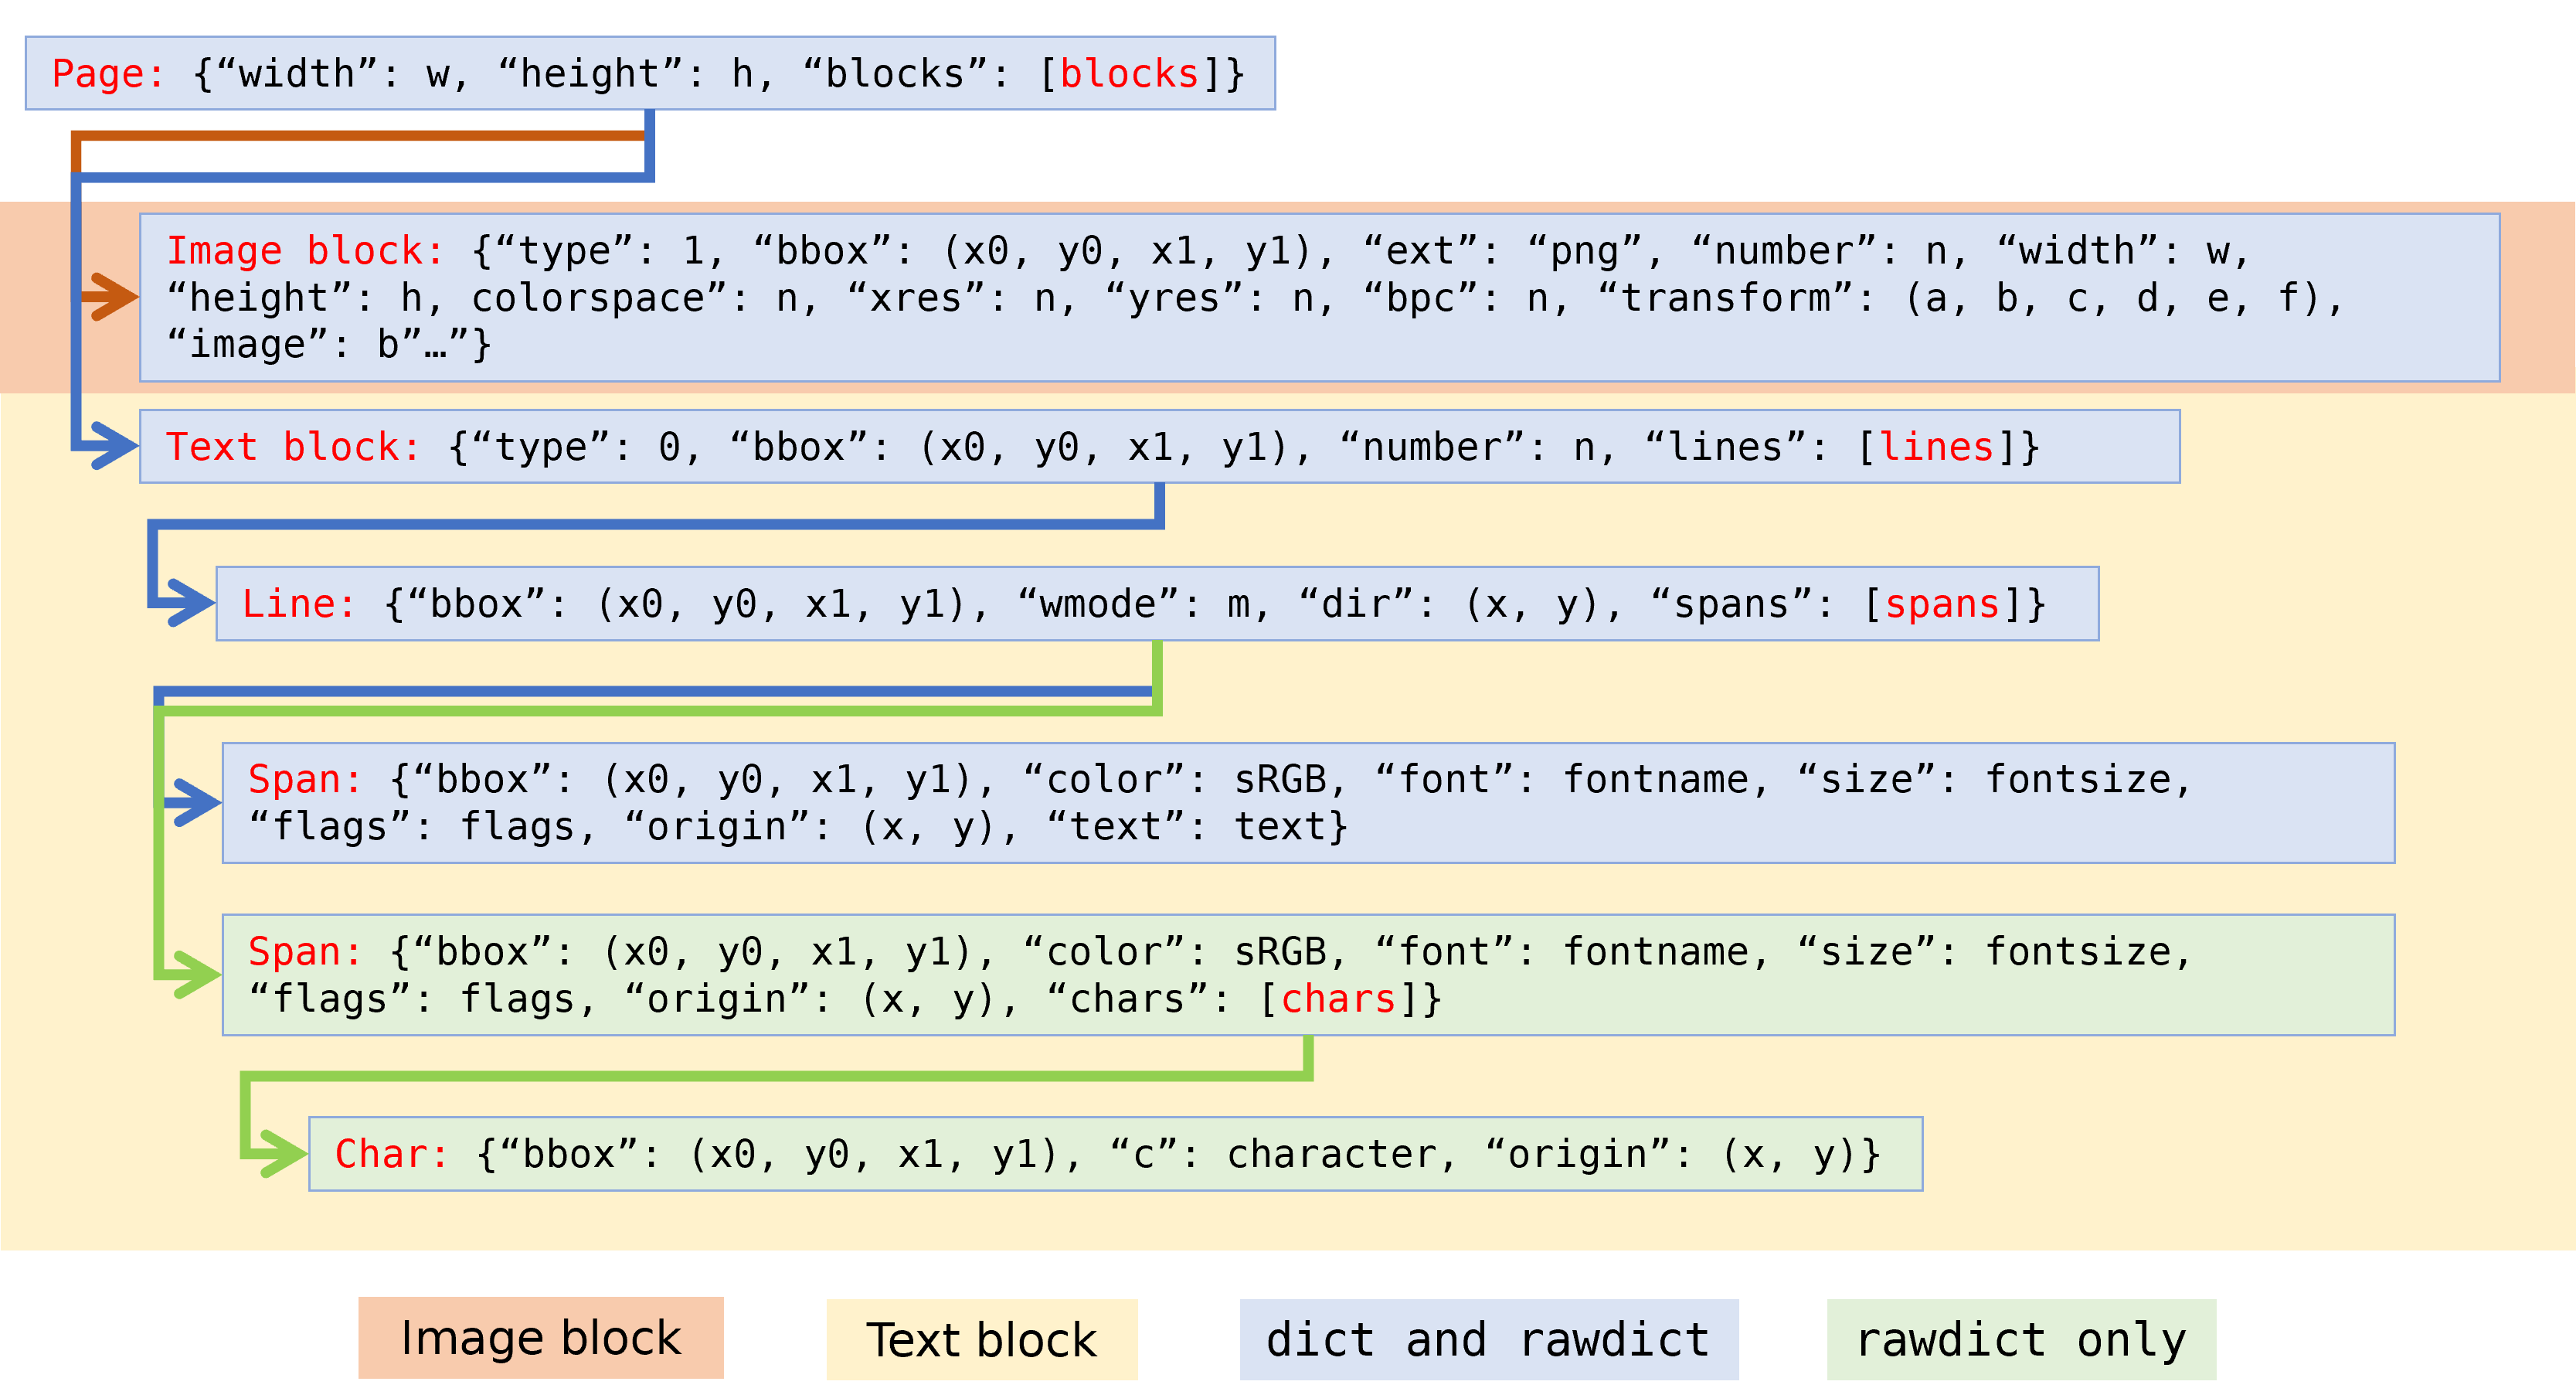
\includegraphics[scale=.15]{Figura4_2}
	\caption{Ierarhia informațiilor extrase din PDF}
	\label{fig:Figura4_2}
\end{figure}

Mărimea textului este măsurată în puncte (points), iar un punct reprezintă 1/72 inch. Pentru a extrage metadatele, se creează o funcție care va fi apelată la fiecare pagină. Aceasta va parcurge ierarhia pentru a obține informațiile necesare și pentru a le adăuga într-o listă de forma:
\begin{center}
	[Text, Size, Font, Text color]
\end{center}

\begin{lstlisting} [language=Python]
	def extract_pdf(path, page_nr):
		# Open PDF and extract text as a dictionary
		pdf = pymupdf.open(path)
		page = pdf.load_page(page_nr + 1)
		text_attributes_list = []
		text_attributes_dict = page.get_text('dict')
		
		for block in text_attributes_dict['blocks']:
			if block['type'] == 0:  # if type == 0 => text block
				for line in block['lines']:
					for span in line['spans']:
						text_attributes_list.append([span['text'], span['size'], 
						span['font'], span['color']])
			
		pdf.close()
		return text_attributes_list
\end{lstlisting}


\subsection{Culoarea de fundal}

Pentru a scrie textul în fișierul HTML final, este nevoie ca acesta să fie grupat în funcție de fragmentul din care face parte. Pentru unele porțiuni de text, singura metodă consistentă de grupare este cea bazată pe culoarea de fundal.

\vspace{3em}

În figura 4.3 este ilustrat un fragment de text cu fundal galben încadrat între două cerințe. Metodele de grupare implementate anterior nu au avut succes deoarece nu era clară delimitarea unui cu text cu fundal colorat de alte segmente de text. Astfel, a fost nevoie să se implementeze o metodă de determinare a culorii de fundal.
\begin{figure}[H]
	\centering
	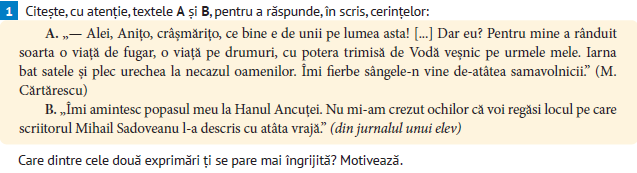
\includegraphics[scale=.8]{Figura4_3}
	\caption{Exemplu de text unde culoarea de fundal ajută la gruparea cuvintelor}
	\label{fig:Figura4_3}
\end{figure}

Pentru a extrage culoarea de fundal se va crea o funcție care verifică ce culoare apare predominant într-un block de text. Pașii urmați pentru a obține culoarea de fundal sunt:

\begin{itemize}
	\item transformarea paginii PDF într-un pixmap și ulterior într-o imagine;
	\item identificarea coordonatelor de la bounding box-urile fiecărei porțiune de text;
	\item determinarea celei mai frecvente culori din fiecare bounding box.
\end{itemize}

Pixmap-urile (pixel maps) sunt obiecte care stau la baza librăriei PyMuPDF. Ele reprezintă o suprafață cu un set de pixeli. Fiecare pixel este definit printr-un număr de bytes care reprezintă culoarea și transparența.

Bounding box-urile sunt chenare în care sunt încadrate block-urile de text. Acestea sunt prescurtate prin "bbox".

Înainte de a transforma pagina într-o imagine, este nevoie să o transformăm într-un pixmap. Acest lucru se face utilizând o funcție din librărie, căreia îi furnizăm o matrice de transformare. Această matrice modifică dimensiunile și înclinarea pixmap-urilor după cum urmează:
\begin{center}
	$\begin{bmatrix}
		a & b & 0\\
		c & d & 0\\
		e & f & 1
	\end{bmatrix}$
\end{center}

\noindent
Legendă coeficienți:
\begin{itemize}
	\item \(a\) - coeficient pentru a mări sau micșora lățimea (dacă este introdusă o valoare negativă, atunci poza se va întoarce invers de la stânga la dreapta).
	\item \(b\) - coeficient pentru a înclina imaginile orizontal; punctele de coordonate $A(x, y)$ vor deveni $A(x, y-b \cdot x)$.
	\item \(c\) - coeficient pentru a înclina imaginile vertical; punctele de coordonate $A(x, y)$ vor deveni $A(x - c \cdot y, y)$.
	\item \(d\) - coeficient pentru a mări sau micșora înălțimea (dacă este introdusă o valoare negativă, atunci poza se va întoarce invers de sus în jos).
	\item \(e\) - coeficient pentru a translata imaginea la stânga sau la dreapta; punctele de coordonate $A(x, y)$ vor deveni $A(x + e, y)$.
	\item \(f\) - coeficient pentru a translata imaginea mai sus sau mai jos; punctele de coordonate $A(x, y)$ vor deveni $A(x, y-f)$.
\end{itemize}

Exemplu de imagini pentru $b$ și $c$  modificat:
\begin{figure}[H]
	\centering
	\begin{subfigure}[t]{.5\textwidth}
		\centering
		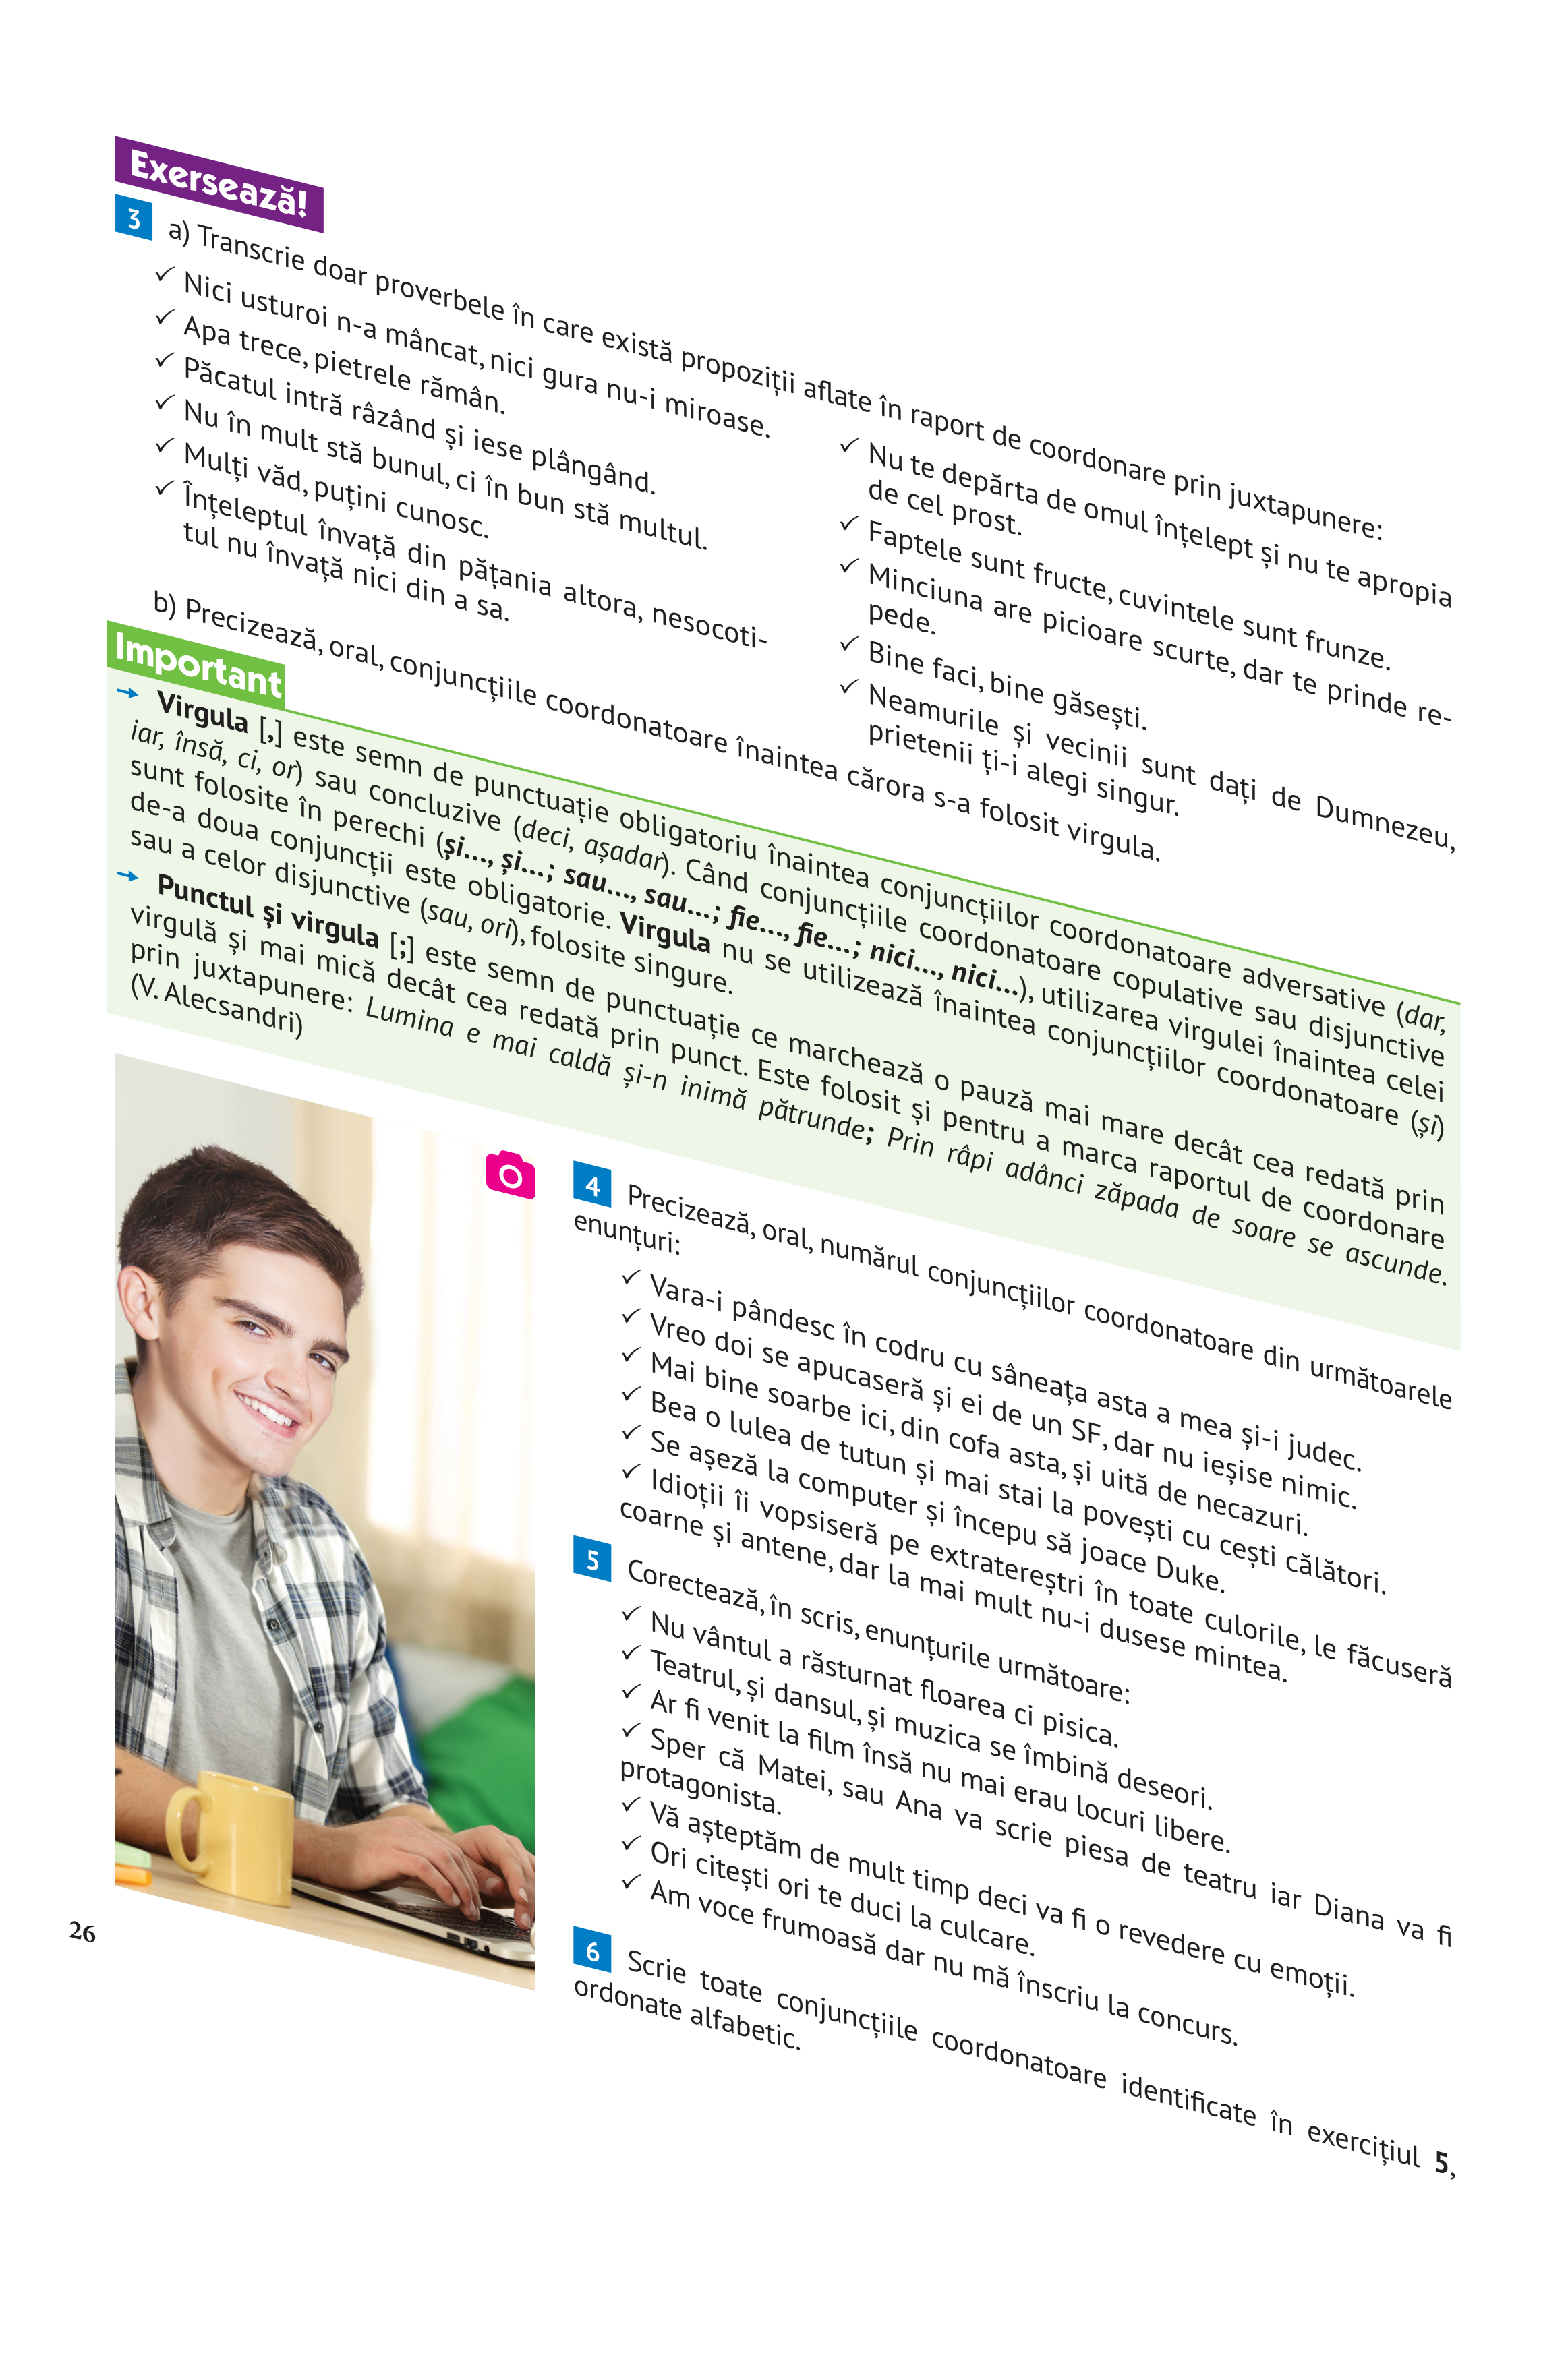
\includegraphics[width=.8\linewidth, height=.3\textheight]{Figura4_4a}
		\caption{Înclinare orizontală:
			$
			\begin{bmatrix}
				3 & 1 & 0\\
				0 & 3 & 0\\
				0 & 0 & 1
			\end{bmatrix}
			$}
		\label{fig:Figura4_4a}
	\end{subfigure}%
	\begin{subfigure}[t]{.5\textwidth}
		\centering
		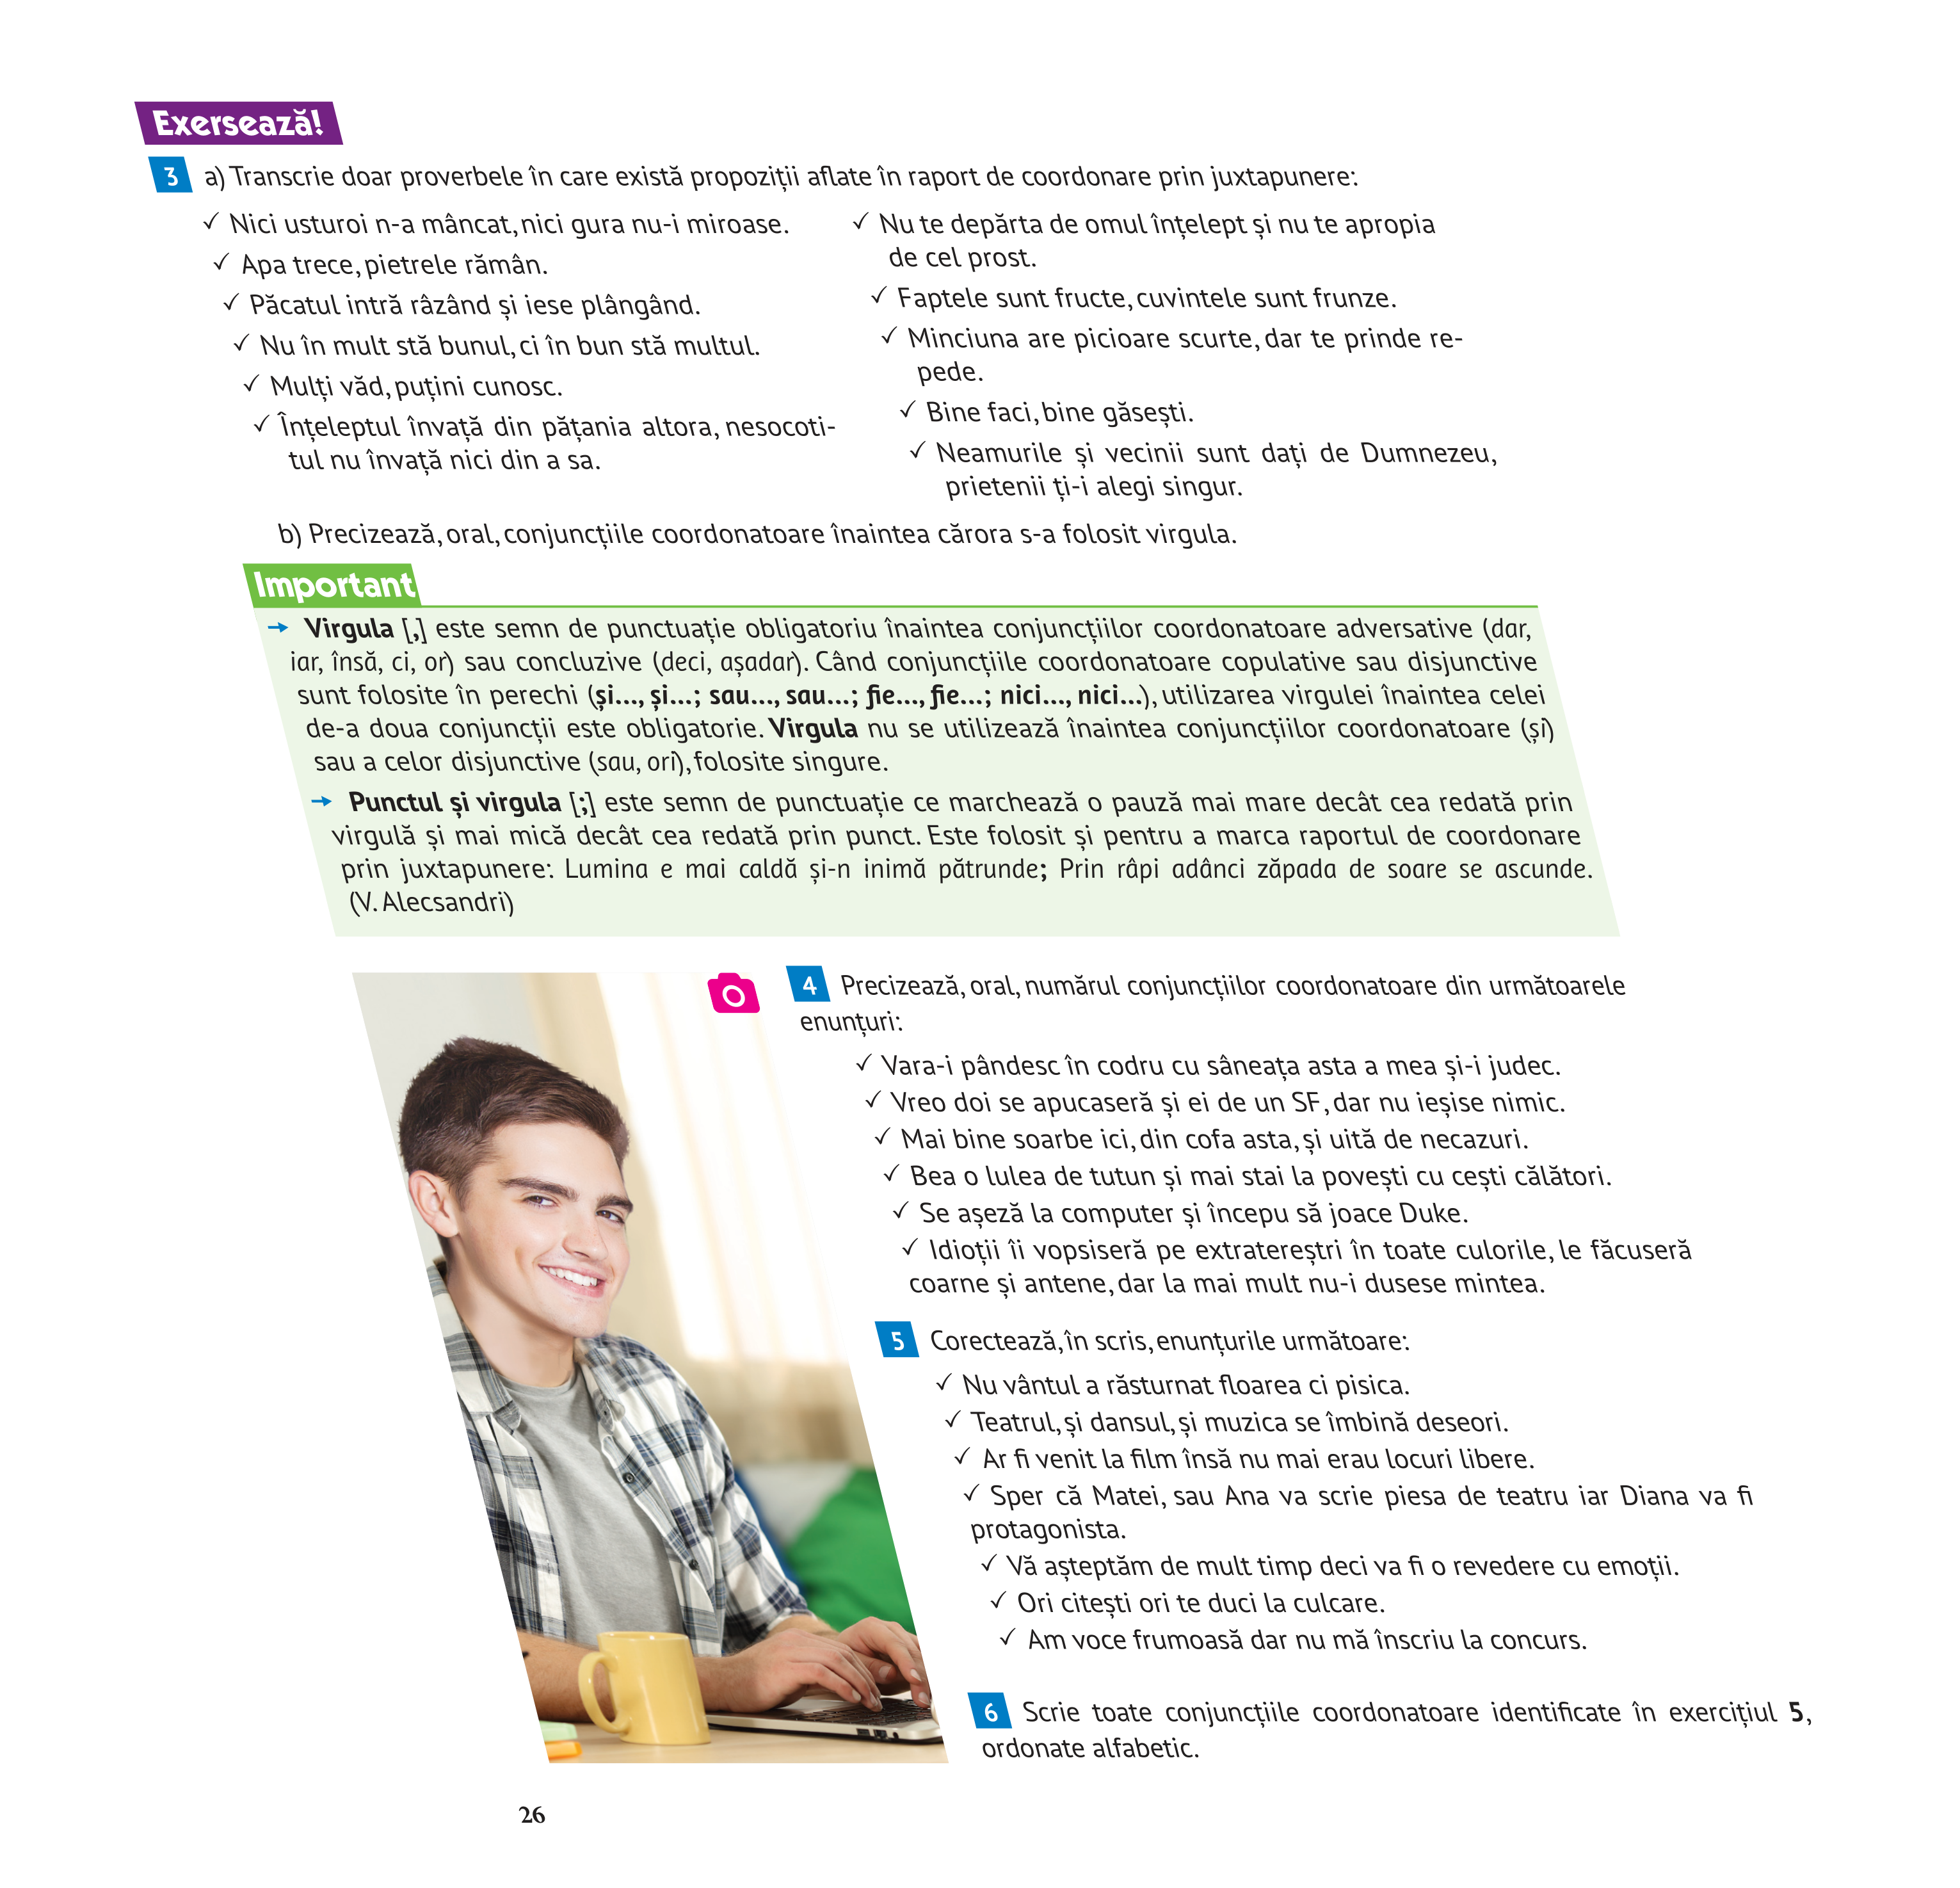
\includegraphics[width=.8\linewidth, height=.3\textheight]{Figura4_4b}
		\caption{Înclinare verticală:
			$
			\begin{bmatrix}
				3 & 0 & 0\\
				1 & 3 & 0\\
				0 & 0 & 1
			\end{bmatrix}
			$}
		\label{fig:Figura4_4b}
	\end{subfigure}
	\caption{Proprietăți ale matricii de transformare a imaginii}
	\label{fig:Figura4_4}
\end{figure}

Coeficienții care modifică rezoluția imaginii sunt $a$ și $d$. Aceștia sunt utilizați pentru a încadra textul cât mai precis posibil. Totuși, dacă se aleg valori prea mari, aplicația va rula mai lent din cauza rezoluției crescute.

\begin{figure}[H]
	\centering
	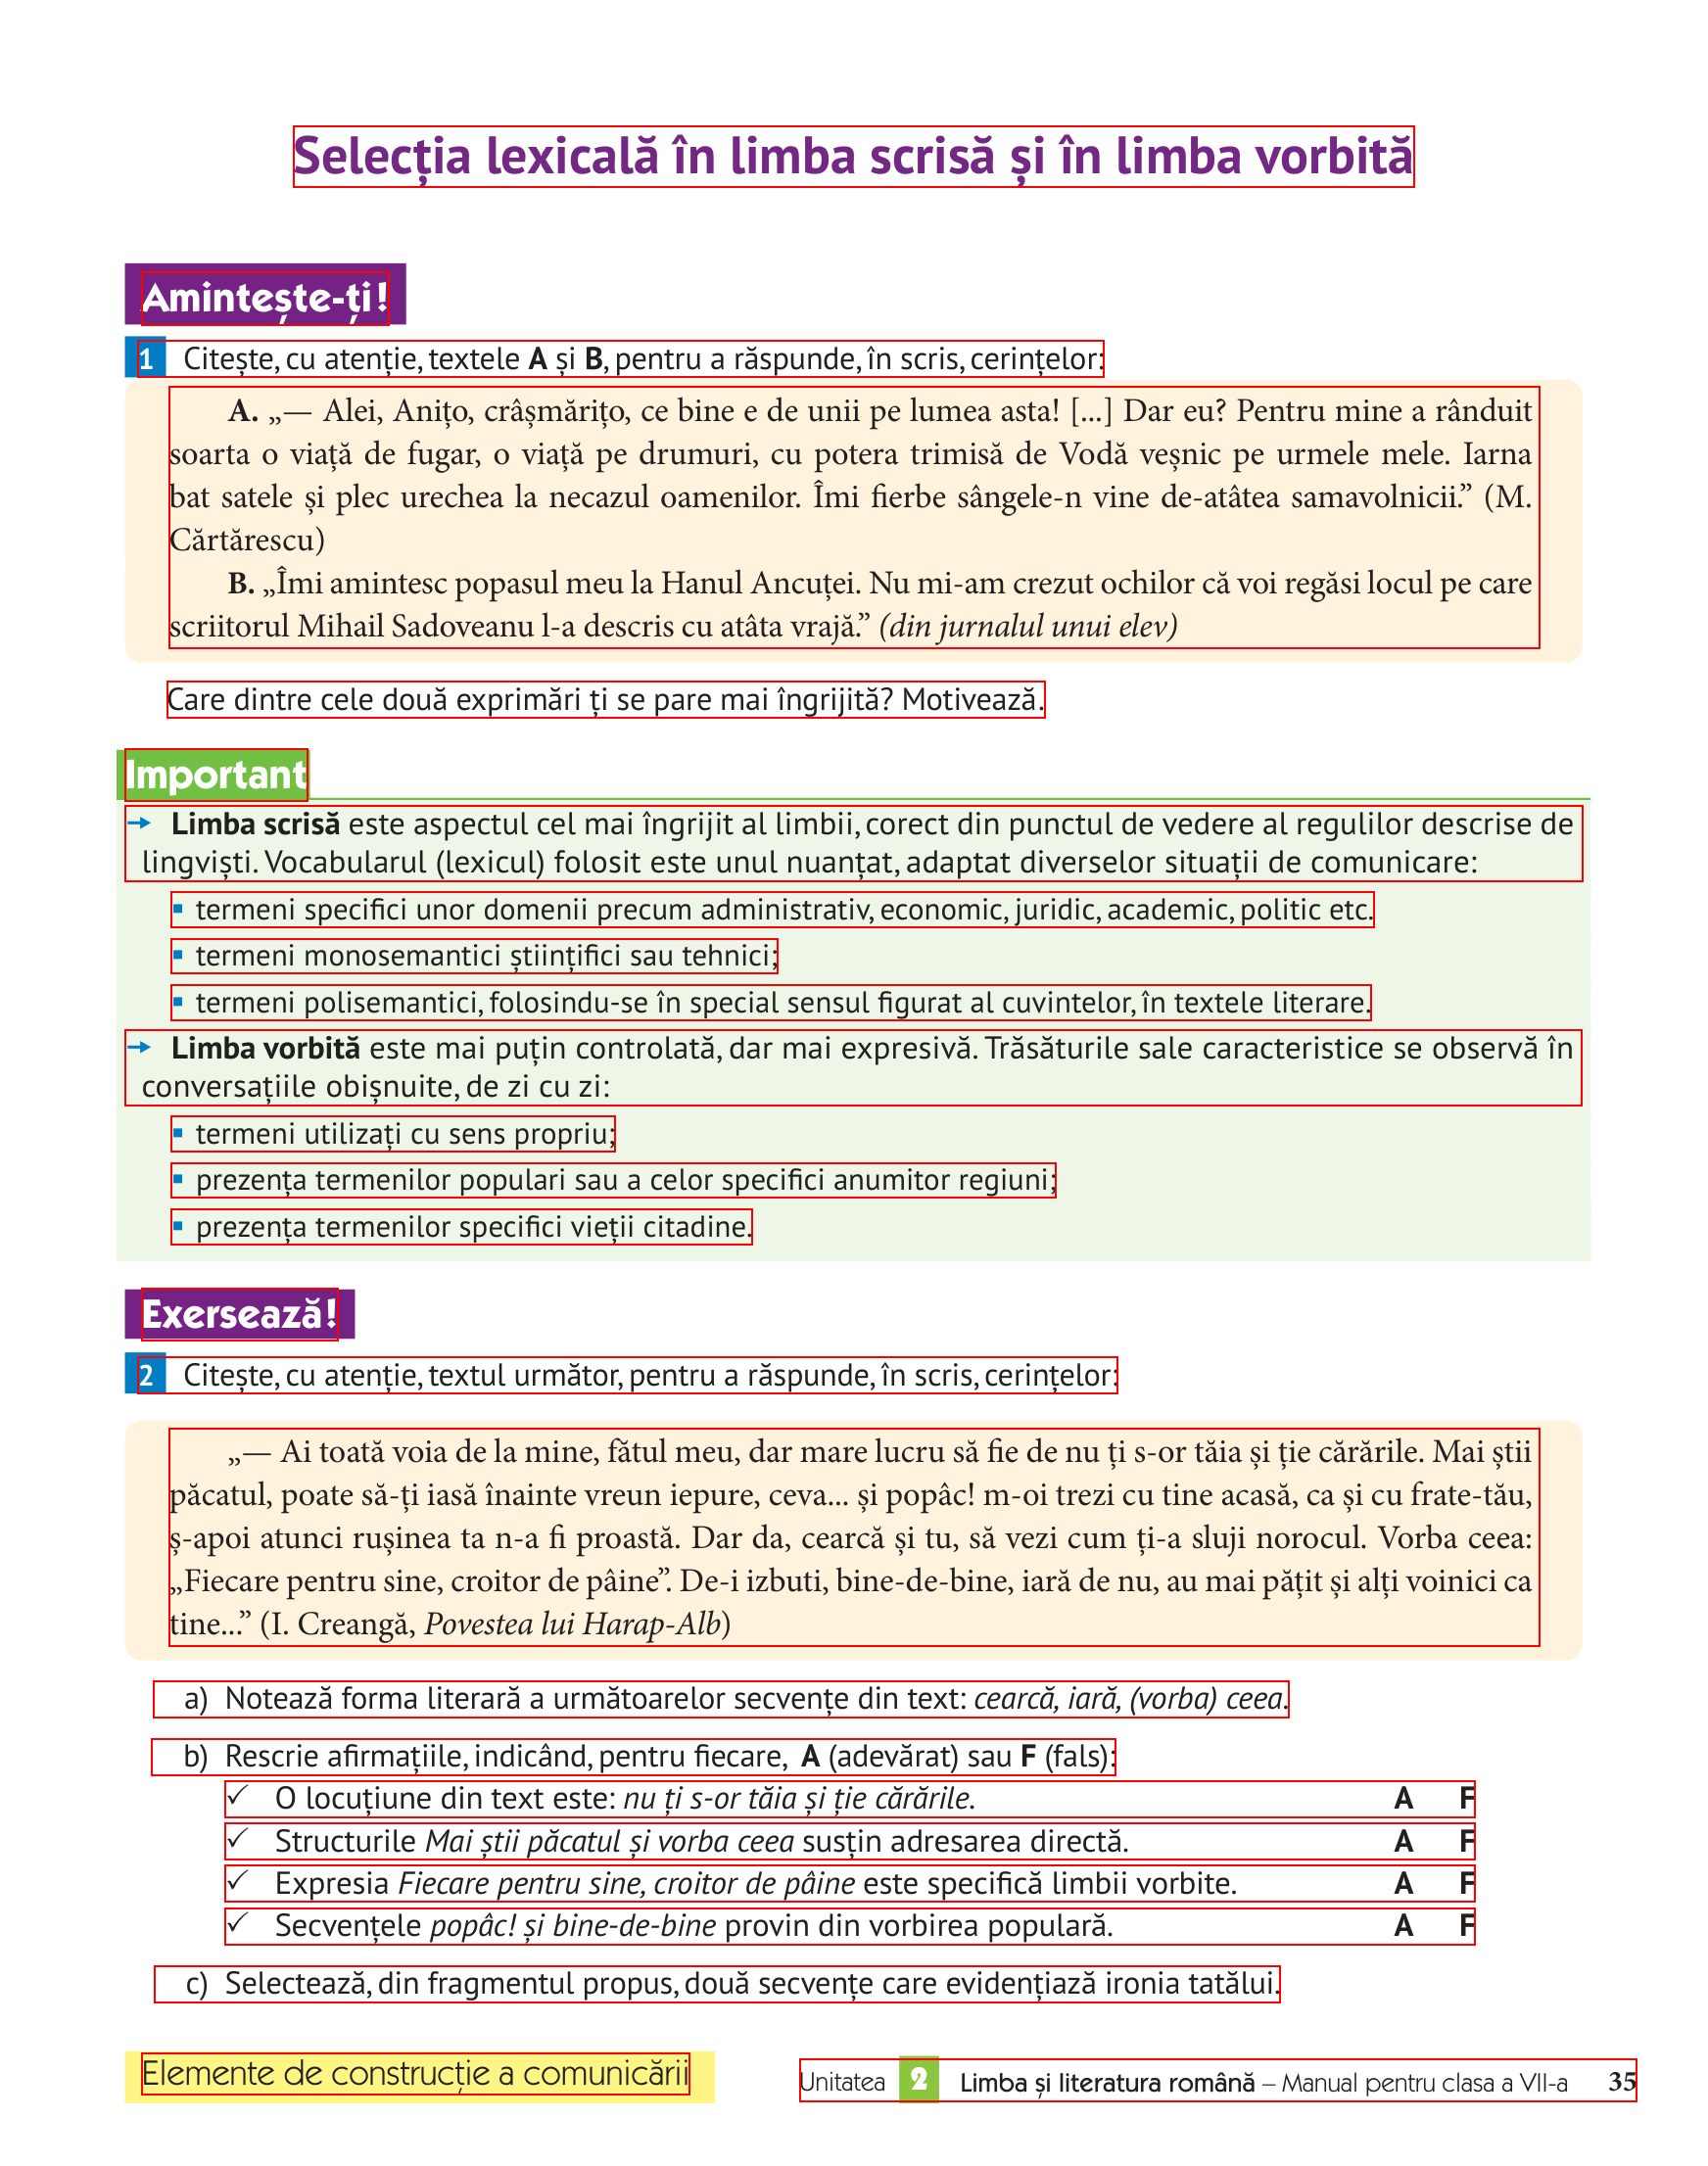
\includegraphics[scale=.2]{Figura4_5}
	\caption{Text încadrat în bbox-uri}
	\label{fig:Figura4_5}
\end{figure}

Pentru $a = d = 3$, fiecare imagine o să aibă dimensiunea de 2212x1744 px. Timpul mediu de rulare al programului pentru aceste dimensiuni ale imaginilor este de $0,4066$ secunde pe pagină. Pentru $a = d = 4$, fiecare imagine generată o să aibă dimensiunea de 2949x2325 px. Timpul mediu de rulare al programului pentru aceste dimensiuni ale imaginilor este de $0,5948$ secunde pe pagină.

După ce este găsită cea mai bună configurație pentru pagină, pixmap-ul se transformă într-o secvență de bytes, unde fiecare byte reprezintă toate informațiile necesare pentru a recrea o imagine. Câteva caracteristici sunt: identificarea tipului de imagine (PNG, JPG etc.), dimensiunea, culorile fiecărui pixel.

După acest pas, se extrage cea mai frecventă culoare din bbox. Pentru a face acest lucru, se analizează culoarea fiecărui pixel, iar cea mai des întâlnită culoare este returnată în format RGB.
\vspace{3em}
\begin{lstlisting} [language=Python]
	def extract_pdf(path, page_nr): 
		'''
		Open PDF and extract text as a dictionary
		'''
		
		# Turn page into a pixmap
		zoom_factor = 3
		matrix = pymupdf.Matrix(zoom_factor, zoom_factor)
		pixmap = page.get_pixmap(matrix=matrix)
		
		# Turn pixmap into an image
		image = Image.open(io.BytesIO(pixmap.tobytes()))
		img_border = pymupdf.Rect(0, 0, image.width, image.height)
		
		for block in text_attributes_dict['blocks']:
			if block['type'] == 0:  # if type is 0 then it is a text block
			bbox = block['bbox']
				x0, y0, x1, y1 = bbox
				x0_zoomed = x0 * zoom_factor
				y0_zoomed = y0 * zoom_factor
				x1_zoomed = x1 * zoom_factor
				y1_zoomed = y1 * zoom_factor
				rect = pymupdf.Rect(x0_zoomed, y0_zoomed, x1_zoomed, y1_zoomed)
				
				if img_border.contains(rect):  # Check if text block is in image
					color = pixmap.color_topusage(clip=rect)[1]  # Most used color
					block['bg_color'] = tuple(color)
		
		'''
		Append color to attributes list
		'''
		image.close()
		pdf.close()
		return text_attributes_list
\end{lstlisting}


\subsection{Extragerea imaginilor}

Extragerea imaginilor este un pas esențial în convertirea PDF-ului în HTML. În versiunea digitală este necesară apariția tuturor imaginilor prezente deja în cea de tipar. În cazul în care unele poze nu sunt citite, ele vor fi introduse manual ulterior.

Pentru a realiza această extragere, sunt parcurși următorii pași:
\begin{itemize}
	\item găsirea tuturor imaginilor din paginile PDF;
	\item verificarea formatului imaginii;
	\item verificarea imaginii dacă este inversată;
	\item salvarea imaginii într-un fișier.
\end{itemize}

Imaginile sunt returnate sub forma unei liste de elemente unde fiecare variabilă reprezintă o caracteristică a imaginii. Cu ajutorul referinței fiecărei imagini, aceasta se poate transforma într-un pixmap. Informațiile despre imagini sunt:
\begin{center}
	[xref, smask, width, height, bpc, colorspace, alt. colorspace, name, filter]
\end{center}

\begin{itemize}
	\item \textbf{xref}: referința de la imagine.
	\item \textbf{smask}: referința de la masca imaginii (masca imaginii este un nivel de transparență care se pune peste imagine).
	\item \textbf{width}: lățimea imaginii.
	\item \textbf{height}: înălțimea imaginii.
	\item \textbf{bpc}: numărul de biți (de obicei 8).
	\item \textbf{colorspace}: numele spațiului de culoare (RGB, CMYK, etc.).
	\item \textbf{alt. colorspace}: numele unui alt spațiu de culoarea (dacă este cazul).
	\item \textbf{name}: numele imaginii.
	\item \textbf{filter}: numele filtrului de decodare a imaginii (se referă la cum a fost comprimată imaginea în PDF).
\end{itemize}

CMYK este un spațiu de culoare și face referire la următoarele culori: cyan, magenta, yellow și key (black). Spațiul este predominant folosit pentru documentele care urmează a fi tipărite. La fel ca și CMYK, un alt spațiu de culoarea este RGB. Acronimul vine de la red, green, blue și este folosit pentru afișarea obiectelor pe orice tip de display.

O altă diferență între cele două spații de culoare este modul în care sunt folosite. Pentru a folosi formatul RGB se va alege un număr între 0 și 255 pentru fiecare culoarea. Fiecărui canal (R, G, B) i se atribuie 8 biți. Pentru formatul CMYK va fi ales un procent de la 0\% la 100\%.  
\begin{center}
	Albastru în format RGB:
	(0, 0, 255)
	
	Albastru în format CMYK:
	(100\%, 100\%, 0\%, 0\%)
\end{center}

La crearea manualului tipărit în Adobe InDesign, imaginile sunt ilustrate în format CMYK. Pentru a crea varianta digitală a unui manual, este necesar ca imaginile să fie transformate în format RGB, acesta fiind un spațiu nativ pentru display-uri \cite{anderson1996proposal}.

Pentru verificarea tipului de imagine este necesară verificarea numărului de componente ale unui pixel și nivelul de transparență. Dacă diferența dintre numărul de componente și nivelul de transparență este mai mare de 3, atunci imaginea este în format CMYK și trebuie să fie convertită în format RGB.

O variantă mai simplă ar fi fost să fie verificat atributul spațiului de culoare (colorspace). Această metodă nu ar fi funcționat deoarece pixmap-urile suportă doar trei spații de culoare: gray, RGB, CMYK. În general, există mai multe formatări de culoare. O metodă consistentă pentru verificare este cea descrisă mai sus în care este verificat numărul de componente al unui pixel.

În cazul unor imagini, există posibilitatea să fie inversate. Acest lucru se datorează modului în care au fost salvate pozele când au fost introduse în manual. Mai exact, a fost aplicată o matrice de transformare asupra lor. 

Pentru a verifica dacă imaginea este salvată în mod corect, se identifică matricea de transformare și, mai exact, primul parametru al acesteia. Dacă parametrul este negativ înseamnă că poza este inversată.

\vspace{3em}

Funcția care extrage imaginile este:
\vspace{1em}
\begin{lstlisting} [language=Python]
	def extract_pdf(path, page_nr):
		'''
		Open PDF and extract text as a dictionary
		'''
		
		'''
		Turn page into a pixmap
		'''
	
		# Extract images and save them to images directory
		image_list = page.get_images()
		for image_index, img in enumerate(image_list, start=1):
			xref = img[0]
			pix = pymupdf.Pixmap(pdf, xref)
			transform = page.get_image_info(xrefs=True)[image_index-1]['transform']
			if pix.n - pix.alpha > 3:
				pix = pymupdf.Pixmap(pymupdf.csRGB, pix)
			if transform[0] < 0:
				pix_image = Image.open(io.BytesIO(pix.tobytes()))
				pix_image = pix_image.transpose(method=Image.FLIP_LEFT_RIGHT)
				pix_image.save("manuale/Romana_nou/images/page_%s-image_%s.png" % (page_nr, image_index))
			elif img[5] != 'DeviceCMYK':
				pix.pil_save("manuale/Romana_nou/images/page_%s-image_%s.png" % (page_nr, image_index))
			else:
				pix.save("manuale/Romana_nou/images/page_%s-image_%s.png" % (page_nr, image_index))
			pix = None
		
		'''
		Turn page into a pixmap and append everything to the list
		'''
		
		image.close()
		pdf.close()
		return text_attributes_list
\end{lstlisting}
\vspace{1em}

Imaginile recunoscute de program și salvate au următorul format:

\begin{center}
	[numele pozei, 0 , '', 0, (256, 0, 0)]
\end{center}

Au fost alese aceste valori pentru a le diferenția de alte elemente de text, iar la culoarea de fundal a fost pus 256 pentru a fi clar că este o imagine. Un segment de text ar putea avea valori numai între 0 și 255.


\section{Curățare}

Al doilea pas este curățarea textului rezultat. Principalele elemente care vor fi eliminate sunt: spațiile goale, formulele de matematică și fizică, segmentele de text din subsolul paginii.

Formulele de matematică și fizică nu sunt recunoscute de librăria cu care este extras textul. Singurul lucru care este afișat la formule este \textbf{/uf072}. Având în vedere că toate formulele au același format, ele nu pot fi recunoscute, deci vor fi eliminate din baza de date.

Recunoașterea expresiilor matematice în documente digitale este o problemă care este studiată încă din anul 1967 \cite{anderson1967syntax} de Robert H. Anderson. În lucrările recente \cite{baker2010faithful}, au fost studiate metode de recunoaștere a formulelor prin OCR (Optical Character Recognition). Paginile PDF se transformă în imagini, iar expresiile sunt recunoscute după forma lor.

O alternativă care dă rezultate foarte bune este un algoritm  bazat pe mărimea obiectelor din PDF. Lucrarea \cite{wang2019extraction} de cercetare despre acest subiect a fost publicată în 2019 și prezintă un algoritm care are o precizie de 93,6 \%.

Pe lângă aceste formule, unele porțiuni de text vor fi scoase deoarece urmează să fie înlocuite cu imagini.

Pentru a realiza curățarea, se iterează prin lista de elemente și se verifică anumite criterii:
\begin{itemize}
	\item \textbf{Spații}:
	\begin{lstlisting} [language=Python]
		elif text == ' ':
		# Remove empty spaces
		i += 1\end{lstlisting}
	
	\item \textbf{Formule}:
	\begin{lstlisting} [language=Python]
		elif text == "\uf072":
		# Remove math/physics formulas
		i += 1\end{lstlisting}
	\item \textbf{Text înlocuit cu imagini}:
	\begin{lstlisting} [language=Python]
		elif bkgr_color == (255, 241, 214):
		# remove 'Citeste si' text box with specific background color (light beige)
		i += 1\end{lstlisting}
	\begin{figure}[H]
		\centering
		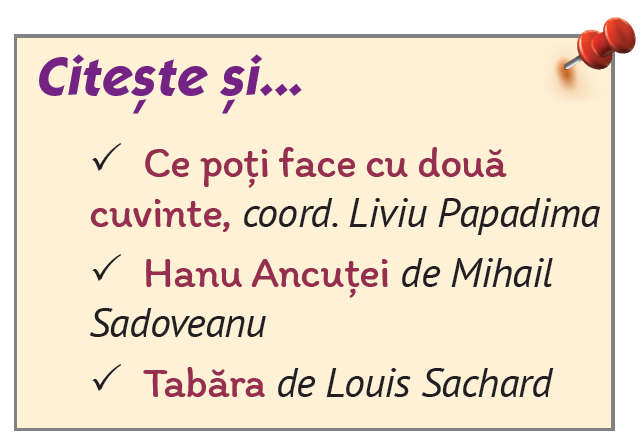
\includegraphics[scale=.3]{Figura4_6}
		\caption{Exemplu de text care va fi eliminat și înlocuit cu o imagine}
		\label{fig:Figura4_6}
	\end{figure}
	\vspace{8em}
	\item \textbf{Text din subsolul paginii}:
	\begin{lstlisting} [language=Python]
		elif size == 9.0 and font == 'ITCKabelStd-MediumRO' and text_attributes_list[i + 1][0] == ' – Manual pentru clasa a VII-a':
		# remove text besides page number
		i += 5\end{lstlisting}
	\begin{figure}[H]
		\centering
		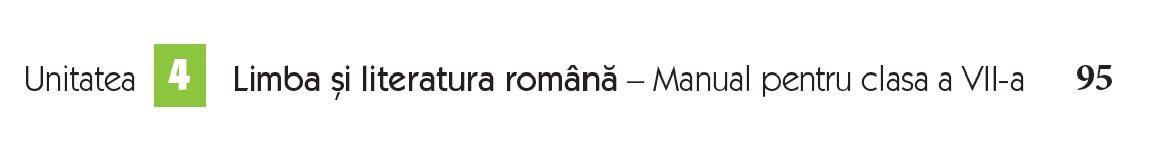
\includegraphics[scale=.8]{Figura4_7}
		\caption{Exemplu de text din subsolul paginii}
		\label{fig:Figura4_7}
	\end{figure}
\end{itemize}

Mai jos este o comparație între setul de date înainte și după ce a fost curățat.
\begin{table}[H]
	\centering
	\begin{minipage}{0.45\textwidth}
		\centering
		\begin{tabular}{|c|c|}
			\hline
			 & Text \\
			\hline
			1 & – Manual pentru clasa a VII-a \\
			\hline
			2 & Unitatea \\
			\hline
			3 & 19 \\
			\hline
			4 & 2 \\
			\hline
			5 & 4 \\
			\hline
			6 & Scrie câte un sinonim potrivit în \\
			\hline
			7 & text pentru fiecare dintre cuvintele: \\
			\hline
			8 &  \\
			\hline
			9 & 3 \\
			\hline
			10 & se înființă; \\
			\hline
			11 &  \\
			\hline
			12 & 3 \\
			\hline
			13 & să se-ntremeze; \\
			\hline
			14 &  \\
			\hline
			15 & 3 \\
			\hline
			16 & bat (satele); \\
			\hline
			17 &  \\
			\hline
			18 & 3 \\
			\hline
			19 & mă încolțește; \\
			\hline
		\end{tabular}
		\caption{Set de date înainte să fie curățat}
	\end{minipage}
	\hfill
	\begin{minipage}{0.45\textwidth}
		\centering
		\begin{tabular}{|c|c|}
			\hline
			& Text \\
			\hline
			1 & 4 \\
			\hline
			2 & Scrie câte un sinonim potrivit în \\
			\hline
			3 & text pentru fiecare dintre cuvintele: \\
			\hline
			4 & 3 \\
			\hline
			5 & se înființă; \\
			\hline
			6 & 3 \\
			\hline
			7 & să se-ntremeze; \\
			\hline
			8 & 3 \\
			\hline
			9 & bat (satele); \\
			\hline
			10 & 3 \\
			\hline
			11 & mă încolțește; \\
			\hline
		\end{tabular}
		\caption{Set de date după ce a fost curățat}
	\end{minipage}
\end{table}


\section{Grupare}

După ce a fost extras și curățat textul, acesta trebuie grupat. Gruparea se face pe mai multe niveluri. Primul nivel începe din interiorul textului de la cuvinte și ajunge până la fragmente întregi de text.

Două dintre cele mai des întâlnite motive pentru care segmentele de text se despart sunt: atunci când textul nu are același font peste tot, atunci când textul este scris pe un rând și se continuă pe altul.

\vspace{1em}
Pentru prima problemă va fi ilustrat un exemplu din manual în figura 4.8.
\begin{figure}[H]
	\centering
	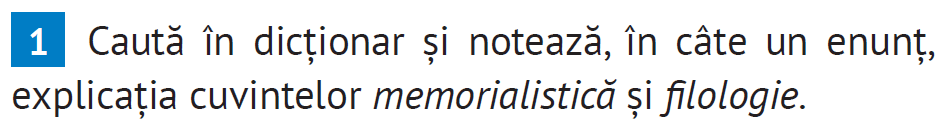
\includegraphics[scale=.35]{Figura5_1}
	\caption{Text preluat din manual}
	\label{fig:Figura5_1}
\end{figure}

Acest text se separă în felul următor:
\begin{table}[H]
	\centering
	\begin{tabular}{|l|l|l|}
		\hline
		Text                                               & Size & Font              \\ \hline
		"Caută în dicționar și notează, în câte un enunț," & 11   & "PT-Sans-Regular" \\ \hline
		"explicația cuvintelor"                            & 11   & "PT-Sans-Regular" \\ \hline
		"memorialistică"                                   & 11   & "PT-Sans-Italic"  \\ \hline
		"și"                                               & 11   & "PT-Sans-Regular" \\ \hline
		"filologie"                                        & 11   & "PT-Sans-Italic"  \\ \hline
	\end{tabular}
	\caption{Exemplu de text separat din cauza fontului și din cauza trecerii pe un rând nou}
\end{table}

Obiectivul de la acest pas este de a avea același font peste tot. Pentru a realiza acest lucru se vor transforma textele cu fonturi diferite (în cazul de față italic) într-un text cu font simplu, adăugându-i formatul HTML. Pentru a identifica ce texte se pot formata, se identifică numele fontului.
\begin{figure}[H]
	\centering
	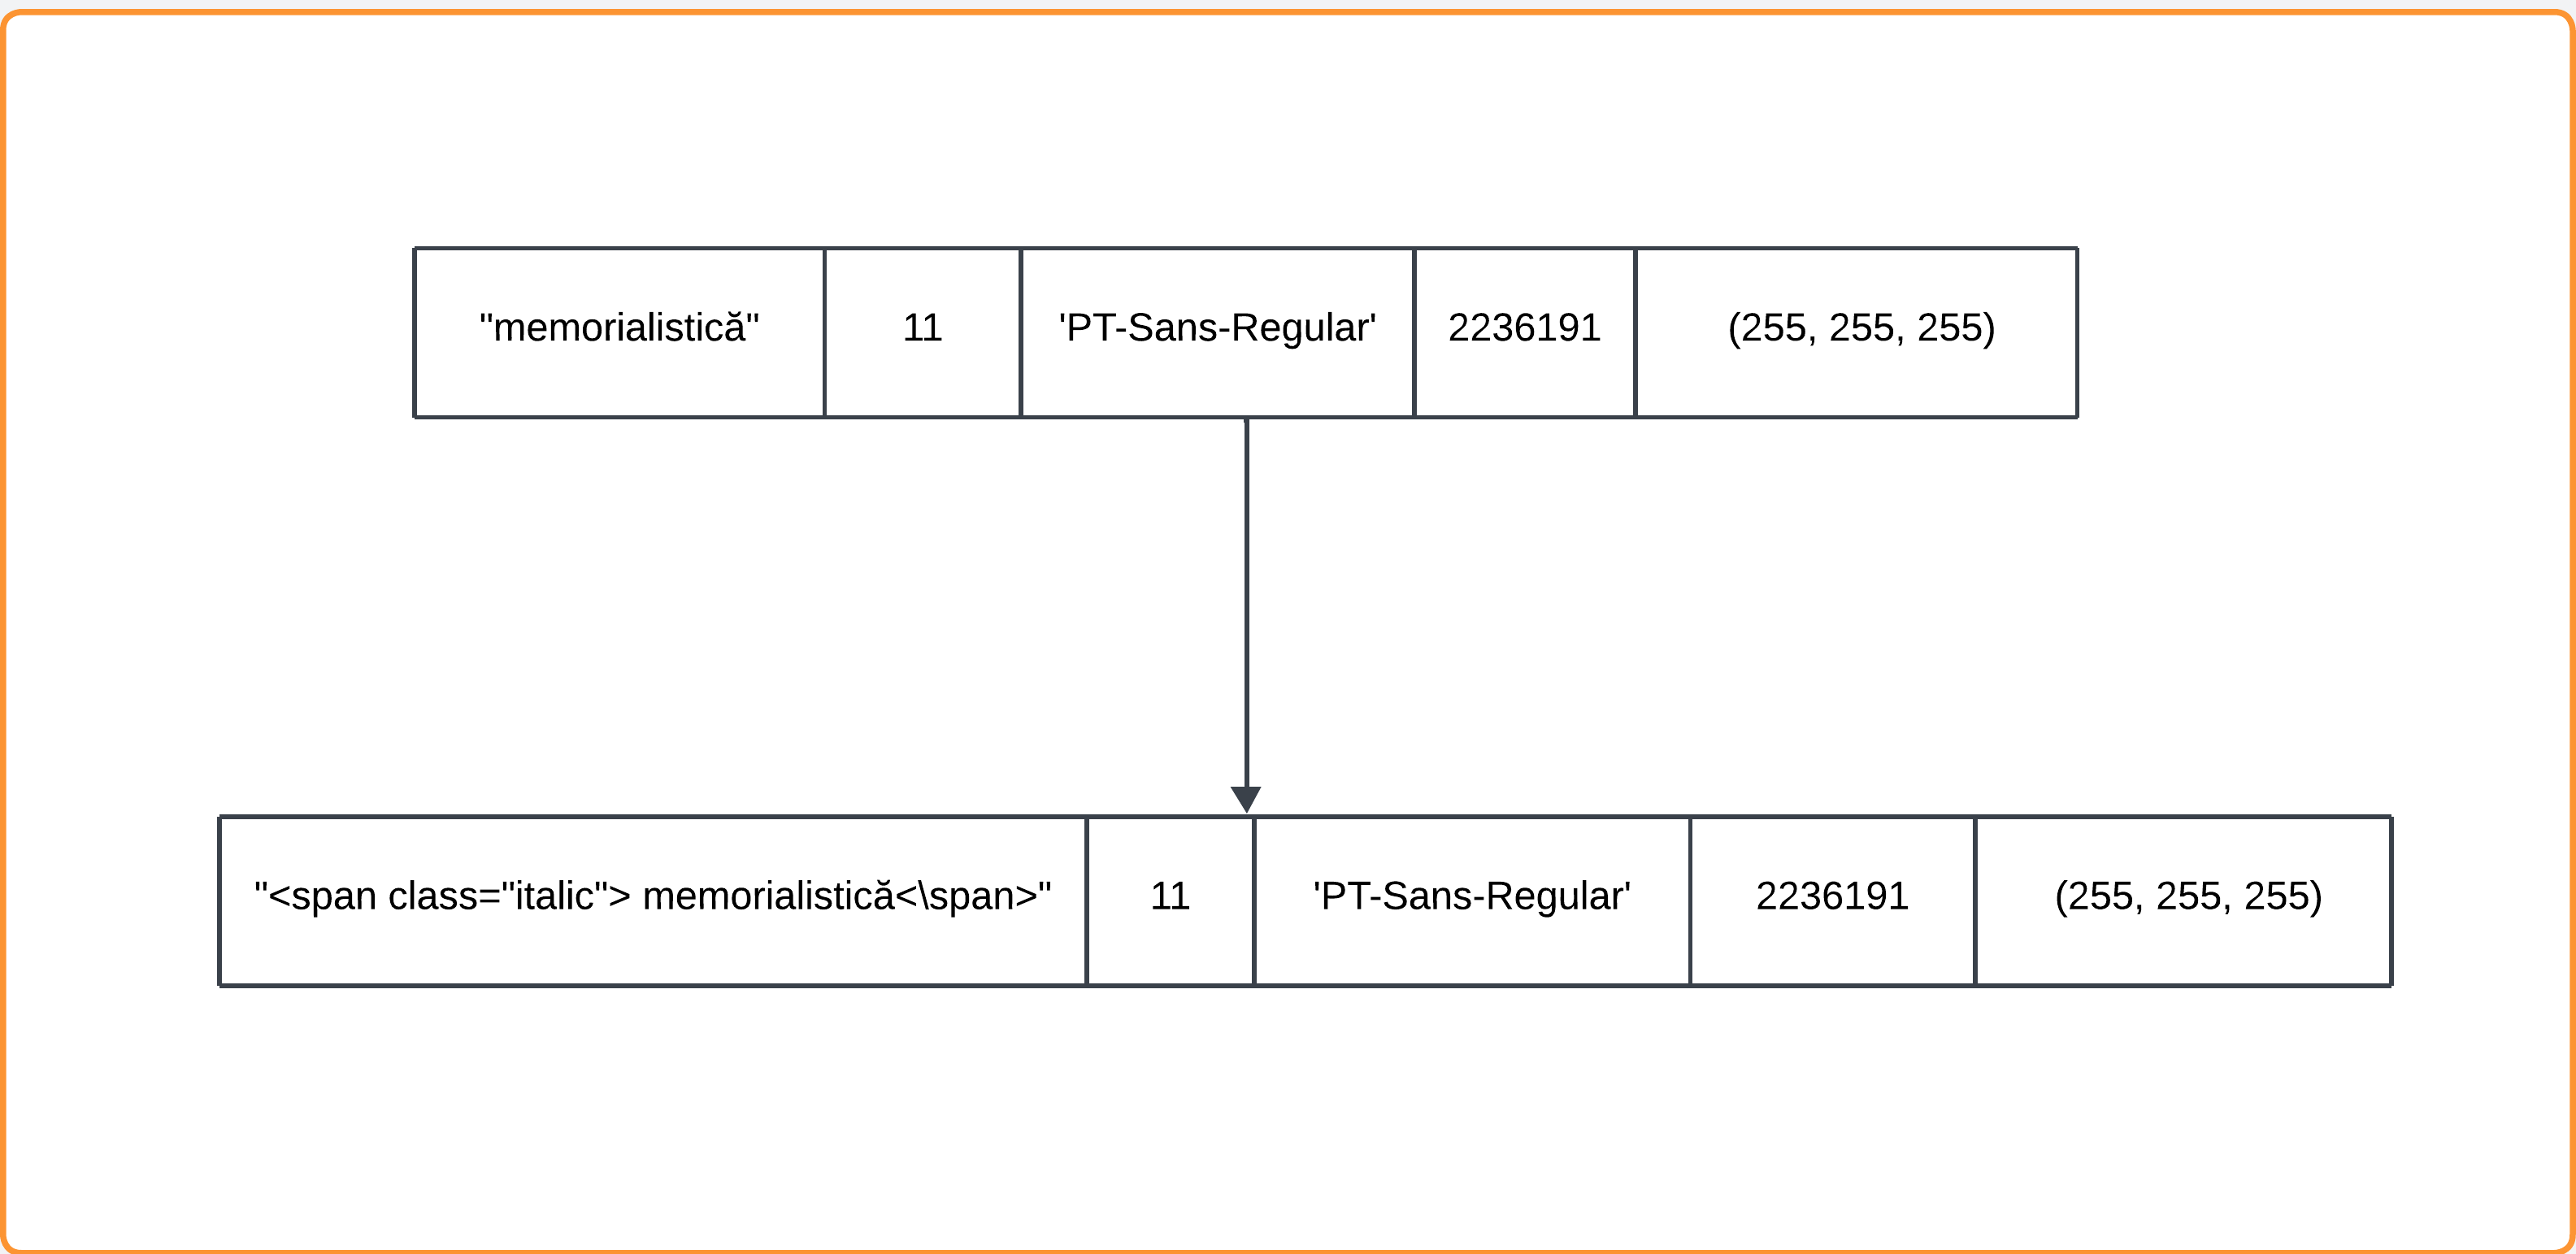
\includegraphics[scale=.45]{Figura5_2}
	\caption{Formatare a textului în HTML}
	\label{fig:Figura5_2}
\end{figure}

După ce este realizată schimbarea de font, se trece la următoarea problemă. Mai precis, cum se grupează textul scris pe mai multe rânduri.

Este construită o funcție în care se verifică pe rând dacă 2 elemente au aproximativ aceeași mărime (marjă de 0.2 points), același font și aceeași culoarea de fundal și după le combinăm.
\vspace{1em}
\begin{lstlisting} [language=Python]
	def combine_text(text_attributes_list):
		# Combine text with the same size, font and background color
		new_text_attributes_list = []
		previous_text = ""
		previous_size = 0
		previous_font = ""
		previous_color = 0
		previous_bg_color = (0, 0, 0)
		for element in text_attributes_list:
			text, size, font, color, bg_color = element
			if previous_size - 0.2 <= size <= previous_size + 0.2 and font == previous_font and bg_color == previous_bg_color:
				previous_text += " " + text
			else:
				if previous_text:
					new_text_attributes_list.append([previous_text, previous_size, previous_font, previous_color, previous_bg_color])
				previous_text = text
				previous_size = size
				previous_font = font
				previous_color = color
				previous_bg_color = bg_color
		
		if previous_text:
			new_text_attributes_list.append([previous_text, previous_size, previous_font, previous_color, previous_bg_color])
		
		return new_text_attributes_list
\end{lstlisting}
\vspace{1em}


După ce este realizată gruparea la primul nivel, se va aborda gruparea fragmentelor mai lungi.


\subsection{Exerciții}

Fragmentul de exerciții este cel mai des întâlnit paragraf dintr-un manual școlar. În figura 4.10 este ilustrat un astfel de exemplu.
\begin{figure}[H]
	\centering
	
\includegraphics[scale=.4]{Figura5_3}
	\caption{Exemplu de exercițiu}
	\label{fig:Figura5_3}
\end{figure}

Textul este extras conform pașilor anteriori.
\begin{table}[H]
	\centering
	\begin{tabular}{|p{5cm}|l|l|l|l|}
		\hline
		Text                                                                   & Size   & Font              & Text color & Background color \\ \hline
		"3"                                                                    & 9.8995 & "PT-Sans-Bold"    & 16777215   & (255, 255, 255)  \\ \hline
		"Alcătuiește familia lexicală a cuvintelor țară, pădure, bun, a face." & 10.78  & "PT-Sans-Regular" & 2236191    & (255, 255, 255)  \\ \hline
	\end{tabular}
	\caption{Segment de text după pașii de curățare și grupare}
\end{table}

Dacă pașii de grupare de dinainte au avut succes, în baza de date o să rămână numărul exercițiului și cerința. Doar numerele de la exerciții au mărimea de 9.8995 points și culoarea de 16777215. Așadar, se vor identifica numerele de la exerciții după aceste 2 criterii, va fi selectat textul următor, și vor fi introduse într-un block de exercițiu.
\vspace{1em}
\begin{lstlisting} [language=html]
	<div class="block-container">
		<span class="number">{text}</span>
		<div class="block-number-content">
			<p>{text2}</p>
		</div>
	</div>
	<p class="clear"></p>\n
\end{lstlisting}
\vspace{1em}

Variabilele text attributes list[i] și [i+1] reprezintă numărul exercițiului, respectiv textul care urmează după el. După ce am sunt transformate cele 2 elemente separate într-un singur block de HTML, ele sunt intorduse înapoi în baza de date.


\subsection{Liste ordonate}

De multe ori cerințele de la enunțuri conțin și subpuncte. Acestea sunt tratate sub forma unor liste ordonate din HTML (ordered list).
\begin{figure}[H]
	\centering
	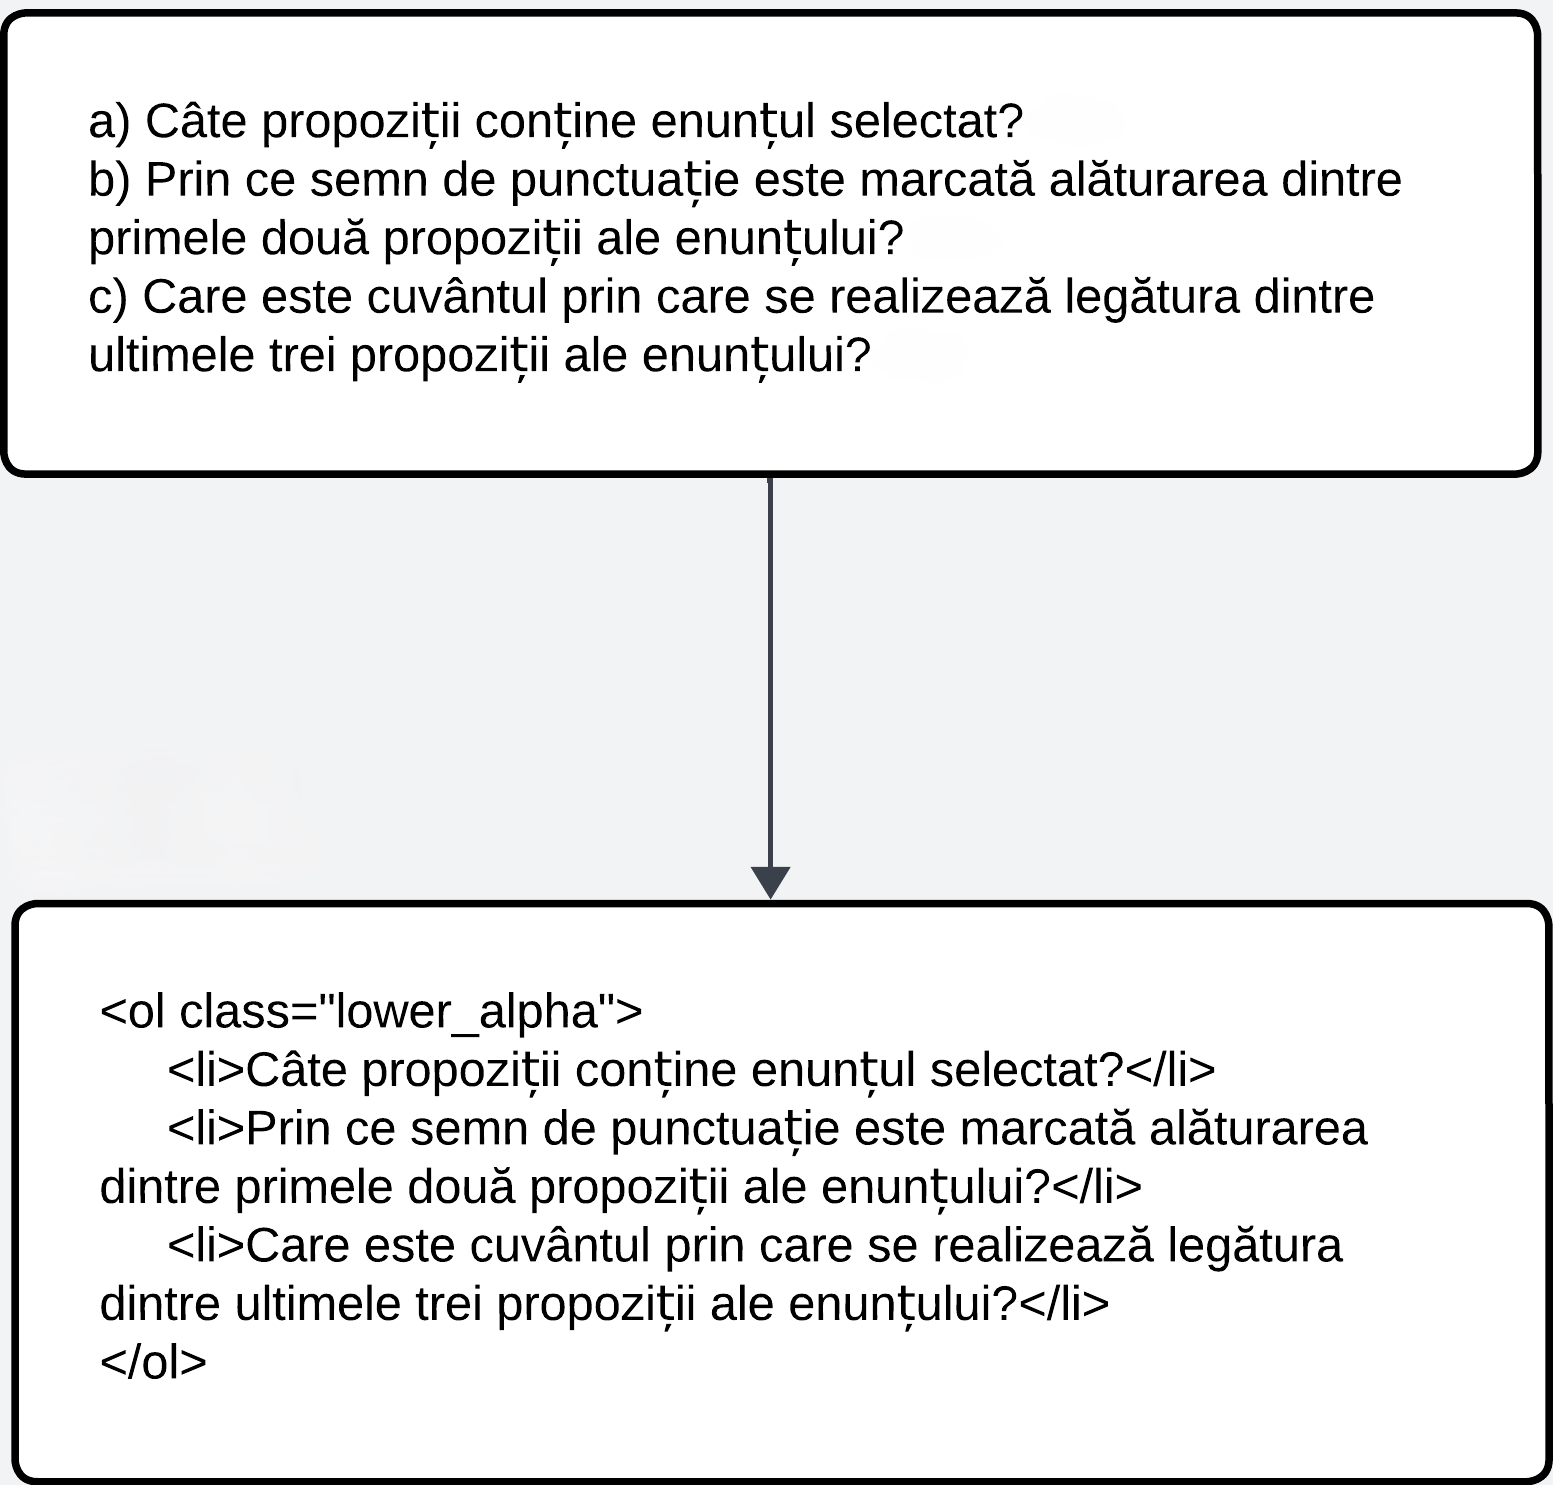
\includegraphics[scale=.5]{Figura5_4}
	\caption{Exemplu de liste transformate în HTML}
	\label{fig:Figura5_4}
\end{figure}

Atunci când este extras textul, aceste subpuncte sunt identificate ca o singură porțiune de text. Așadar, se desparte textul în funcție de numele subpunctului. 
\begin{center}
	pattern = r'\textbackslash s(?=[a-z]\textbackslash))
	
	result = re.split(pattern, text)
\end{center}

După aceea, se iterează prin lista de elemente cu subpuncte și se adaugă în formatul HTML.
\vspace{1em}
\begin{lstlisting} [language=Python]
	list_items_html = f'''
			<ol class="lower_alpha">
	'''
	for k in range(1, len(result)):
		list_items_html += f'''
				<li>{result[k][2:]}</li>
	'''
	list_items_html += f'''
			</ol>
	'''
\end{lstlisting}
\vspace{1em}

În baza de date, subpunctele sunt văzute ca o singură porțiune de text, iar ele vor fi separate și după reintorduse.


\subsection{Liste neordonate}

Listele neordonate care apar în manuale sunt de 3 feluri, în funcție de caracterul folosit pentru listare (bullet point etc.). Pentru fiecare caz va fi aplicat același algoritm.

Algoritmul propus este următorul: se creează 2 liste auxiliare; o listă mare în care vor fi toate elementele și o listă mică în care sunt doar elementele cu caracter special. În final, se va itera prin lista mare și va fi verificat dacă elementele au o structură de liste. După aceea, se va adăuga segmentul de text HTML care deschide și închide o listă neordonată (unordered list).


\subsection{Paragrafele "Important"}

Acest tip de paragrafe sunt motivul principal pentru care a trebuit să se extragă și culoarea de fundal a fiecărui segment de text. Aceste paragrafe au același format în care se începe cu numele "Important" care are un fundal verde închis, iar textul din cadrul acestui paragraf apare cu un verde mai deschis.
\begin{figure}[H]
	\centering
	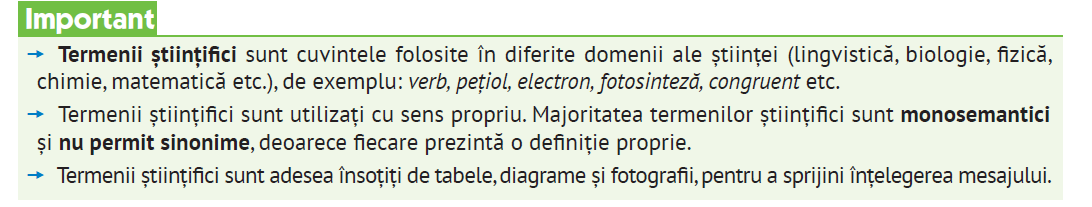
\includegraphics[scale=0.5]{Figura5_5}
	\caption{Exemplu de paragraf "Important"}
	\label{fig:Figura5_5}
\end{figure}

Problema de dinainte cu aceste tipuri de fragemente era faptul că nu se putea determina până unde se continuă un text cu fundal verde. Astfel, a fost nevoie de un nou atribut, și anume culoarea de fundal. Folosind această caracteristică, se poate verifica până unde se extinde textul dintr-un paragraf de tipul "Important".

Soluția găsită pentru acest tip de fragmente este următoarea: se grupează textul la fel ca la pașii anteriori, dacă există elemente care nu au fost grupate atunci ele vor fi adăugate conform culorii de fundal, se adaugă tot conținutul într-un div.

\vspace{1em}
\begin{lstlisting} [language=html]
	<h3 class="important">Important</h3>
	<div class="bkgr-imp">
		{text_imp}
	</div>
\end{lstlisting}

\section{Scriere}

După ce au fost parcurși toți pașii de curățare și grupare, mai rămâne doar partea de scriere. 

Se iterează prin lista de elemente și se verifică dacă acestea pot fi introduse în  fișierul HTML sau nu. Astfel, vor exista 3 tipuri de elemente în baza de date, conform tabelului de mai jos.
\begin{table}[H]
	\centering
	\begin{tabular}{|l|l|l|l|l|}
		\hline
		Text             & Size & Font        & Text color & Background color \\ \hline
		"some text"      & 0    & "0"         & 0          & (257, 0, 0)      \\ \hline
		"some image"     & 0    & "0"         & 0          & (256, 0, 0)      \\ \hline
		"other elements" & 123  & "some font" & 123        & (123, 123, 123)  \\ \hline
	\end{tabular}
	\caption{Tipuri de date rămase}
\end{table}

A fost realizată următoarea notație:

\begin{itemize}
	\item \textbf{Textul pregătit de scriere}: toate atributele vor fi notate cu 0, în afara de cel de la culoarea de fundal, care va fi notat cu 257. 
	\item \textbf{Imaginea}: toate atributele vor fi notate cu 0, în afara de cel de la culoarea de fundal, care va fi notat cu 256. 
	\item \textbf{Textul care nu este pregătit de scriere}: atributele nu se vor schimba. 
\end{itemize}

Au fost alese aceste caracteristici deoarece valorile culorii de fundal pot fi numai de la 0 la 255. Astfel, este mai ușor de identificat ce elemente sunt gata de introdus în fișierul HTML și ce elemente vor fi adăugate manual.
\chapter{Concluzie}

\section{Rezultate}

Pentru a verifica eficiența soluției propuse, se măsoară trei aspecte: viteza de procesare, procentul de similaritate dintre manualul tipărit și manualul digital în forma inițială (așa cum este obținut din aplicația de automatizare), procentul de similaritate dintre varianta digitală inițială și varianta digitală finală (după ce a fost prelucrat astfel încât să corespundă în totalitate cu manualul tipărit).

Testarea este efectuată pe un manual de 203 pagini. Aplicația de automatizare obține un timp de 354.8057 secunde sau 5.9314 minute, ceea ce înseamnă 1.747 de secunde pe pagină.

Pentru a compara varianta tipărită cu varianta digitală inițială, se vor realiza etapele următoare: convertirea ambelor variante de manuale în text simplu, despărțirea textului în cuvinte, verficiarea numărului de șiruri de cuvinte care apar în ambele variante. 

Pentru a realiza această comparație se va folosi următoarea formulă:

\begin{center}
	\[
	\text{ratio} = 2.0 \cdot \frac{M}{T}
	\]
\end{center}


\begin{itemize}
	\item \( M \) este numărul de șiruri de cuvinte consecutive care apar în ambele manuale.
	\item \( T \) este numărul total de cuvinte din cele două manuale.
\end{itemize}

Astfel, procentul de similaritate dintre variantă tipărită și varianta digitală produsă de aplicație este de 69,13\%. Din variantă tipărită a fost extras și textul care face parte din imagini, numărul paginilor, tabele. Aceste porțiuni de text nu au fost extrase și în varianta digitală deoarece ele vor fi înlocuite cu poze sau vor fi eliminate. Procentul practic de similaritate o să fie puțin mai ridicat.

Procentul de similaritate dintre varianta inițială și varianta finală este de 72,35\%, iar procentul de similaritate dintre varianta finală a manualului digital și varianta tipărită este de 85,58\%. 


\begin{table}[H]
	\centering
	\begin{tblr}{
			cell{1}{1} = {c=3}{},
			hlines,
			vlines,
		}
		Procent de similaritate între manuale &            &            \\
		$\mathrm{MD}_1$ vs $\mathrm{MT}$     & $\mathrm{MD}_1$ vs $\mathrm{MD}_2$ & $\mathrm{MD}_2$ vs $\mathrm{MT}$~ \\
		69,13\%                               & 72,35\%    & 85,58\%    
	\end{tblr}
	\caption{Procent de similaritate între manualul tipărit, manualul digital inițial și manualul digital final}
\end{table}


\begin{itemize}
	\item $\mathrm{MD}_1$ este manualul digital inițial, așa cum este generat de aplicația de automatizare.
	\item $\mathrm{MD}_2$ este manualul digital în forma finală, după ce au fost realizate toate modificările necesare.
	\item $\mathrm{MT}$ este manualul tipărit, în format PDF.
\end{itemize}

Scopul aplicației este de a automatiza un proces de conversie și de a economisi cât mai mult timp. Procentul de similaritate dintre manualul digital inițial și varianta finală a acestuia este de 72,35\%. Durata de procesare a aplicației este de aproximativ 6 minute. Pe lângă acest timp de execuție, este luat în considerare și timpul petrecut pentru realizarea completă a manualului digital (restul de 27,65\%), însemnând aproape 6 zile.

Rezultatul final produs de aplicația de automatizare este timpul de conversie redus de la 3 săptămâni la aproximativ 6 zile.


\section{Îmbunătățiri pentru viitor}

În viitor, prioritatea principală este de a îmbunătăți procentajul de similaritate dintre versiunea inițială generată de aplicație și versiunea finală. Acest lucru poate fi realizat prin tratarea excepțiilor, cum ar fi segmente de text care nu sunt recunoscute de aplicație.

O funcționalitate care poate fi implementată este recunoașterea formulelor de matematică și fizică din manualul PDF, utilizând OCR (Optical character recognition). Acest lucru va reduce considerabil timpul de creare al unui manual digital care conține orice tip de formule.

De asemenea, paginile HTML pot fi formatate astfel încât să aibă aceeași strucutră ca în varianta tipărită. Acest lucru se poate realiza prin identificarea coordonatelor fiecărei porțiuni de text. Chiar dacă nu este o cerință prevăzută în caietul de sarcini dat de Minister, această opțiune va ajuta la consistența vizuală dintre varianta de tipar și cea digitală.



\phantomsection
\addcontentsline{toc}{chapter}{\bibname}
\printbibliography





\end{document}